\documentclass[aps,preprint,preprintnumbers,nofootinbib,showpacs,prd]{revtex4-1}
\usepackage{graphicx,color}
\usepackage{caption}
\usepackage{subcaption}
\usepackage{amsmath,amssymb}
\usepackage{multirow}
\usepackage{amsthm}%        But you can't use \usewithpatch for several packages as in this line. The search 

\usepackage{cancel}

%%% for SLE
\usepackage{dcolumn}   % needed for some tables
\usepackage{bm}        % for math
\usepackage{amssymb}   % for math
\usepackage{multirow}
%%% for SLE -End

\usepackage{ulem}
\usepackage{cancel}

\usepackage{hyperref}

\usepackage[top=1in, bottom=1.25in, left=1.1in, right=1.1in]{geometry}

\usepackage{mathtools} % for \DeclarePairedDelimiter{\ceil}{\lceil}{\rceil}

\usepackage{simplewick}

\newcommand{\msout}[1]{\text{\sout{\ensuremath{#1}}}}


%%%%%% My stuffs - Stef
\newcommand{\lsim}{\mathrel{\mathop{\kern 0pt \rlap
  {\raise.2ex\hbox{$<$}}}
  \lower.9ex\hbox{\kern-.190em $\sim$}}}
\newcommand{\gsim}{\mathrel{\mathop{\kern 0pt \rlap
  {\raise.2ex\hbox{$>$}}}
  \lower.9ex\hbox{\kern-.190em $\sim$}}}

%
% Key
%
\newcommand{\key}[1]{\medskip{\sffamily\bfseries\color{blue}#1}\par\medskip}
%\newcommand{\key}[1]{}
\newcommand{\q}[1] {\medskip{\sffamily\bfseries\color{red}#1}\par\medskip}
\newcommand{\comment}[2]{{\color{red}{{\bf #1:}  #2}}}


\newcommand{\ie}{{\it i.e.} }
\newcommand{\eg}{{\it e.g.} }

%
% Energy scales
%
\newcommand{\ev}{{\,{\rm eV}}}
\newcommand{\kev}{{\,{\rm keV}}}
\newcommand{\mev}{{\,{\rm MeV}}}
\newcommand{\gev}{{\,{\rm GeV}}}
\newcommand{\tev}{{\,{\rm TeV}}}
\newcommand{\fb}{{\,{\rm fb}}}
\newcommand{\ifb}{{\,{\rm fb}^{-1}}}

%
% SUSY notations
%
\newcommand{\neu}{\tilde{\chi}^0}
\newcommand{\neuo}{{\tilde{\chi}^0_1}}
\newcommand{\neut}{{\tilde{\chi}^0_2}}
\newcommand{\cha}{{\tilde{\chi}^\pm}}
\newcommand{\chao}{{\tilde{\chi}^\pm_1}}
\newcommand{\chaop}{{\tilde{\chi}^+_1}}
\newcommand{\chaom}{{\tilde{\chi}^-_1}}
\newcommand{\Wpm}{W^\pm}
\newcommand{\chat}{{\tilde{\chi}^\pm_2}}
\newcommand{\smu}{{\tilde{\mu}}}
\newcommand{\smur}{\tilde{\mu}_R}
\newcommand{\smul}{\tilde{\mu}_L}
\newcommand{\sel}{{\tilde{e}}}
\newcommand{\selr}{\tilde{e}_R}
\newcommand{\sell}{\tilde{e}_L}
\newcommand{\smurl}{\tilde{\mu}_{R,L}}

\newcommand{\casea}{\texttt{IA}}
\newcommand{\caseb}{\texttt{IB}}
\newcommand{\casec}{\texttt{II}}

\newcommand{\caseasix}{\texttt{IA-6}}

%
% Greek
%
\newcommand{\es}{{\epsilon}}
\newcommand{\sg}{{\sigma}}
\newcommand{\dt}{{\delta}}
\newcommand{\kp}{{\kappa}}
\newcommand{\lm}{{\lambda}}
\newcommand{\Lm}{{\Lambda}}
\newcommand{\gm}{{\gamma}}
\newcommand{\mn}{{\mu\nu}}
\newcommand{\Gm}{{\Gamma}}
\newcommand{\tho}{{\theta_1}}
\newcommand{\tht}{{\theta_2}}
\newcommand{\lmo}{{\lambda_1}}
\newcommand{\lmt}{{\lambda_2}}
%
% LaTeX equations
%
\newcommand{\beq}{\begin{equation}}
\newcommand{\eeq}{\end{equation}}
\newcommand{\bea}{\begin{eqnarray}}
\newcommand{\eea}{\end{eqnarray}}
\newcommand{\ba}{\begin{array}}
\newcommand{\ea}{\end{array}}
\newcommand{\bit}{\begin{itemize}}
\newcommand{\eit}{\end{itemize}}

\newcommand{\nbea}{\begin{eqnarray*}}
\newcommand{\neea}{\end{eqnarray*}}
\newcommand{\nbeq}{\begin{equation*}}
\newcommand{\neeq}{\end{equation*}}

\newcommand{\no}{{\nonumber}}
\newcommand{\td}[1]{{\widetilde{#1}}}
\newcommand{\sqt}{{\sqrt{2}}}
%
\newcommand{\me}{{\rlap/\!E}}
\newcommand{\met}{{\rlap/\!E_T}}
\newcommand{\rdmu}{{\partial^\mu}}
\newcommand{\gmm}{{\gamma^\mu}}
\newcommand{\gmb}{{\gamma^\beta}}
\newcommand{\gma}{{\gamma^\alpha}}
\newcommand{\gmn}{{\gamma^\nu}}
\newcommand{\gmf}{{\gamma^5}}
%
% Roman expressions
%
\newcommand{\br}{{\rm Br}}
\newcommand{\sign}{{\rm sign}}
\newcommand{\Lg}{{\mathcal{L}}}
\newcommand{\M}{{\mathcal{M}}}
\newcommand{\tr}{{\rm Tr}}

\newcommand{\msq}{{\overline{|\mathcal{M}|^2}}}

%
% kinematic variables
%
%\newcommand{\mc}{m^{\rm cusp}}
%\newcommand{\mmax}{m^{\rm max}}
%\newcommand{\mmin}{m^{\rm min}}
%\newcommand{\mll}{m_{\ell\ell}}
%\newcommand{\mllc}{m^{\rm cusp}_{\ell\ell}}
%\newcommand{\mllmax}{m^{\rm max}_{\ell\ell}}
%\newcommand{\mllmin}{m^{\rm min}_{\ell\ell}}
%\newcommand{\elmax} {E_\ell^{\rm max}}
%\newcommand{\elmin} {E_\ell^{\rm min}}
\newcommand{\mxx}{m_{\chi\chi}}
\newcommand{\mrec}{m_{\rm rec}}
\newcommand{\mrecmin}{m_{\rm rec}^{\rm min}}
\newcommand{\mrecc}{m_{\rm rec}^{\rm cusp}}
\newcommand{\mrecmax}{m_{\rm rec}^{\rm max}}
%\newcommand{\mpt}{\rlap/p_T}

%%%song
\newcommand{\cosmax}{|\cos\Theta|_{\rm max} }
\newcommand{\maa}{m_{aa}}
\newcommand{\maac}{m^{\rm cusp}_{aa}}
\newcommand{\maamax}{m^{\rm max}_{aa}}
\newcommand{\maamin}{m^{\rm min}_{aa}}
\newcommand{\eamax} {E_a^{\rm max}}
\newcommand{\eamin} {E_a^{\rm min}}
\newcommand{\eaamax} {E_{aa}^{\rm max}}
\newcommand{\eaacusp} {E_{aa}^{\rm cusp}}
\newcommand{\eaamin} {E_{aa}^{\rm min}}
\newcommand{\exxmax} {E_{\neuo \neuo}^{\rm max}}
\newcommand{\exxcusp} {E_{\neuo \neuo}^{\rm cusp}}
\newcommand{\exxmin} {E_{\neuo \neuo}^{\rm min}}
%\newcommand{\mxx}{m_{XX}}
%\newcommand{\mrec}{m_{\rm rec}}
\newcommand{\erec}{E_{\rm rec}}
%\newcommand{\mrecmin}{m_{\rm rec}^{\rm min}}
%\newcommand{\mrecc}{m_{\rm rec}^{\rm cusp}}
%\newcommand{\mrecmax}{m_{\rm rec}^{\rm max}}
%%%song

\newcommand{\mc}{m^{\rm cusp}}
\newcommand{\mmax}{m^{\rm max}}
\newcommand{\mmin}{m^{\rm min}}
\newcommand{\mll}{m_{\mu\mu}}
\newcommand{\mllc}{m^{\rm cusp}_{\mu\mu}}
\newcommand{\mllmax}{m^{\rm max}_{\mu\mu}}
\newcommand{\mllmin}{m^{\rm min}_{\mu\mu}}
\newcommand{\mllcusp}{m^{\rm cusp}_{\mu\mu}}
\newcommand{\elmax} {E_\mu^{\rm max}}
\newcommand{\elmin} {E_\mu^{\rm min}}
\newcommand{\elmaxw} {E_W^{\rm max}}
\newcommand{\elminw} {E_W^{\rm min}}
\newcommand{\R} {{\cal R}}

\newcommand{\ewmax} {E_W^{\rm max}}
\newcommand{\ewmin} {E_W^{\rm min}}
\newcommand{\mwrec}{m_{WW}}
\newcommand{\mwrecmin}{m_{WW}^{\rm min}}
\newcommand{\mwrecc}{m_{WW}^{\rm cusp}}
\newcommand{\mwrecmax}{m_{WW}^{\rm max}}

\newcommand{\mpt}{{\rlap/p}_T}

%%%%%% END My stuffs - Stef

\newcommand{\dunno}{$ {}^{\mbox {--}}\backslash(^{\rm o}{}\underline{\hspace{0.2cm}}{\rm o})/^{\mbox {--}}$}

\DeclarePairedDelimiter{\ceil}{\lceil}{\rceil}
\DeclarePairedDelimiter{\floor}{\lfloor}{\rfloor}

\DeclareMathOperator{\ord}{ord}





\begin{document}

\title{Alternative Proofs and Solutions to Exercises in Elementary Number Theory}
\bigskip
\author{Stefanus$^1$\\
$^1$ Samsung Semiconductor Inc\\ San Jose, CA 95134 USA\\
}
%
\date{\today}
%
\begin{abstract}
This is a (not so) short study guide (for newcomers to number theory like me) to accompany William Stein's ``Elementary Number Theory'' book. Here I give alternative proofs to theorems/lemmas/propositions in the book (when possible) and extra explanations as well. I included some interesting findings I discovered by myself that were not mentioned in the book. Lastly, solutions to exercises are provided in as many details as possible in the hope that any TA/student can get help whenever they're stuck. (The book can be naturally divided into two parts, the first part contains Chapter 1-4 of the book, this provides a clean conceptual break as Chapter 5-6 deal with continued fractions and elliptic curves while Chapter 1-4 deal mainly with rings, fields, and congruences culminating in Gauss's quadratic reciprocity formula).

\end{abstract}
%
\maketitle

\renewcommand{\theequation}{A.\arabic{equation}}  % redefine the command that creates the equation no.
\setcounter{equation}{0}  % reset counter 

\underline{\textbf{\textit{Chapter 1}}}
\bigskip

The pdf book I've been reading about elementary number theory (ent) is ent.pdf. It is written by William Stein, there are multiple versions and revisions of the book. One is called ``{\it Primes, Congruences, and Secrets}" dated Nov 16, 2011. Another version is called ``{\it A Computational Approach}" dated March 2007. As far as I can tell, they are pretty much the same but I'll use ``{\it Primes, Congruences, and Secrets}" in this article.

The proofs in these books are not the easiest to understand but they are really cool. So I'll list here explanations about the proofs that hopefully clarify them.

{\bf Lemma 1.1.9} This is a really cool way to prove something. He was using the concept of (sub)sets, something seemingly unrelated to prove properties of gcd.

The goal here is to show that 
%
\nbea
\gcd(a,b) = \gcd(b,a) = \gcd(\pm a,\pm b) = \gcd(a,b-a) = \gcd(a,b+a)
\neea
%
The first thing he showed is that $\gcd(a,b) \le \gcd(a,b-a)$ followed by $\gcd(a,b-a) \le \gcd(a,b)$ which means that $\gcd(a,b) = \gcd(a,b-a)$.

To show that $\gcd(a,b) \le \gcd(a,b-a)$ he uses the idea of a subset. He shows that every common divisor of $a$ and $b$ is also a common divisor of $b-a$, \ie $a = d c_1, b=d c_2 \to b-a = d(c_2-c_1)$. Now since every common divisor of $a$ and $b$ is also a divisor of $b-a$ this means that the common divisors of $a$ and $b$ is a subset of the divisor of $b-a$.

Since they are a subset $\gcd(a,b) \le \gcd(a,b-a)$ as the max element of the subset is either the same as the max element of the superset or lower, \eg consider a set $\{1,4,8,9\}$ if you form a subset of this, the maximum of this subset is 9 or lower, depending what elements you choose for the subset but it can't be higher than 9.

The next step in the proof is to show that $\gcd(a,b-a) \le \gcd(a,b)$. He did this by replacing $a \to -a$, $b \to b-a$ such that $\gcd(a,b) \to \gcd(-a, b-a)$. He then repeats the reasoning above, every common divisor of $-a$ and $b-a$ is also a divisor of $(b-a) - (-a) = b$ this means that $\gcd(-a,b-a) \le \gcd(-a,b)$ but $\gcd(-a,b-a) = \gcd(a, b-a),~\gcd(-a,b) = \gcd(a,b)$. This completes the proof.

{\bf Lemma 1.1.9, lowbrow version}. The way I'd prove this is straighforward, \ie proof by contradiction. Assume $d = \gcd(a,b) \neq d' = \gcd(a, b-a)$. There are then only two choices, either $d > d'$ or $d < d'$. Start with $d > d'$. Now since $d|a$ and $d|b \to d | b-a$ this means that $d$ is a common divisor of $a$ and $b-a$ which is a contradiction since $d > d'$, \ie no other common divisor should be larger than $d'$, the {\it greatest} common divisor of $a$ and $b-a$.

The other way around, $d < d'$, is also a contradiction. Because $d'|a$ and $d'|b-a \to d'|b$, so here we find a common divisor $d'$ of $a,b$ that is greater than the {\it greatest} common divisor $d$! Thus $d$ must be equal to $d'$.

{\bf Lemma 1.1.17} This is another cool one. He uses (strong) induction in a way I'd neven seen before. Usually you use induction by proofing the link between $n$ and $n+1$ but he doesn't. Instead he retrospects, let's see what I mean.

The goal here is to prove $\gcd(an,bn) = \gcd(a,b) \cdot |n|$ something very obvious.

He started by (implicitly) assuming that all numbers $a',b'$ smaller than $a,b$, \ie $a'+b' < a+b$, have this property. Note that he uses the sum of the numbers for induction instead the numbers themselves. As the base case he uses $a + b = 2$.

The proof now continues through several bridges. 
\begin{enumerate}
\item Show that $\gcd(an,bn) = \gcd(bn,rn)$, this is achieved through Euclid's algorithm as $an = bnq + rn$.
\item Next, show that $\gcd(bn, rn) = \gcd(b,r) \cdot |n|$, how? by showing that $b + r < a + b$, why? Because if $b + r < a + b$ then the case of $\gcd(bn, rn)$ is already covered by the induction. Recall that induction assumes all pairs $b + r$ leading up to $a + b$ already have this property, so if $b + r < a + b$ then $b,r$ is already in the induction assumption. This is why I said that he's using a strong induction.
\end{enumerate}
As we have seen, the induction proof was not a typical one, we're not proving the link between $n$ and $n+1$, he assumes that all elements less than $n+1$ are true and then show that our target is equal to one of those earlier elements. Very clever indeed.

{\bf Lemma 1.1.17,  lowbrow version}. Despite being a very clever proof I would like a simpler one :) A much simpler proof will utilize Euclid's algo
%
\nbea
a & = & bq_1 + r_1 \\
b & = & r_1q_2 + r_2 \\
& \vdots & \\
r_{m-2} & = & r_{m-1} q_m + (1?)
\neea
%
where if the last remainder is 1 the gcd between $a$ and $b$ is 1, otherwise it is $r_{m-1}$. If we multiply $a$ and $b$ by $n$, the multiplication will cascade down all the way
%
\nbea
na & = & nb \cdot q_1 + nr_1 \\
nb & = & nr_1 \cdot q_2 + nr_2 \\
& \vdots & \\
nr_{m-2} & = & nr_{m-1} \cdot q_m + (n \cdot 1?)
\neea
%
if the last remainder is $n$ then the gcd is $n$ since $ n | nr_{m-1}$ otherwise the remainder is $nr_{m-1}$. Thus $\gcd(na,nb) = |n| \cdot \gcd(a,b)$.

{\bf Theorem 1.1.19} Another clever proof, another indirect one. The goal is to show that if $p$ is prime and $p|ab$ then either $p|a$ or $p|b$.

He approaches this by showing that $p|\gcd(pb, ab)$ why? because $\gcd(pb, ab) = b\gcd(p, a) = b$. So his approach was to find ``how can I represent $b$? are there any other forms of $b$ that are divisible by $p$?" The answer of course is that $p|\gcd(pb, ab)$ and $\gcd(pb, ab)$ happens to be $b$ itself. Nice trick.

{\bf Theorem 1.1.19, lowbrow version}. I, on the other hand, will personally do it the other way. Starting with there was a prime $p$ and if $p \nmid a$ and $p \nmid b$ then $p \nmid ab$, \ie we turn it around, from ``'if A then B'' into ``if not B then not A''.

Say $p \nmid a$ and $p \nmid b$ and we then assume a contradiction $p | ab$. Now $p | pa$ and $p | ab$, from Lemma 1.1.17 $p | \gcd(pa,ab) \to p | a \gcd (p,b)$. Since $p$ is prime $\gcd(p,b)$ is either $p$ or 1. If $\gcd(p,b) = 1$ then $p | a \gcd (p,b) = p|a \cdot 1$ which is a contradiction, if $\gcd(p,b) = p$ then $p|b$ which is also a contradiction, which means that our assumption $p|ab$ is wrong, \ie $p \nmid ab$.

Since $p \nmid a$ and $p \nmid b \longrightarrow p \nmid ab$ this means that $p|ab \longrightarrow p|a$ or $p|b$ with the understanding that $p$ is prime.


{\bf Theorem 1.1.6}, the proof is actually on page 10. I just want to recap the strategy he used to prove this theorem. The key is Theorem 1.1.19 but to prove 1.1.19 you need to know about gcd and its properties, they are
\begin{enumerate}
\item Lemma 1.1.9, for any integers $a$ and $b$ we have
%
\nbea
\gcd(a,b) = \gcd(b,a) = \gcd(\pm a,\pm b) = \gcd(a,b-a) = \gcd(a,b+a)
\neea
%
\item Lemma 1.1.10, suppose $a,b,n \in \mathbb{Z}$. Then $\gcd(a,b) = \gcd(a,b-an)$.
\item Proposition 1.1.11, suppose that $a$ and $b$ are integers with $b \neq 0$. Then there exists unique integers $q$ and $r$ such that $0 \le r < |b|$ and $a = bq + r$
\item Algorithm 1.1.12 (Division Algorithm) Suppose $a$ and $b$ are integers with $b \neq 0$. This algorithm computes integers $q$ and $r$ such that $0 \le r < |b|$ and $a = bq + r$
\item Algorithm 1.1.13 (Greatest Common Division), this is Euclid's algorithm
\item Lemma 1.1.17, for any integers $a,b,n$ we have
%
\nbea
\gcd(an,bn) = \gcd(a,b) \cdot |n|
\neea
%
\item Lemma 1.1.18, suppose $a,b,n \in \mathbb{Z}$ are such that $n|a$ and $n|b$. Then $n|\gcd(a,b)$
\item Theorem 1.1.19, let $p$ be a prime and $a,b \in \mathbb{N}$. If $p|ab$ then $p|a$ or $p|b$
\end{enumerate}
So it's nowhere near straightforward, trying to prove this theorem straightforwardly is an oxymoron.

\underline{\textit{However}}, there is another way to prove the fundamental theorem, my way :)

{\bf Lowbrow version of proof}. Instead of using gcd (greatest common divisor) I'll use lcm (least common multiple). First, I need to show that every common multiple of two numbers is itself a multiple of the least common multiple.

{\it Proof}. Assume otherwise, denote the least common multiple of two numbers $a$ and $b$ is denoted $L$ and another common multiple $M$ (larger than $L$ obviously since $L$ is the {\it least} common multiple) we assume $M$ is not a multiple of $L$ and $M > L$. Now we do some arithmetic :)
%
\nbea
M - L & = & R_0
\neea
%
we know that because $a,b|M$ and $a,b|L \longrightarrow a,b|R_0$, which means that $R_0$ is also a common multiple of $a,b$. But since $L$ is the {\it least} common multiple of $a$ and $b$, $R_0 > L$. We can further deduce that $R_0 > 0$ since $M > L$. We also know that $L \nmid R_0$ because if $R_0$ is a multiple of $L$ then $M$ must be a multiple of $L$ too.

But this also means that we can repeat the process
%
\nbea
R_0 - L & = & R_1
\neea
%
with the same conclusion for $R_1$, it is a common multiple of $a,b$ which is not a multiple of $L$ and $R_1 > L$. We can then repeat it, and repeat it infinitely many times, which becomes {\it ``reductio ad absurdum} since we start with two {\it finite} numbers $M$ and $L$. Thus any common multiple of two numbers must be a multiple of their least common multiples.

The above proof can also be done using a more orthodox number theory stuff, \ie the proposition that for $a,b \in \mathbb{Z}, ~a>b$ there exist unique $q, r$ such that $a = bq + r$ where $0 \le r < b$ and $q > 0$. Therefore
%
\nbea
M & = & Lq + r
\neea
%
but because $a,b|M$ and $a,b|L \longrightarrow a,b|r$ and since $0 \le r < L$, $r$ is a common multiple of $a$ and $b$ that is smaller than the least common multiple, which is a contradiction.

Now, if $a$ and $b$ were primes it can be shown that $L=ab$. A word of caution, you can't say that since $a,b$ are primes the only factors of $ab$ are $1,a,b$ therefore their lcm must be $ab$. This is circular reasoning. We want to show that any number can be factorized into a unique set of primes, however, we haven't shown that that is the case yet.

To show that $L$ is $ab$ we need to use the above result. We know that since $ab$ is a common multiple of $a$ and $b$ it has to be a multiple of $L$
%
\nbea
ab & = & Lq
\neea
%
but $L = an$ since $a,b|L$ and so
%
\nbea
\bcancel{a}b & = & \bcancel{a}nq \\
b & = & nq
\neea
%
since $b$ is prime $n,q$ must be $1,b$, the question is which one is which? $n$ can't be one since then $L=a$ which is a contradiction, therefore $q=1, n=b$ and thus $L=ab$.

We have therefore shown that the least common multiple of two primes is the product of those two. This combined with the fact that any common multiple is a multiple of the least common multiple are the only ingredients we need to prove the fundamental theorem of arithmetic.

Now, to the fundamental theorem. Suppose we can factor a number $N$ into two different factorization
%
\nbea
p_1 p_2 \dots p_n & = & q_1 q_2 \dots q_m
\neea
%
where $p_i, q_j$ are all primes. We will show that $m=n$ (the same number of factors for both sides) and that the $p$'s are equal to the $q$'s.

First, $N=p_1 p_2 \dots p_n = q_1 q_2 \dots q_m$ means that $N$ is a common multiple of $p_1$ and $q_1$ and since they are both primes $N$ must be a multiple of $p_1q_1$ therefore
%
\nbea
N = \bcancel{p_1} q_1 R_{p_1} & = & \bcancel{p_1} p_2 \dots p_n \\
q_1 R_{p_1} & = & p_2 \dots p_n
\neea
%
where $R_{p_1}$ is just some integer. But the above result means that $N_{p_1} = q_1 R_{p_1} = p_2 \dots p_n$ is a common multiple of $q_1$ and $p_2$ and since they are both primes $N_{p_1}$ must be a multiple of $p_2q_1$ therefore
%
\nbea
N_{p_1} = \bcancel{p_2} q_1 R_{p_2} & = & \bcancel{p_2} p_3 \dots p_n \\
q_1 R_{p_2} & = & p_3 \dots p_n
\neea
%
We can then repeat the process until $q_1 R_{p_{n-1}} = p_n$, since both $q_1$ and $p_n$ are prime the only solution is to have $R_{p_{n-1}} = 1$ and $q_1 = p_n$, we can therefore factor them out from the equation
%
\nbea
p_1 p_2 \dots \bcancel{p_n} & = & \bcancel{q_1} q_2 \dots q_m \\
\to p_1 p_2 \dots p_{n-1} & = & q_2 q_3 \dots q_m
\neea
%
We can now repeat the procedure above to get $q_2 = p_{n-1}$ and so on.

Now if $m\neq n$ we will be in trouble sooner or later because one side will be left with just 1
%
\nbea
p_1 p_2 \dots p_k & = & 1 ~~~ {\rm if~} n > m \\
1 & = & q_j q_{j+1} \dots q_n ~~~ {\rm if~} n < m 
\neea
%
which is again a contradiction since $p$'s and $q$'s are all prime numbers. The only way out is to have $m=n$ (the number of prime factors are the same) but that means $p$'s and $q$'s constitute the same set of prime numbers. We therefore have the result that the prime factors of any number is unique which is the fundamental theorem of arithmetic. As a bonus, our procedure above also demonstrates that the prime factors is unique up to an ordering since we can choose any $p$ and $q$ to begin with.~~~ $\mathcal{Q.E.D}$ :)


{\bf Theorem 1.2.1} (Euclid). {\it There are infinitely many primes}.

I tried proving this my own way and I couldn't get very far from the original proof. It somehow must contain the product of all primes, no matter how you spin it. Here's the best I could get. My proof utilizes contradictions. If there are only a finite number of primes, say $\{p_1, p_2, \dots, p_N\}$ then any number $> p_N$ will have one of  those primes as a factor. However, this generates a few contradictions, they are
%
\begin{enumerate}
\item Choose a number $> p_N$, \eg $n = p_N p_{N-1} \dots p_{i+1} + p_i \dots p_1$, this number clearly does {\it not} have $p_j, 1 \le j \le N$ as a factor otherwise
%
\nbea
p_j m & = & p_N p_{N-1} \dots p_{i+1} + p_i \dots p_1 \\
p_j (m - p_N p_{N-1} \dots p_{i+1}/ p_j) & = & p_i \dots p_1 \\
\to p_j & | & p_i \dots p_1
\neea
%
which is a contradiction (in the above example we have assumed that $j > i$, if not we just moved the other term to the left hand side with the same conclusion).
%
\item Like Euclid, construct $n = p_1 p_2 \dots p_N$, then $n \pm 1$ will have $\gcd(n, n\pm 1) = 1$. However, all three numbers $n-1, n, n+1$ are greater then $p_N$, moreover $n$ contains all prime numbers as factors and $n \pm 1$ contains at least one of those primes, thus their gcd should not be 1, a contradiction.
%
\item Again, construct $n = p_1 p_2 \dots p_N$, the Euler's function $\varphi(n)$ defined in chapter 2 counts the number of numbers that have gcd 1 with respect to $n$. However, since there are only a finite number of primes any number $> p_N$ must have one of those primes as a factor and since $n$ contains all of those primes any number $w > p_N$ will have $\gcd(w, n) \neq 1$. This also applies to $n^2$, therefore the number of numbers that have gcd 1 w.r.t. to $n$ and $n^2$ are the same, \ie $\varphi(n) = \varphi(n^2)$. This is a contradiction as $\varphi$ is multiplicative which is shown in Chapter 2.  
\end{enumerate}
 %
Note that the above arguments didn't give you clues on how to produce new primes from old ones, they are merely showing what contradictions result from assuming that there are only finitely many primes.

\underline {\textit{Alternatively}}, we can generalize Euclid's proof of $p_1 \dots p_n + 1$ further, resulting in other ways to produce primes from known ones.

The key is to include all previously known primes, if there's a prime we exclude the proof will not succeed. So here we go. Let's take a look of the following
%
\nbea
S & = & p_1 + p_2 \dots p_n
\neea
%
where $p_1 \dots p_n$ are all the known primes we have. This means that $S$ must contain a new prime as its factor. Otherwise, if $p_1$ is a factor of $S$
%
\nbea
S - p_1 & = & p_2 \dots p_n, ~~~ S = p_1 S' \\
p_1(S' - 1) & = & p_2 \dots p_n \\
\to p_1 &|& p_2 \dots p_n
\neea
which is a contradiction as $p_2, p_3, \dots, p_n$ are all primes. The same happens if $p_j | S,~j \neq 1$, \eg
%
\nbea
S - p_2 \dots p_n & = & p_1, ~~~ S = p_{13} S' \\
p_{13}(S' - p_2 \dots p_{12}p_{14} \dots p_n) & = & p_1 \\
\to p_{13} &|& p_1
\neea
%
which is also a contradiction since $p_1$ is prime. We can generalize this further into something like $S = p_1 \dots p_k + p_{k+1} \dots p_n$ and the proof above still goes through. Basically we just need to group the known primes we have into 2, create the product for each group and add them. Finally, we can even take this further by raising the primes into arbitrary powers (and setting arbitrary sign for each term)
%
\nbea
S & = & \pm \prod_{i=1}^{l}p_{i}^{\alpha_i} \mp \prod_{j=l+1}^{n}p_{j}^{\alpha_j} \\
& &  ~~~~~{\rm OR}\\
S & = & \pm 1 \mp \prod_{i=1}^{n}p_{i}^{\alpha_i}
\neea
%
The above two arrangements still produce a new prime factor for $S$ following the same argument as before. 


{\bf Algorithm 1.2.3} This is actually about proof of step 2, the stopping condition. The proof of this step doesn't give any intuition as to how this is true, it basically boils down to ``false assumption leads to contradictions".

There's actually a better explanation which is very intuitive. Once you come to a number that is roughly $\sim \sqrt{n}$ you know you can stop, why? The current number in question $\sqrt{n}$ is of course a prime since the non primes have been crossed off by the previous primes and their multiples. But some of the multiples of $\sqrt{n}$, \ie $p \sqrt{n}, ~ p < \sqrt{n}$ have been crossed off by multiples of the previous lesser primes. The next thing to cross is of course $\sqrt{n} \cdot \sqrt{n}$, but this is already bigger than $n$, so we can stop.

The above explanation might still be confusing. Let's see it with a concrete example, for simplicity let's use the same example as in the book $n = 40$ but let's jump straight to after we've crossed off $2,3,5$ and their multiples. The set $X$ is now
%
\nbea
X=[7,11,13,17,19,23,25,29,31,35,37]
\neea
%
We now need to cross off $7$ and its multiples, however, 
\bit
\item $7 \times 2$ was crossed off by $2 \times 7$
\item $7 \times 3$ was crossed off by $3 \times 7$
\item $7 \times 4$ was crossed off by $2 \times 14$
\item $7 \times 5$ was crossed off by $5 \times 7$.
\eit
The next thing to cross off is then $7 \times 7$ but this is larger than $n$ so we can immediately stop. For any other number $> 7$ the situation is even more dire since some of their multiples have been crossed off by the lesser primes and their square is definitely bigger than $n$.

{\bf Proposition 1.2.5} The goal here is to show that there are infinitely many primes in the form $4x - 1$. However the proof was a bit confusing. He started like Euclid, constructing a new number in the form
%
\nbea
N & = & 4 p_1 p_2 \cdots p_n - 1
\neea
%
Notice that he began by assuming that $p_1 p_2 \cdots p_n$ are primes of the form $4x-1$. This is required as we want to show that no known prime of the form $4x-1$ divides $N$, if $p_i$ is just any prime we would only show that the new prime that divides $N$ is not the same as any of $p_i$ but since $p_i$ is not of the form $4x-1$ there might be some other primes of the form $4x-1$ that wasn't included in constructing $N$. Thus the new prime factor of $N$ is not really new, it just wan't included in constructing $N$.

As to why $p_i \nmid N$ is because if $p_i|N \to N = p_i m$ then
%
\nbea
N = p_i m & = & p_i \cdot (4 \prod_{j\neq i} p_j) - 1 \\
p_i (m - 4 \prod_{j\neq i} p_j) & = & -1 \\
\to p_i & | & -1
\neea
%
which is a contradiction (this is the reasoning used in Euclid's famous ``there are infinite prime numbers" proof).

He then argues that if all prime factors of $N$ is of the form $4x + 1$ then $N$ will be of the form $4x+1$ as well which is true. The mysterious phrase is then (the phrase in the ``{\it A Computational Approach}" is even worse) ``since $N$ is odd, each prime divisor $p_i$ is odd so there is a $p|N$ that is of the form $4x-1$". Why not $2x+1$? which is the most generic form of an odd number. The thing is that $N$ is of the form $4x-1$ so we want the product of its factors to conform to $4x-1$. However, his requirement is actually not stringent enough (or he didn't explain it clearly enough), say that we have an odd number whose factors are
%
\nbea
(2x_1 + 1)(4x_2 - 1) & = & 8 x_1 x_2 - 2x_1 + 4 x_2 - 1
\neea
%
just because one of the factor is $4x-1$ it doesn't mean that we are guaranteed to have $N \sim 4x-1$. What we really need (as seen from the example above) is that all other factors are of the form $4x+1$ while at least one of them (or an odd number of them) is of the form $4x-1$.

This is because the product of of the of $x$'s with nothing but the $1$'s need to be in the form of $4x$, thus we need to have all the $x$'s multiplied by 4 and we need an odd number of $4x-1$ because the product of all the $1$'s needs to be $-1$.

How about the last sentence ``We can repeat this process indefinitely"? Remember that the primes that construct $N$, \ie $p_i$, were all of the form $4x-1$. Since we find another one of the form $4x-1$ (as one of the factor of $N$) we can construct a new number $N' = 4 p_1 p_2 \cdots p_n p_{\rm new} - 1$ which in turn produces another prime of the form $4x-1$ which we can use to construct another number and so on.

{\bf Problem 1.1} Warm up! :) Compute the greatest common divisor $\gcd(455,1235)$ by hand.

I did it by hand no calculator involved :)
%
\nbea
1235 & = & 455 \times 2 + 325 \\
455 & = & 325 \times 1 + 130 \\
325 & = & 130 \times 2 + 65 \\
130 & = & 65 \times 2
\neea
%
gcd is $65$!

{\bf Problem 1.3} Prove that there are infinitely many primes of the form $6x - 1$.

This closely follows the proof of Proposition 1.2.5. Let
%
\nbea
N & = & 6 p_1 p_2 \cdots p_n - 1
\neea
%
where $p_i$ is of the form $6x-1$. We know that $p_i \nmid N$. To get the form $6x-1$ the prime factors of $N$ has to be of the form $6x \pm 1$ and an odd number of them of them has to be $6x-1$. Thus we have a new prime of the form $6x-1$ which we can use to construct a new Number $N' = \prod 6 p_i - 1$ and the whole process repeats.

{\bf Problem 1.4} Use Theorem 1.2.10 to deduce that $\lim_{x \to \infty} \pi(x)/x = 0$.

Theorem 1.2.10 is
%
\nbea
\lim_{x \to \infty} \frac{\pi(x)}{x / \log(x)} & = & 1 \\
\lim_{x \to \infty} \frac{\pi(x)}{x / \log(x)} - 1 & = & 0
\neea
%
The thing I'm not sure about is whether we can do the usual algebraic manipulations with the $\lim$ involved, for example, is the following legit?
%
\nbea
\lim_{x \to \infty} \left ( \frac{\pi(x)}{x / \log(x)} - 1 \right ) \times \frac{1}{\log(x)} & = & 0 \times \frac{1}{\log(x)}
\neea
%
I'm not sure if we can do the above but 
%
\nbea
\lim_{x \to \infty} \frac{\pi(x)}{x / \log(x)} & = & 1 \\
\lim_{x \to \infty} \pi(x) & = & \lim_{x \to \infty} \frac{x}{\log(x)} \\
\lim_{x \to \infty} \frac{1}{x} \times \pi(x) & = & \lim_{x \to \infty} \frac{1}{\bcancel{x}} \times\frac{\bcancel{x}}{\log(x)} = 0
\neea
%
I think that was legal as the first line says that $\lim_{x \to \infty} \pi(x) = \lim_{x \to \infty} x / \log(x)$, \ie as $x$ goes to $\infty$ the two approach the same value. This means that if we divide both sides by the same value we will still get the same limit for both sides.

{\bf Problem 1.8 (a)} if $a|n$ and $b|n$ with $\gcd(a,b)=1$, then $ab|n$

The easiest way is of course to use the fundamental theorem of arithmetic but here I try not to do that if at all possible. First $a|n \to n = aa',~b|n \to n = bb'$, suppose $a < b$ (we know $a \neq b$), it doesn't matter which we choose to be smaller, the argument will be the same
%
\nbea
aa' & = & bb' \\
aa' & = & (aq + r) b' \\
a (a' - qb') & = & rb'
\neea
%
which means that $a | rb'$. We also know from Euclid's algorithm that $\gcd(b,a) = \gcd(a, r)$ but since $\gcd(a,b) = 1 \to \gcd(a,r)=1$. We know that $a|rb'$ and obviously $a|ab'$ then from Lemma 1.1.18 $\to a|\gcd(rb',ab')$, following the proof of Theorem 1.1.19
%
\nbea
a & | & \gcd(rb',ab') \\
\gcd(ar,ab') & = & |b'| \cdot \gcd(r,a) = |b'| \cdot 1 \\
\to a & | & b'
\neea
%
so $b' = a w \to n = bb' = (b a) w \to ab | n$ which completes the proof.

{\bf Problem 1.8 (b)} if $a|bc$ and $\gcd(a,b) = 1$, then $a|c$

Again, let's not use the fundamental theorem. Since we know that $a \neq b$, the first possibility is $a < b \to b = aq + r$
%
\nbea
(aq+r)c & = & an \\
rc & = & a(n-q) \\
\to a & | & rc
\neea
%
Following the footsteps of Problem 1.8 (a) above, $\gcd(b,a) = 1 = \gcd(a,r)$. Next, $a|rc$ and $a|ac$, so according to Lemma 1.1.18 $\to a|\gcd(rc,ac) = c \cdot \gcd(r,a) = c \cdot 1 = c \to a | c$.

The only other possibility is $b < a \to b = a - \Delta$
%
\nbea
(a - \Delta)c & = & an \\
-\Delta c & = & a(n-c) \\
\to a & | & \Delta c
\neea
%
To proceed we need to show that
%
\nbea
\Delta & = & - b + a\\
\to \gcd(a,\Delta) & = & \gcd(a, - b + a) = \gcd(a,-b) = \gcd(a,b)\\
& = & 1
\neea
%
where we have used Lemma 1.1.9 in the second line, thus $\gcd(a,\Delta) = 1$, since $a|\Delta c$ and $a|ac$ using Lemma 1.1.18 $\to a|\gcd(\Delta c,ac) = c \cdot \gcd(\Delta,a) = c \cdot 1 = c \to a|c$.

There's yet another way to do this, similar but not the same as the above, first we express
%
\nbea
c & = & aq + r
\neea
%
here $q$ can be zero if $c < a$, also of course $r < a$. Now $d = \gcd(a,c)$ can be greater than 1 so we express $a = da',~r = dr',~\gcd(a',r')=1$, from $a|bc$ we have
%
\nbea
bc & = & an \\
b (aq + r) & = & an \\
b(\bcancel{d}r') & = & (\bcancel{d}a')(n - qb) \\
br' & = & a'(a - qb)
\neea
%
which means that $a'|br'$ but since $\gcd(a,b) = 1 \to \gcd(a',b) = 1$ and $\gcd(a',r') = 1$, what we need now is that $\gcd(a',br') = 1$, how should we go about it?

It's very hard to do it without invoking the fundamental theorem but we can still have a way out, Bezout's lemma, we know that we can find $x, x'$, $y, y'$ such that
%
\nbea
a'x + by & = & \gcd(a',b) = 1 \\
a'x' + r'y' & = & \gcd(a',r') = 1 \\
\to (a'x + by)\cdot(a'x' + r'y') & = & 1 \cdot 1 = 1 \\
a'(x + a'x' + byx') + br'(yy') & = & 1 \\
\to a' x'' + br' y'' & = & 1
\neea
%
therefore $\gcd(a',br') = 1$ but this contradicts $a'|br'$ (which translates to $\gcd(a',br') = a'$). There are two ways out of this contradiction, first if $a' = 1$ but this means that $d = \gcd(a,r) = a$ which is another contradiction since $r < a$. Another way is to have $r' = 0$ but this only means that $r' = 0 \to r = 0 \to c = aq \to a|c$.

{\bf Problem 1.9 (a)} if $a|b$ and $b|c$ then $a|c$.
%
\nbea
a|b & \to & b = a m \\
b|c & \to & c = b n = a mn \\
c = a(mn) & \to & a|c
\neea
%

{\bf Problem 1.9 (b)} if $a|b$ and $c|d$ then $ac|bd$.
%
\nbea
a|b & \to & b = a m \\
c|d & \to & d = c n \\
ac = (ac)(mn) & \to & ac|bd
\neea
%

{\bf Problem 1.9 (c)} if $m \neq 0$, then $a|b$ if and only if $ma|mb$.
%
\nbea
a|b & \to & b = a w \\
mb = ma w & \to & ma |mb
\neea
%
The other way
%
\nbea
ma|mb & \to & mb = ma w \to b = aw  \\
b = a w & \to & a | b
\neea
%

{\bf Problem 1.9 (c)} if $d | a$ and $a \neq 0$, then $|d| \le |a|$.
%
\nbea
d|a & \to & a = d w \to |a| = |d w| = |d| |w| \\
|a| = |d| |w| & \to & |d| \le |a|
\neea
%

{\bf Problem 1.11 (b)} Fun facts! The two numbers are actually the first 27 digits of $\pi$ and $e$ and their gcd is 13. Their factors are
%
\nbea
314159265358979323846264338 & = & 2 \times 3 \times 7 \times {\bf 13} \times 17 \times 23 \times 53 \times 27765442739383319011 \\
271828182845904523536028747 & = & {\bf 13} \times 31 \times 14419 \times 48287851 \times 968760484921
\neea
%

{\bf Problem 1.12 (a)} Suppose $a,~b$ and $n$ are positive integers. Prove that if $a^n | b^n$ then $a|b$.

Let's try if we can do it without the fundamental theorem, since it'll be too easy otherwise \dunno

The problem is an ``if A then B" type but it also means ``if not B then not A". We'll go by induction but before that, from $a^n | b^n$ we know that $a < b$ (which can be easily proven by induction). We also know that $a|b^n$ either through Lemma 1.1.10, because $a^n|b^n \to b^n = a^n m$ and
%
\nbea
\gcd(a,b^n) & = & \gcd(a, a^n m)\\
& = & \gcd(a, a^n m - ad), ~~~ d = a^{n-1}m - 1 \\
\gcd(a,b^n) & = & \gcd(a, a) = a \\
\to a & | & b^n
\neea
%
or through $b^n = a^n m = a (a^{n-1}m) = a w \to a|b^n$ or through Problem 1.9 (a), $a|a^n$ and $a^n|b^n$ then $a|b^n$.

We now want to show that if $a \nmid b$ then $a \nmid b^n$ by induction. We start by proving the base case $a \nmid b^2$. Before we start we want to divide both $a$ and $b$ by $m \equiv \gcd(a,b)$ and denote them $a' = a/m$ and $b'=b/m$ where $\gcd(a',b') = 1$.

From Problem 1.9 (c) we have $a \nmid b \to a' \nmid b'$. Now what about $a'|b'^2$? Say $a' | b'^2$ then
%
\nbea
a'|b'^2 & = & a' | b' b', ~~~\gcd(a',b') = 1 \\
\to a' & | & b'
\neea
%
where we have used Problem 1.8 (b). But this is a contradiction since $a' \nmid b'$, thus $a' \nmid b'^2$. Now the induction step, suppose $a' \nmid b'^n$ we want to show $a' \nmid b'^{n+1}$, assume otherwise
%
\nbea
a'|b'^{n+1} & = & a' | b' b'^n, ~~~\gcd(a',b') = 1 \\
\to a' & | & b'^n
\neea
%
where we have used Problem 1.8 (b). This is a contradiction as $a' \nmid b'^n$ thus we have proved that if $a' \nmid b'$ then $a' \nmid b'^n$ where $\gcd(a',b')=1$. In other words if $a' | b'^n$ then $a' | b'$.

Our problem states that $a^n | b^n = \cancel{m^n} a'^n | \cancel{m^n} b'^n$ where $m = \gcd(a,b)$ (we have used Problem 1.9 (c)). But $a'^n | b'^n$ means that $a' | b'^n$ (as shown above) and by the above result $a' | b'^n \to a'|b' = ma'|mb' = a|b$ using Problem 1.9 (c). This completes the proof.

I initially solved it this way
%
\nbea
b^n & = & a^n  m \\
m & = & \left(\frac{b}{a} \right)^n
\neea
%
Since $m \in \mathbb{Z} \to b/a \in \mathbb{Z} \to b = an,~n \in \mathbb{Z} \to a|b$. But the dodgy step is the requirement that $b/a \in \mathbb{Z}$, this smells like we are implicitly assuming the fundamental theorem as we are trying to simplify the ratio into the canonical form.

I tried many other more straightforward ways but they didn't come to anything, one of the ways was to assume $a \nmid b \to b = aq + r$ with not much luck.

{\bf Problem 1.12 (b)} Suppose $p$ is a prime and $a$ and $k$ are positive integers. Prove that if $p|a^k$, then $p^k|a^k$.

Again, let's try not to use the fundamental theorem. Start with $p|a^k \to p | a a^{k-1}$, we also have $p | p a^{k-1}$. From Lemma 1.1.18 $\to p|\gcd(a a^{k-1}, p a^{k-1}) = p|a^{k-1}\gcd(a,p)$. From Theorem 1.1.19 it is either $p|a^{k-1}$ or $p|\gcd(p,a)$.

Now $\gcd(p,a)$ is either $1$ or $p$ since $p$ is prime. If $\gcd(p,a) = p$ then we are done since $p|a$ and $a|a^k$ means $p|a^k$ (see Problem 1.9 (a)). If $\gcd(p,a) = 1$ then $p|a^{k-1}$.

We now repeat the process, $p|\gcd(a a^{k-2}, p a^{k-2}) \to p|a^{k-2}$ since $\gcd(p,a) = 1$. Continuing in this path to $p|a$ we get a contradiction because we have assumed that $\gcd(p,a) = 1$, thus  $\gcd(p,a) = p$ and according to Problem 1.9 (a), $p|a$ and $a|a^k$ means $p|a^k$.

{\bf Problem 1.13 (a)} Prove that if a positive integer $n$ is a perfect square, then $n$ cannot be written in the form $4k + 3$.

Since $4k+3$ is odd $n$ has to be odd. In that case $n = (2x+1)^2$
%
\nbea
(2x+1)^2 & = & 4x^2 + 4x + 1 \\
& = & 4(x^2 + x) + 1 \\
& = & 2 \{2x(x + 1)\} + 1
\neea
%
while
%
\nbea
4k + 3 & = & 4k + 2 + 1 \\
& = & 2(2k+1) + 1
\neea
%
This means that $2 x (x + 1) = 2k + 1$ which is impossible since the LHS is even while the RHS is odd.

{\bf Problem 1.13 (b)} Prove that no integer in the sequence
%
\nbea
11, 111, 1111, 11111, 111111, \dots
\neea
%
is a perfect square. (Hint: $111 \cdots 111 = 111 \cdots 108 + 3 = 4k+3$)

We just need to follow the hint :)
%
\nbea
\underbrace{111 \cdots 111}_\text{$N$ number of 1's} & = & \sum_{i=0}^{N-1} 10^i \\
& = & 11 + \sum_{i=2}^{N-1} 10^i \\
& = & 11 + \sum_{i=1}^{N-2} 100^i \\
& = & 4 \cdot 2 + 3 + \sum_{i=1}^{N-2} (4 \cdot 25)^i \\
& = & 4 \left(2 + \sum_{i=1}^{N-2} 4^{i-1} 25^i \right ) + 3 \\
& = & 4k + 3
\neea
%
in the above derivation $N > 2$ for $N=2 \to 11 = 4 \cdot 2 + 3$. From Problem 1.13 (a) we know that no perfect square is of the form $4k + 3$ and this completes the proof.

{\bf Problem 1.14} Prove that a positive integer $n$ is prime if and only if $n$ is not divisible by any prime $p$ with $1 < p \le \sqrt{n}$.

The first part is easy, if $n$ is prime then its only factors are $1$ and $n$ thus it is not divisible by $p$ with $1 < p \le \sqrt{n}$.

The other way ``if $n$ is not divisible by any prime $p$ with $1 < p \le \sqrt{n}$ then $n$ is prime" is a bit harder.

The proof proceeds like the field sieve algorithm. Say we list all $N$ primes $p_i \le \sqrt{n}$ that do not divide $n$ sorted by $p_1 < p_2 < \dots < p_N$. We know from the fundamental theorem that $n$ contains prime factors that are smaller than $n$.

Since $p_1, p_2, \dots, p_N$ do not divide $n$ the next prime factor candidate will be $p_{N+1} > p_n > \sqrt{n}$. But for $n = p_{N+1} m$, $m$ has to be $< \sqrt{n}$ and contain one of the $p_1, p_2, \dots, p_N$, otherwise the only other option is $p_{N+1}p_{N+1} > \sqrt{n}\sqrt{n} > n$ but none of $p_1, p_2, \dots, p_N$ divides $n$ thus no prime divides $n$ and $n$ itself must be prime.

{\bf Chapter 1 Conclusion}
%
\bit
\item On the way through proving the fundamental theorem we see how important $\gcd(na,nb) = n \cdot \gcd(a,b)$ is.
\item We don't need to use the fundamental theorem as I have shown in solving the various problems above. This reiterates the idea that math is an interconnected web of theorems as mentioned by Feynman, if we don't have a theorem we can use other theorems as bridges to the one we need.
\item Keen observations are a must, we need all we can get on those numbers.
\eit
%

\bigskip
\underline{\textbf{\textit{Chapter 2}}}
\bigskip

{\it Example }2.1.5.
%
\nbea
\mathbb{Z}/3\mathbb{Z} & = & \{ \{\underbrace{\dots, -3,0,3, \dots}_\text{``0"}\}, \{\underbrace{\dots, -2,1,4, \dots}_\text{``1"}\}, \{\underbrace{\dots, -1,2,5, \dots}_\text{``2"}\} \}
\neea
%
Explanation: the set $\mathbb{Z}/3\mathbb{Z}$ only has {\it three} elements but each element is a set. Please do not confuse each element with an ideal, we know that the ideal
%
\nbea
3\mathbb{Z} & = & \{\dots, -12,-9,-6,-3,0,3,6,9,12, \dots\}
\neea
%
because if $a$ is an element of an ideal then $-a$ is also an element. Therefore $\{\dots, -2,1,2 \dots\}$ and $\{\dots, -1,2,5 \dots\}$ are {\bf not} ideals.

What happens to $\mathbb{Z}/3\mathbb{Z}$ is it is a quotient of the ring $\mathbb{Z}$ by some ``ideal" $n\mathbb{Z}$ (notice the quatation marks) because as we have seen that two of the sets are not ideals. What we have is shifted ideals
%
\nbea
\mathbb{Z}/3\mathbb{Z} & = & \{ 0 + 3\mathbb{Z}, 1 + 3\mathbb{Z}, 2 + 3\mathbb{Z}\} \\
0 + 3\mathbb{Z} & = & \{\dots, \underbrace{{\bf 0+}-3}_\text{-3},\underbrace{{\bf 0+}0}_\text{0}, \underbrace{{\bf 0+}3}_\text{3}, \dots\} \\
1 + 3\mathbb{Z} & = & \{\dots, \underbrace{{\bf 1+}-3}_\text{-2},\underbrace{{\bf 1+}0}_\text{1},\underbrace{{\bf 1+}3}_\text{4}, \dots\} \\
2 + 3\mathbb{Z} & = & \{\dots, \underbrace{{\bf 2+}-3}_\text{-1},\underbrace{{\bf 2+}0}_\text{2},\underbrace{{\bf 2+}3}_\text{5}, \dots\}
\neea
%
Or in a physicist friendly way (in talking about quotient of a group), we identify each element of $\mathbb{Z}$ using $n\mathbb{Z}$, thus $0 \to 0 + n\mathbb{Z}$, etc. How about $n$ itself? $n$ has been covered by $0 + n\mathbb{Z}$. So in this way $n\mathbb{Z}$ acts as a gauge transformation and each $k + n\mathbb{Z}$ is a gauge orbit.

{\bf Proposition 2.1.9} I proved this before in this document, ``{\it A number $n \in \mathbb{Z}$ is divisible by $3$ if and only if the sum of the digits of $n$ is divisible by $3$.}"

His proof boils down to
%
\nbea
n & = & a + 10b + 100c + \dots \equiv a +b+ c + \cdots \pmod{3}
\neea
%
Now why does this proof work? It says that $n = (a+b+c)\pmod{3}$. The meaning of $\pmod{3}$ is that $a = b\pmod{3} \to 3 | a-b$ so in this case $3 | n - (a+b+c)$ but since $3|n$ therefore $3|(a+b+c).$

{\bf Definition 2.1.11} ``(Complete Set of Residues). $\dots$ pairwise distinct''. The name is apt since the set is the set of residues of $n$, \eg $1,2,3,\dots,n-1$. The ``pairwise distinct'' phrase, I think, means that every two elements of $R$ are not related by $n$, \ie every two elements $x_1$ and $x_2$ of $R$, $n \nmid (x_1 - x_2)$.

{\bf Lemma 2.1.12, lowbrow version}. The way I'll prove it is to show it through a contradiction. Assume that $aR$ is not a complete set of residues modulo $n$, which means that there are two elements of $aR$, say $ax_1 - ax_2$ such that
%
\nbea
n | a(x_1 - x_2)
\neea
%
since $\gcd(n,a) = 1$ from Problem 1.8 (b) we know that $n|(x_1 - x_2)$ but this is a contradiction since the elements of $R$ are pairwise distinct. Thus $aR$ is a complete set of residues modulo $n$.

{\bf Definition 2.1.16}. Be careful about the reasoning in this proof, especially the following statement

There are only finitely many residue classes modulo n, so we must eventually find two integers $i, j$ with $i < j$ such that
%
\nbea
x^j \equiv x^i \pmod{n}.
\neea
%

What he was saying is not that the series $x^j$ will produce all remainders of $n$ but that at some point the remainder will repeat, \eg $x^i = nq + r,~x^j = nq' + r'$ where $r' = r$. It doesn't mean that that we will have all remainders $0,1, \dots, n-1$ of $n$.

{\bf Theorem 2.1.20}. The proof is similar to Lemma 2.1.12. If two elements of $xP$ are congruent, \ie $xa = xa' \pmod{n}$ then since $\gcd(x,n)=1$ according to Proposition 2.1.10 we can divide both sides $\bcancel{x}a = \bcancel{x}a' \pmod{n}$.

But since all elements of $P$ are distinct $a = a'$. Meaning $xP$ has the same number of elements as $P$ and they are all distinct.

Note that this doesn't mean that $xa = a \pmod{n}$!

{\bf Proposition 2.1.22}. In the proof of Wilson's theorem the enigmatic statement

If $a \in \{1, 2, . . . , p - 1\}$, then the equation
%
\nbea
ax \equiv 1 \pmod{p}
\neea
%
has a unique solution $a' \in \{1, 2, . . . , p - 1\}$. 

The above statement is from Exercise 2.12, \ie if $p$ is prime then $\mathbb{Z}/p\mathbb{Z}$ is a field, since $\mathbb{Z}/p\mathbb{Z}$ is a field every element has an inverse. The set $\{1, 2, . . . , p - 1\}$ is just the lift of $\mathbb{Z}/p\mathbb{Z}$ thus each element has an inverse as well. Another crucial ingredient is that all inverses are unique such that the number of inverses are the same as the number of residues, \ie we can cover all the numbers in $(p-1)! = 1\cdot 2\cdot 3 \dots p-1$ and therefore pair up a residue with its inverse.

``Multiplying both sides by $p-1$ proves that $(p-1)! \equiv 1 \pmod{n}$''. Note that
%
\nbea
1 \pmod{n} & \equiv & 1 + pm \\
\to (p-1) \times \{1 \pmod{n}\} & \equiv & (p-1)(1 + pm) \\
& \equiv & -1 + p(pm + 1 - m) \\
(p-1) \{1\pmod{n}\} & \equiv & -1 \pmod{n}
\neea
%

Another mysterious statement is ``so that $p \ge 4$ is a composite number'', what happens to 3? Well 3 was the example on page 27.

There are a couple keen observations in this proof
\bit
\item $l|(p-1)!$, this is because $l|p$ so $l < p$ and $(p-1)! = 1\cdot 2\cdot 3 \dots (p-1)$ since it lists all numbers between 0 and $p$, it must contain $l$.
\item ``a prime cannot divide a number $a$ and also divide $a+1$''
\eit

Wilson's theorem can also be stated in a different way stating that there are arbitrarily large gaps between successive primes, \ie for any positive integer $n$ there is a sequence of $n$ consecutive composite integers. The above statement can be proven rather easily (if you know the answer). What we want is a series of consecutive composite integers.

The most composite integer is $n!$ since it has all factors from $1$ to $n$. A keen observation shows that
%
\nbea
1 &|& (n! + 1) \\
2 &|& (n! + 2) \\
3 &|& (n! + 3) \\
&\vdots& \\
n &|& (n! + n)
\neea
%
However, we do not want $1|(n! + 1)$ since $1$ divides anything. We can therefore shifts everything by one
%
\nbea
2 &|& ((n+1)! + 2) \\
3 &|& ((n+1)! + 3) \\
&\vdots& \\
n+1 &|& ((n+1)! +(n+1))
\neea
%
where we now have $n$ consecutive composite integers $(n+1)! + 2 , \dots, (n+1)! +(n+1)$. $\mathcal{Q.E.D}$.

{\bf Theorem 2.2.2}. In the proof we need to subtract both sides of $a + tm \equiv b \pmod{n}$. We can always add and subtract both sides of a congruence since if $a \equiv b \pmod{n}$ then $n|(a-b) \to n|((a+\Delta) - (b + \Delta)) = n|(a-b)$.

Multiplication is a bit trickier if $a \equiv b \pmod{n}$ then $ca \equiv cb \pmod{n}$. We can of course divide both sides with $c$ even if $c \nmid n$. However, we can't just factor out both sides in general.

{\bf Eq. 2.2.2} $p$ has to be prime otherwise it won't work, \eg $p=4$, $\varphi(4) = 2$ but $4 - 4/4 = 3$.

{\bf Page 36}. ``Note: it is easiest to square 49 by working modulo 4 and 25 and using the Chinese remainder Theorem''.

Chinese Remainder Theorem in this case is
%
\nbea
x & \equiv & 49^2 \pmod{4} \\
x & \equiv & 49^2 \pmod{25} \\
x & \equiv & x' \pmod{4\cdot 25}
\neea
%
$49 \equiv 1 \pmod{4}$ and $49 \equiv 24 \pmod{25} = -1 \pmod{25}$, thus
%
\nbea
1 + t\cdot 4 & \equiv & 1 \pmod{25} \\
4t & = & (1-1) \pmod{25}  = 0 \pmod{25} \\
t & = & 25 \\
\to x & = & 101  = 1 \pmod{4 \cdot 25}
\neea
%
and so $49^2 \equiv 1 \pmod{100}$.

{\bf Proposition 2.2.7}. Note that this proposition only works if $\gcd(m,n) = 1$ otherwise you'll get weird results! Also for {\bf Equation 2.2.2}, $p$ is prime.

{\bf Lowbrow version}. Let's start with $\varphi(n=pq)$ where $p,q$ are distinct primes. We want to count the number of numbers between $1, \dots, pq$ that have $\gcd=1$ with $pq$.

A straightforward counting approach will work for $pq$ but not for more complicated products like $pqrstvw \dots$ LOL

An easier way to do it is to start this way. Say we have $n = n' q$ where $n'$ is a product of {\it distinct} primes and we know what $\varphi(n')$ is.

For me it's easier to see the problem this way. First, let's organize the numbers from $1, \dots, n$ into
%
\nbea
\underbrace{1, \dots, n'-1}_\text{$S_1$}, ~n'~, \underbrace{n'+1, \dots, n'+(n'-1)}_\text{$S_2$}, ~2n'~, \dots, \underbrace{(q-1)n' + 1, \dots, (q-1)n' + (n' - 1)}_\text{$S_q$}, ~n'q
\neea
%
Note that different $S$'s are separated by mutiples of $n'$ therefore they are congruent to one another. Because they are congruent, a number that is co-prime to $n'$ in one $S$ is also co-prime to $n'$ in another $S'$, see Lemma 1.1.9 and Lemma 1.1.10.

Now for each set $S_i$ there are $\#(\mathbb{Z}/n'\mathbb{Z})^*$ numbers that have $\gcd=1$ with $n'$ and there are $q$ numbers of $S$'s. We then throw away any number $a$ between $1, \dots, n$ that have $\gcd(a,n') \neq 1$ and we are left with $m = \varphi(n') \cdot q$ numbers.

Now we would like to throw away numbers that are mutiples of $q$ from $1, \dots, n$. We need to be careful here, some of them are already thrown away. Any number $dq$ where $\gcd(d,n') \neq 1$ were already thrown away. Therefore only multiples of $q$ with $hq$ where $h < n'$ and $\gcd(h,n')=1$ are still left. How about $h > n'$, that wouldn't work since then $hq > n$.

How many $h < n'$ and $\gcd(h,n')=1$ are there? The answer is $\varphi(n')$. Therefore
%
\nbea
\varphi(n) & = & \varphi(n')q - \varphi(n') \\
& = & \varphi(n')(q - 1) \\
\varphi(n) & = & \varphi(n') \varphi(q) 
\neea
%
Therefore, starting with $n = p$ we can (inductively) show that any product of distinct primes
%
\nbea
n = \prod_i^{N} p_i & \to & \varphi(n) = \prod_i^{N} \varphi(p_i)
\neea
%

Now, what happens if $n$ is not a product of {\it distinct} primes but instead contains duplicates of primes? 

Start with $n = n' q$ and $n' = m q$ and thus $n = m q^2$. We already know $\varphi(n')$ and we want to use this info to calculate $\varphi(n = n'q)$. We again represent the number between $1, \dots, mq^2$ in the following similar manner
%
\nbea
\underbrace{1, \dots, mq}_\text{$S_1$}, ~ \underbrace{mq+1, \dots, mq+mq}_\text{$S_2$}, ~ \dots~, \underbrace{mq(q-1) + 1, \dots, mq(q-1) + mq}_\text{$S_q$}
\neea
%
Just like before each set $S$ is congruent to another as they are separated by multiples of $mq = n'$. Therefore a number that is co-prime to $n'$ in one $S$ is also co-prime to $n'$ in another $S$, see Lemma 1.1.9 and Lemma 1.1.10.

Now, we remove all numbers in each $S$ that are not co-prime to $n'$ thus leaving only $\varphi(n')$ numbers in each $S$. By doing so we have also removed all numbers that are not co-prime to $q$ since $n'=mq$ and we are done. We have $q\varphi(n')$ numbers that are co-prime to $n = mq^2$.

By doing this inductively we have shown that $\varphi(n=ab)$ is multiplicative, $\varphi(ab) = \varphi(a)\varphi(b)$, as long as $\gcd(a,b) = 1$.

{\bf Lesson learned}. My first attempt was to show this by directly counting the numbers that are co-prime to $n$. At first glance, there are
%
\nbea
pq - \frac{pq}{p} - \frac{pq}{q}
\neea
%
co-prime numbers, \eg for $n=3\cdot 5 = 15$, there are $\frac{15}{3} = 5$ multiples of $3$ and $\frac{15}{5} = 3$ multiples of 5. However, we are overcounting by one because then we include $n=15$ itself twice, once for the multiples of 3 and another for the multiple of 5. Therefore $\varphi(n=pq)$ is
%
\nbea
\varphi(pq) & = & pq - \frac{pq}{p} - \frac{pq}{q} + 1 \\
& = & pq - (q+p) + 1 \\
& = & (p-1)(q-1) \\
\varphi(pq) & = & \varphi(p)\varphi(q)
\neea
%
What if $n = pqr$, well first we remove the usual suspects
%
\nbea
pqr - \frac{pqr}{p} - \frac{pqr}{q} - \frac{pqr}{r}
\neea
%
But then we are overcounting things again. First, when we are throwing away multiples of $p$ we include all multiples of $pq$ as well and there are $r$ of them and multiples of $pr$ and there are $q$ of them, this is what the $ - \frac{pqr}{p}$ is for.

But when we are throwing away multiples of $q$ by $- \frac{pqr}{q}$, we are throwing away multiples of $pq$ and multiples of $qr$. However, multiples of $pq$ are already substracted when we are delaing with mutiples of $p$, therefore we need to restore $ + r$ to $\varphi(pqr)$.

Next, we get rid of multiples of $r$, but again we are throwing away mutiples of $pr$ that have been counted when dealing with multiples of $p$, since there are $q$ of them we need to add $+q$ to $\varphi(pqr)$. Lastly we get rid of multiples of $qr$ but these are already accounted for when dealing with multiples of $q$, since there are $p$ of them we need to restore $+p$ to $\varphi(pqr)$.

However, we have a problem. The one number we need to take note of is $pqr$ itself. Note that we restored multiples of $r$ {\it twice} by adding $+q$ and $+p$. Hwever, we are again overcounting as each of those restorations recounts $pqr$ so we need to substract 1 from it and
%
\nbea
\varphi(pqr) & = & pqr - \frac{pqr}{p} - \frac{pqr}{q} - \frac{pqr}{r} + p + q + r - 1 \\
& = & (p-1)(q-1)(r-1) \\
\varphi(pqr) & = & \varphi(p)~\varphi(q)~\varphi(r)
\neea
%
The above explanation might be confusing so let's see it in action through an example $\varphi(3 \cdot 5 \cdot 7)$. In this example we start with $3 \cdot 5 \cdot 7 = 105$ numbers. We first get rid of multiples of 3 by substracting $\frac{105}{3} = 35$ numbers from the 105 numbers.

Next we remove multiples of 5 by substracting $\frac{105}{5} = 21$ numbers from the $(105 - 35) = 70$ numbers we have left. However, the following numbers were already removed by removing multiples of 3, $\{15, 30, 45, 60, 75, 90, 105\}$, they are multiples of $3 \cdot 5$ and there are 7 of them so we need to add back 7, \ie $105 - 35 - 21 + 7$.

Then we remove any multiples of $7$ by substracting $\frac{105}{7} = 15$. These 15 numbers are
%
\nbea
7,14,\bcancel{21},28,35,\bcancel{42},49,56,\bcancel{63},70,77,\bcancel{84},91,98,\bcancel{105}
\neea
%
However, $\{21,42,63,84,105\}$ were already removed as part of multiples of $3\cdot 7$ and there are 5 of them (as shown as crossed out numbers above). Therefore we need to substract $15 - 5$ instead of $15$, $105 - 35 - 21 +7 -(15 - 5) = 105 - 35 - 21 - 15 + 7 + 5$.

Another set of numbers that have already been removed are multiples of $5 \cdot 7$, $\{35,70,105\}$ (shown as crossed of numbers below) when we removed multiples of 5, there are 3 of them. 
%
\nbea
7,14,28,\cancel{35},49,56,\cancel{70},77,91,98
\neea
%
However, we have already restored the count for 105 when we added back $+5$. So we cannot just add $+3$ we need to add $+3 -1$ and the final tally is $105 - 35 - 21 -15 + 7 + 5 + 3 - 1$.

This direct counting method gets very complicated once we have more than three distinct primes, thus not tenable as a generic proof. And of course the bijective map proof given in the book is the most elegant of all but it doesn't mean that it cannot be proven from basic principles :) 

{\bf Theorem 2.4.1}. There's a typo in the proof. Instead of ``follows from Proposition 2.1.22'' it should've followed from Theorem 2.1.20 where $x^{\varphi(n)} \equiv 1 \pmod{n}$ since for a prime number $n$, $\varphi(n) = n-1$.

{\bf Section 2.5}. ``The structure of of $(\mathbb{Z}/p\mathbb{Z})^*$ $\dots \dots$ this implies that $(\mathbb{Z}/p\mathbb{Z})^*$ is a cyclic group''.

A cyclic group is a group that can be generated from just one element of the group. The term cyclic here refers to taking powers of a single element. For example for $(\mathbb{Z}/3\mathbb{Z})^* = \{1,2\}$, 1 can't obviously generate the whole group but $2$ can since $2^1 = 2$ and $2^2 = 4 \equiv 1 \pmod{3}$.

{\bf Definition 2.5.1}. Primitive root. The thing about primitive root is that it is the generator of the group, \ie say $g$ is a primitive root modulo an odd prime $p$, the order of $g$ is $\varphi(p) = p-1$. Therefore, any element $a \in \mathbb{Z}/p\mathbb{Z}$ is
%
\nbea
a & \equiv & g^m \pmod{p}
\neea
%
The question is now whether we can reverse the statement
%
\nbea
g & \stackrel{?}{\equiv} & a^n \pmod{p}
\neea
%
The answer is it depends, if $a$ is also a primitive root then yes, otherwise the answer is no because otherwise we can express any other element of $\mathbb{Z}/p\mathbb{Z}$ in terms of $a$, \ie $b \equiv g^u \pmod{p} \equiv a^{nu} \pmod{p}$.

\bigskip
{\bf Inverse Primitive Root}

Taking this further, is there an inverse primitive root? \ie a number that can be expressed as a power of {\it every} other number, except for $1$ and $0$. 
%
\nbea
d & \equiv & b_i^{m_i} \pmod{p}~~~{\rm for~all~} b_i \in \mathbb{Z}/p\mathbb{Z}, ~~b_i \neq 0,1
\neea
%
of course, $d$ itself should not be $1$. For example for $\mathbb{Z}/5\mathbb{Z}$, $4$ is this number as
%
\nbea
4 & \equiv & 2^2 \pmod{5} \\
4 & \equiv & 3^2 \pmod{5}
\neea
%
For one thing, exponentiating $p-1$ only gets you $p-1$ and $1$ since $p-1 \equiv -1 \pmod{p}$. Therefore, the only candidate for the inverse primitive root is $p-1$.

If $a^m \equiv -1 \pmod{p}$ then $a^{2m} \equiv 1 \pmod{p}$ and $\gcd(2m, p-1) = d$ where $d$ is the multiplicative order of $a$ modulo $p$. 

Well, let's think about it for a bit. Say a number $a$ satisfies the following
%
\nbea
a^m & \equiv & -1 \pmod{p} \\
\to a^{2m} & \equiv & 1 \pmod{p}
\neea
%
where $m$ is the smallest number that the above is true. Therefore, the order of $a$ has to be even. Conversely, if the order of $a$ is odd, then there's no $m$ such that $a^m \equiv -1 \pmod{p}$ because if there is then the order of $a$ would be even, which is a contradiction.

Therefore, there exists an inverse primitive root if and only if every number $1 < a < p-1$ has an even multiplicative order modulo $p$. Note that, for a primitive root $g$, $g^{(p-1)/2} \equiv -1 \pmod{p}$ is guaranteed as $p-1$ is even for an odd prime.

From the proof of Theorem 2.5.8, the existence of primitive roots modulo an odd prime $p$, we know that we can find a number $a$ with $p_i^{n_i}$ as its order where
%
\nbea
p-1 = \prod_i^{N} p_i^{n_i}
\neea
%
where $p_i$ is a prime factor of $p-1$. Therefore there is an inverse primitive root modulo $p$ {\it if and only if} $p-1 = 2^n$.

{\it Proof}. $p-1 = 2^n$ means that $\varphi(p) = 2^n$. Therefore the order of any $a \in \mathbb{Z}/p\mathbb{Z}$ is a factor of $2^n$, see Proposition 2.27.(b).1, \ie every number has an even order.  Therefore $a^{d/2} \equiv -1 \pmod{p}$. Why? Note that $x^2 - 1 \equiv 0 \pmod{p}$ only has two solutions $+1$ and $-1$, $+1$ isn't legit because then that means $a^{d/2} \equiv 1 \pmod{p}$ but the order of $a$ is $d$, then $-1$ it is :) As a side note, this also means that the only element of $\mathbb{Z}/p\mathbb{Z}$ that has an order of 2 is $-1 \pmod{p}$. This completes the proof.

{\bf Proposition 2.5.3}. Note that this only applies to fields. See the last paragraph in the proof, especially this sentence ``since $\beta-\alpha \neq 0$ and $k$ is a field, we have $g(\beta)=0$.''. This is because every element in a field (other than zero) has an inverse such that
%
\nbea
(\beta - \alpha)g(\beta) & = & 0 \\
(\beta - \alpha)^{-1}(\beta - \alpha)g(\beta) & = & (\beta - \alpha) \cdot 0 \\
g(\beta) & = & 0
\neea
%

{\bf Lemma 2.5.7}. It is very curious that the whole thing depends {\it only} on the {\it orders} of $a$ and $b$ and not on $a$ and $b$ themselves. Think about it, what happens if $ab \equiv 1 \pmod{n}$?, \ie $b$ and $a$ are inverses of one another. In this case the order of $(ab)$ is obviously 1 since $ab \equiv 1 \pmod{n}$. However, it turns out that

{\bf Proposition 2.5.7.1} The order of an inverse $b = a^{-1}$ of an element $a \in (\mathbb{Z}/n\mathbb{Z})^*$ is the same as the order of $a$.

{\it Proof}. This proposition can be easily proven if $(\mathbb{Z}/n\mathbb{Z})^*$ contains primitive roots. Say $g$ is a primitive root of $(\mathbb{Z}/n\mathbb{Z})^*$ and $a \equiv g^m \pmod{n}$. According to Proposition 2.5.12.4 the inverse of $a$ is given by $a^{-1} = b \equiv g^{\varphi(n) - m} \pmod{n}$.

Furthermore, according to Proposition 2.5.12.3, the order of $a$ is given by $\varphi(n)/\gcd(\varphi(n), m)$ while the order of its inverse, $b$, is given by $\varphi(n)/\gcd(\varphi(n), \varphi(n) - m)$. However, according to Lemma 1.1.9
%
\nbea
\gcd(\varphi(n), m)  = \gcd(\varphi(n), -m) = \gcd(\varphi(n), - m + \varphi(n))
\neea
%
Therefore, the orders of $a$ and $b$ are the same.

What if $(\mathbb{Z}/n\mathbb{Z})^*$ does not contain primitive roots? The proof is quite simple and generic (it applies also for unit groups with primitive roots), it uses the usual trick in quantum mechanics, inserting identity over and over again :)

We know that $ab \equiv 1 \pmod{n}$, say the order of $a$ is $d$ and we multiply take $ab$ to the $d^{\rm th}$ power
%
\nbea
(ab)^d & = & \underbrace{bbb \cdots bbb}_\text{$d$ numbers of $b$'s} \times \underbrace{aaa \cdots aaa}_\text{$d$ numbers of $a$'s} \\
1 \pmod{n} & \equiv & \underbrace{bbb \cdots bbb}_\text{$d$ numbers of $b$'s} \times ~ 1 \pmod{n} \\
\to b^d & \equiv & 1 \pmod{n}
\neea
%
note that $ab \equiv 1$ thus $(ab)^d \equiv 1$. So the order of $b$ must be a divisor of $d$. What if the order of $b$, say $u$, is smaller than $d$, then
%
\nbea
(ab)^d & = & a^d b^d \\
& = & a^d (b^u) b^{d-u} \\
1 & \equiv & a^d (1) b^{d-u} \pmod{n} \\
& \equiv &  a^u (ab)^{d-u} \pmod{n} \\
& \equiv &  a^u (1) \pmod{n} \\
\to 1 \pmod{n} & \equiv & a^u
\neea
%
But this is a contradiction as $u < d$ and the order of $a$ is $d$. Therefore, the order of $b = a^{-1}$ must be $d$ as well.

{\bf Corollary 2.5.7.1.1} If $a, b \in (\mathbb{Z}/n\mathbb{Z})^*$ and $ab \equiv 1 \pmod{n}$ then $a$ and $b$ generate the same subset of $(\mathbb{Z}/n\mathbb{Z})^*$.

{\it Proof}. Say the the order of $a$ (and that of $b$) is $d$, note that
%
\nbea
a^d & \equiv & 1 \pmod{n} \\
(a^{d-1}) a & \equiv & 1 \pmod{n}
\neea
%
Therefore $a^{d-1}$ must be an inverse of $a$ and thus $a^{d-1} \equiv b \pmod{n}$. This is guaranteed by the way of Bezout's
%
\nbea
ab' + ny & = & 1
\neea
%
and according to Problem 2.5 (a) any $b' = b + c \cdot (n/h)$ with $h = \gcd(a,n)$ will satisfy the above Bezout equation. But $h = \gcd(a,n) = 1$ therefore $b' = b + cn \equiv b \pmod{n}$, \ie any inverse of $a$ must be equivalent to $b \pmod{n}$.

Since $a^{d-1} \equiv b \pmod{n}$ by the same reasoning it is also true that $b^{d-1} \equiv a \pmod{n}$ we have
%
\nbea
b^k \equiv (a^{d-1})^k & ~~~~~~~~~~~ & a^l \equiv (b^{d-1})^l
\neea
%
for any $k, l$. Thus we can express any power of $a$ in terms of $b$ and any power of $b$ in terms of $a$ and since both $a$ and $b$ have the same order they must generate the same subset of $(\mathbb{Z}/n\mathbb{Z})^*$.
 
As to Lemma 2.5.7 itself, there's no guarantee what the order of $ab$ is if the $\gcd(r,s) \neq 1$, for example the order of 4 modulo 13 is 6 and the order of 7 modulo 13 is 12, the order of $4\cdot 7$ modulo 7 is 12, on the other hand the order of 3 modulo 13 is 3 while the order of $4 \cdot 3$ modulo 13 is 2.

{\bf Lowbrow proof of Lemma 2.5.7} First, we'll see if we can say anything about the order of a product of two numbers whose orders are not relatively prime to one another. We can do this using the book's way or my way but since this is my book, as what Sinatra would have said, I'll do it my way :)

Since we are now assuming that $\gcd(r,s) > 1$, the order $q$ of $ab$ must obey $q |{\rm lcm}(r,s)$. A good definition of the least common multiple is as follows
%
\nbea
{\rm lcm}(r,s) & = & \frac{r \cdot s}{\gcd(r,s)} \\
& = & r' d s'
\neea
%
where $d = \gcd(r,s)$ and $r = r'd, ~ s = s'd$ also $\gcd(r',s') = 1$. The rest follows as natural consequences
%
\nbea
(ab)^q \equiv 1 \pmod{n} & ~~~~~~~~~~~~~~~~~~~~~~~ & (a^q)(b^q) \equiv 1 \pmod{n}
\neea
%
Therefore $a^q$ and $b^q$ are inverses of one another and according to Proposition 2.5.7.1 above the order of $a^q$ must be the same as that of $b^q$, let's denote this order $y$
%
\nbea
(a^q)^y  = a^{qy} \equiv 1 \pmod{n} & ~~~~~~~~~~~~~~~~~~~~~~~ & (b^q)^y  = b^{qy} \equiv 1 \pmod{n}
\neea
%
Since the order of $a$ is $r$ and the order of $b$ is $s$ it must be that
%
\nbea
r | qy \to qy = rz & & s | qy \to qy = sh \\
& rz = sh &
\neea
%
Since $\gcd(r,s) = d > 1$ it means that 
%
\nbea
(r' \bcancel{d}) z & = & (s' \bcancel{d}) h \\
r' z & = & s' h
\neea
%
with $\gcd(r',s') = 1$, thus $s'|z, ~z = s'z'$ and $r'|h, ~h = r'h'$, \ie
%
\nbea
rs'z' & = & sr'h' \\
r'ds'z' & = & s'dr'h' \\
\to z' & = & h'
\neea
%
which in turn means that $qy = r'ds' z'$ where $z'$ can be any positive integer. But $y$, as a multiplicative order, is the smallest positive integer such that $(a^q)^y \equiv (b^q)^y \equiv 1 \pmod{n}$. The smallest $y$ would mean that $z' = 1$ and $qy = r' d s'$.


We need some sort of dictionary for the menagerie of variables that we are using
%
\nbea
\ba{r c l c r c l c r c l}
&&& r = r' d &&&& s = s' d \\
r' & = & R R' & ~~~ & d & = & D D' & ~~~ & s' & = & S S'
\ea
\neea
%
Therefore $q|r'ds' \to q = R D S$ then according to Corollary 2.5.12.3.1 the order of $a^{R D S}$ is $y = r/\gcd(r,R D S) = r/(R D)$, the same follows for $b^q = b^{R D S}$, its order is given by $y = s/\gcd(s,R D S) = s/(D S)$

But from our result above $qy$ must be equal to $r' d s'$, here $qy = R D S \cdot r/(R D) = r' d S$ or $qy =R D S \cdot s/(D S) = R d s'$. Now equating the three different $qy$'s
%
\nbea
r' d S = R d s' = r' d s'
\neea
%
means that $R = r'$ and $S = s'$ and the order of $ab$ is $q = r' D s'$ but it doesn't tell you what $D$.

Now, if $\gcd(r,s) = d = 1$ then $D$ must be 1 and $r' = r, ~s' = s$ and therefore $q = rs$ which is Lemma 2.5.7. On the other hand, if $\gcd(r,s) = d > 1$ then there's no clear telling of what $D$ must be and we have the sort of erratic behaviour discussed previously and this completes the (first non-intuitive lowbrow version of the) proof.

Some more words about the erratic behaviour when $\gcd(r,s) = d > 1$. As far as I can tell, knowing only the orders doesn't give much intel. For example, 7, 11, 23, 29, 31 all have an order of 6 modulo 36 and yet $(11 \cdot 31)$ and $(23 \cdot 29)$ have orders of 2, $(11 \cdot 29)$ has an order of 6 and so on. There's nothing you can say if you only know the orders.

{\bf Bonus}. The above excursion shows that finding the order of a number also gives inverse relations of its factors, \eg
%
\nbea
42^3 & \equiv & 1 \pmod{13} \\
(6^3) (7^3) & \equiv & 1 \pmod{13}
\neea
%
which means that $(6^3)$ is the inverse of $(7^3)$ modulo 13.

{\bf Rant against Mathematicians}. Doing this book made me realize the difference between physicists and mathematicians. In mathematics (and certainly an attitude of Gauss) intuitive reasoning or reasoning at all for that matter is not important. What is important is brevity and logical fidelity.

I particularly hate this approach since in physics we always want to understand something deeper if at all possible, it differentiates us from machines :) Furthermore, as Walter put it, ``the purpose is not to show others how smart you are, but to teach them'' and brevity doesn't teach much.

{\bf A Physicist's Way of Doing Math}. So here I'll give a better explanation as to why the order of a product depends only on the gcd of the orders of its constituents.

First, any element of $(\mathbb{Z}/n\mathbb{Z})^*$ is a generator of a sub{\it group} of $(\mathbb{Z}/n\mathbb{Z})^*$. Say $a \in (\mathbb{Z}/n\mathbb{Z})^*$ and its order is $d$, then the elements $a^u$ with $1 \le u \le d$ form a subgroup of $(\mathbb{Z}/n\mathbb{Z})^*$. They form a group because
%
\begin{enumerate}
\item The existence of identity element, $a^d \equiv 1 \pmod{n}$ check \checkmark
\item The closure property, $a^x \cdot a^y \equiv a^{dq + r} \equiv 1 \cdot a^r \pmod{n}$, $x+y = dq+r, ~0 \le r < d$.
\item The existence of an inverse, for any $a^x,~ 1 \le x \le d$, its inverse is given by $a^{d-x}$.
\end{enumerate}
%
We now have the following proposition,

{\bf Proposition 2.5.7.2}. For any two elements $a, b \in (\mathbb{Z}/n\mathbb{Z})^*$ whose orders are respectively $r,s$ and $\gcd(r,s) = 1$, the subgroups generated by $a, b$, denote them $A, B$, are mutually exclusive except for the identity element.

{\it Proof}. Say an element $b^y \in B$, $1 \le y \le s$ can be expressed as $b^y \equiv a^x \pmod{n}$, $1 \le x \le r$. Then
%
\nbea
b^{yk} \equiv a^{xk} & \equiv & 1 \pmod{n}
\neea
%
For the above statement to be true $yk = sw$ but $y$ is less than $s$ thus $\gcd(k, s) > 1$. Another consequence will be $xk = ru$ but again since $x$ is less than $r$ then $\gcd(k, r) > 1$ which meants that $\gcd(r,s) > 1$. This is a contradiction since $\gcd(r,s) = 1$. Therefore the subgroups $A$ and $B$ must be mutually exclusive. The only exception is if $b^y \equiv 1$ which is the identity element.
 
\underline{And here's the explanation of why Lemma 2.5.7 works}. This also makes another (more intuitive) lowbrow proof of Lemma 2.5.7. You see
%
\nbea
(ab)^q \equiv a^q b^q & \equiv & 1 \pmod{n}
\neea
%
means that $a^q$ is an inverse of $b^q$, which is to say that we can express $b^q \equiv a^t$ for some $1 \le t \le r$ where $r$ is the order of $a$. This is a consequence of the fact that $a$ generates a subgroup of its own and thus the inverse of $a^x$ can be expressed as $a^{r-x}$ as explained above. But this contradicts Proposition 2.5.7.2 above unless $a^q$ is the identity element, but that will make $b^q$ an indentity element as well. Therefore, since $\gcd(r,s) = 1$, $q$ must be a multiple of $rs$ such that $(ab)^q \equiv 1$ but since $q$ is the {\it smallest} number such that $(ab)^q \equiv 1$, $q$ must be $rs$.

{\bf Theorem 2.5.8}. My first question when I saw the proof was that why can't one of the roots of $x^{q_i^{n_i}} - 1$ that is not a root of $x^{q_i^{n_i - 1}} - 1$ be a root of say $x^{q_i^{n_i - k}}$ for $1 < k < n_i - 1$? \eg $\alpha$ is a root of $x^{q_i^{n_i}} - 1 = 0$ but it's not a root of $x^{q_i^{n_i - 1}} - 1 = 0$ but $\alpha$ can still be a root of $x^{q_i^{n_i - k}} -1 = 0$, right?

Well, it can't be because $q_i^{n_i - k} | q_i^{n_i-1}$. So since $\alpha^{q_i^{n_i - k}} -1 = 0 \to \alpha^{q_i^{n_i - k}} = 1$
%
\nbea
x^{q_i^{n_i-1}} - 1 & = & 0 \\
\left (x^{q_i^{n_i-k}} \right )^{q_i^{k-1}} - 1 & = & 0 \\
\left (\alpha^{q_i^{n_i-k}} \right )^{q_i^{k-1}} - 1 & = & 0 \\
\left (1 \right )^{q_i^{k-1}} - 1 & = & 0 \\
1-1 & = & 0
\neea
%
\ie any roots of $x^{q_i^{n_i - k}} - 1$ are automatically roots of $x^{q_i^{n_i - 1}} - 1$ thus a root of $x^{q_i^{n_i}} - 1$ that is not a root of $x^{q_i^{n_i - 1}} - 1$ is really a new root!

{\bf Proposition 2.5.12}. An additive order modulo $n$ is the smallest positive $x$ such that $ax \equiv 0 \pmod{n}$. The order we've been talking about in this chapter is multiplicative order.

{\bf Lowbrow version of the proof}. This whole business about nested $\varphi$ can be explained without group theory. First we need to show that different primitive roots are related in a certain way.

\bigskip
\underline{\textbf{\textit{Properties of Primitive Roots}}}
\bigskip

{\bf Proposition 2.5.12.1}. Any two primitive roots, $g, \tilde g$, modulo $n$ are related through
%
\nbea
\tilde g & \equiv & g^{d} \pmod{n}
\neea
%
where $\gcd(d, \varphi(n)) = 1$. Moreover, since $\varphi(n)$ is always even for $n > 2$, $d$ is always odd.

{\it Proof}. We know that a primitive root, $g$ , is a generator of $\mathbb{Z}/n\mathbb{Z}$. Therefore, if there is another primitive root, $\tilde g$, it must be that $\tilde g \equiv g^d \pmod{n}$.

Say $\gcd(d, \varphi(n)) = w$ thus
%
\nbea
\tilde g^{\varphi(n)/w} & \equiv & (g^{d})^{\varphi(n)/w} \pmod{n} \\
& \equiv & g^{d'\varphi(n)} \pmod{n}, ~~~ d = d'w\\
\to \tilde g^{\varphi(n)/w} & \equiv & 1 \pmod{n}
\neea
%
which is a contradiction as the order of $\tilde g$ is $\varphi(n)$. Therefore $\gcd(d, \varphi(n)) = 1$.

{\bf Proposition 2.5.12.2}. $g$ is a primitive root modulo $n$ if and only if $g^d \pmod{n}$ is also a primitive root modulo $n$ where $\gcd(d,\varphi(n)) = 1$.

{\it Proof}. First, suppose that $g$ is a primitive root, now assume that $k = g^d \pmod{n}$ is not a primitive root, therefore
%
\nbea
k^u = (g^d)^u & \equiv & 1 \pmod{n}
\neea
%
where $u|\varphi(n)$ as shown in Proposition 2.27.(b).1. but this is a contradiction as $ud < \varphi(n)$ and the order of $g$ is $\varphi(n)$.

Now conversely, suppose $g^d \pmod{n}$ {\bf is} a primitive root. We know from Euler's theorem that $g^{\varphi(n)} \equiv 1 \pmod{n}$ and according to Proposition 2.27.(b).1 the order of $g$ must divide $\varphi(n)$, let's denote the order of $g$ as $h \to g^h \equiv 1 \pmod{n}$. Therefore
%
\nbea
(g^{h})^d = (g^d)^h & \equiv & 1 \pmod{n}
\neea
%
However, the order of $g^d$ is $\varphi(n)$, thus $h$ must be $\varphi(n)$ but in that case since $h$ is the order of $g$, it has be be a primitive root as well.

{\bf Proposition 2.5.12.3}.  If $(\mathbb{Z}/n{Z})^*$ contains a primitive root, $g$, then the order of an element $a \equiv g^m \pmod{n}$ is given by $\varphi(n)/\gcd(\varphi(n),m)$.

{\it Proof}. Say the order of $a \equiv g^m \pmod{n}$ is $f$ therefore
%
\nbea
a^{f} & \equiv & g^{mf} \pmod{n} \equiv 1 \pmod{n}
\neea
%
Therefore $\varphi(n)|mf$ since $g$ is a primitive root. If $\gcd(\varphi(n),m) = 1$ then the smallest $f$ is $\varphi(n)$ itself and in that case we have another primitive root. If $h=\gcd(\varphi(n),m) \neq 1$ then the smallest $f$ is obviously $\varphi(n)/h$.

{\bf Corollary 2.5.12.3.1}. Say $a$ is not a primitive root and $b \equiv a^k \pmod{n}$ and the order of $a$ is $d$, therefore the order of $b$ is $d/\gcd(d,k)$. The proof follows closely to the one above by replacing $g$ with $a$. We can also prove this by expressing $a$ in terms of a primitive root $g$ and using the identity
%
\nbea
\gcd(a,bc) & = & \gcd(a,b) \cdot \gcd\left ( \frac{a}{\gcd(a,b)}, c \right )
\neea
%

{\bf Corollary 2.5.12.3.2}. If there's a prmitive root, then it means that the only number with order 2 is $g^{\varphi(n)/2}\pmod{n}$. This is because say
%
\nbea
\varphi(n) & = & 2^n_2 \cdot \prod_i^{N} p_i^{n_i}
\neea
%
where each prime $p > 2$ and they are all distinct. For $\gcd(d, \varphi(n)) = \varphi(n)/2$, $d$ must be
%
\nbea
d & = & k\cdot 2^{n_2-1} \cdot \prod_i^{N} p_i^{n_i}
\neea
%
but $d < \varphi(n)$ thus $k=1$ and that's the only value for $d$.

However, we also know that the order of $-1$ modulo $n$ is 2, since there's only 1 number with an order of 2 this means that $g^{\varphi(n)/2} \equiv -1 \pmod{n}$. The only exception to this is $\mathbb{Z}/2\mathbb{Z}$ since the only element is $1\equiv-1\pmod{2}$ (hence 4-1 has an order of 1 modulo 2).

Note that just because each number in $(\mathbb{Z}/n\mathbb{Z})^*$ can be expressed as $a \equiv g^d \pmod{n}$ with unique $d$ it doesn't mean that the order of a number given by $\varphi(n)/\gcd(\varphi(n),d)$ is unique. This is because two distinct numbers $f\neq h$ can have the same gcd with a third number $\gcd(f,j) = \gcd(h,j)$.

{\bf Corollary 2.5.12.3.3}. Non-primitive roots of a unit group are generators of a subgroup of $(\mathbb{Z}/n\mathbb{Z})^*$.

{\it Proof}. Say $a$ is not a primitive root of $(\mathbb{Z}/n\mathbb{Z})^*$ and the order of $a$ is $d < \varphi(n)$. We can list all powers of $a$
%
\nbea
a,~a^2,~\dots~, a^d \equiv 1 \pmod{n}
\neea
%
For the above set to be a group each element must have an inverse and of course it does since the inverse of $a^y, ~ y < d$ is just $a^{d-y}$. The identity element is also included in the set by default. Next we need to show that it is closed under multiplication modulo $n$ which it is since $a^z \cdot a^x = a^{x+y} \equiv a^{((a+y) \mod d)} \pmod{n}$. So every non-primitive root is a generator of a subgroup of $(\mathbb{Z}/n\mathbb{Z})^*$.

And following Proposition 2.5.12.1, each $a^y$ where $\gcd(d,y) = 1$ is also a generator of the subgroup.

For example, in $(\mathbb{Z}/15\mathbb{Z})^* = \{1, 2,4, 7, 8, 11, 13, 14\}$ we have the following
%
\nbea
\ba{r c l c r c l c r c l c r c l}
1 & \to & \{1\} & ~~~ & 2 & \to & \{2, 4, 8, 1\} & ~~~ & 4 & \to & \{4, 1\} & ~~~ &7 & \to & \{7, 4, 13, 1\} \\
8 & \to & \{8, 4, 2, 1\} & & 11 & \to & \{11, 1\} & & 13 & \to & \{13, 4, 7, 1\} & ~~~ & 14 & \to & \{14, 1\}
\ea
\neea
%
what the above means is that for example $2$ generates $\{2, 4, 8, 1\}$ and so on. Thus the collection $\{2, 7, 11, 14\}$ are the generators of $(\mathbb{Z}/15\mathbb{Z})^*$ we can of course make other choices as well like $\{8, 11, 13, 14\}$.

{\bf Corollary 2.5.12.3.4}. If a unit group $(\mathbb{Z}/n\mathbb{Z})^*$ has primitive roots then for each (not necessarily prime) factor $q$ of $\varphi(n)$ we can find an element $(\mathbb{Z}/n\mathbb{Z})^*$ whose order is $q$.

{\it Proof}. Say $q$ is a factor of $\varphi(n)$ such that $\varphi(n) = q q'$ then according to Proposition 2.5.12.3 $g^{q'}$ will have an order $q$ modulo $n$. 

{\bf Corollary 2.5.12.3.5}. For any unit group $(\mathbb{Z}/n\mathbb{Z})^*$ we can find an element of the group whose order is a factor of $\varphi(n)$ (with certain restrictions).

{\it Proof}. The proof lies in the hands of the Chinese :) We need Chinese remainder theorem for this one. First we decompose $\varphi(n)$ into its primal constituents
%
\nbea
n = \prod_i^{N} p_i^{n_i}  ~~~~~~~~~~~~~~~~ \varphi(n) = \prod_i^N p_i^{n_i  - 1} (p_i - 1)
\neea
%
where each $p_i$ is a {\it distinct} prime number. We now utilize Chinese remainder theorem to do work for us. Say we want a number with order $w=\prod_i q_i^{u_i}$ where each $w$ is a factor of $\varphi(n)$. If, $w$ is a factor of just one of the $\varphi(p_i^{n_i})$ we just set up the following Chinese remainder map 
%
\nbea
x & \equiv & 1 \pmod{p_1^{n_1}} \\
& \vdots & \\
x & \equiv & g_i^{\varphi(p_i^{n_i})/w} \pmod{p_i^{n_i}} \\
& \vdots & \\
x & \equiv & 1 \pmod{p_N^{n_N}}
\neea
%
Since each $p_i$ is a distinct prime, $\gcd(p_i^{n_i}, p_j^{n_j}) = 1$ for any $i\neq j$ thus Chinese remainder theorem guarantees that we can find such an $x$. Also from Corollary 2.5.12.3.4, $g^{\varphi(p_i^{n_i})/w} \pmod{p_i^{n_i}}$ is guaranteed to have an order of $w$ modulo $p_i^{n_i}$. While $x$ has an order of $1$ modulo $p_{j\neq i}^{n_{j\neq i}}$ since $x$ is just $1$ for modulo $p_{j\neq i}^{n_{j\neq i}}$.

We now need to show that $x$ has an order of $w$ modulo $n$. Thanks to Proposition 2.29.1 which will be proven later, the order of $x$ modulo $n$, let's denote it $o_x$, is given by the least common factor of its each order modulo $p_k^{n_k}$
%
\nbea
o_x = {\rm lcm}(1, 1, 1, \dots, w, \dots, 1) & = & w
\neea
%
Thus $x$ has an order of $w$ modulo $n$. 

If $w$ has factors from disparates $\varphi(p_i^{n_i})$'s, we need to split $w$ into $w_i$'s such that each $w_i$ is co-prime to one another (this is to make sure the lcm works as intended) and set up the following Chinese remainder map
%
\nbea
x & \equiv & g_1^{\varphi(p_1^{n_1})/w_1} \pmod{p_1^{n_1}} \\
& \vdots & \\
x & \equiv & g_i^{\varphi(p_i^{n_i})/w_i} \pmod{p_i^{n_i}} \\
& \vdots & \\
x & \equiv & 1 \pmod{p_N^{n_N}}
\neea
%
the order of $x$ modulo $n$ will then be given by
%
\nbea
o_x = {\rm lcm}(w_1, w_2, w_3, \dots, w_i, \dots, 1) & = & w_1 \cdot w_2 \cdot w_3 \dots w_i \cdot 1 \cdot \dots \cdot 1 = w 
\neea
%
Since we can always find such an $x$ therefore for every factor $w$ of $\varphi(n)$, we can find a number such that its order modulo $n$ is $w$.

The only restriction is when one of the $p_i$'s is $2$ because $\mathbb{Z}/2^n\mathbb{Z}$ does not have primitive roots for $n \ge 3$. However, $\mathbb{Z}/2^n\mathbb{Z}$ still has $(5, -1)$ as generators (and other numbers as well), with $5$ having an order $2^{n-2}$. And since every $(p_i-1)$ is even the order $w$ modulo $n$ we can get is at most $2^{n-2} \tilde w$ where $\tilde w$ doesn't contain any factor of 2.

{\bf Proposition 2.5.12.4}. If $(\mathbb{Z}/n{Z})^*$ contains a primitive root, $g$, then the inverse of an element $a \equiv g^m \pmod{n}$ is given by $a^{-1} \equiv g^{\varphi(n) - m} \pmod{n}$.

{\it Proof}. Say $b = a^{-1}$, since $g$ is a primitive root, $b \equiv g^l \pmod{n}$ then
%
\nbea
ab & \equiv & g^m b \pmod{n}\\
& \equiv & g^m g^l \pmod{n} \\
1 \pmod{n} & \equiv & g^{m+l} \pmod{n}
\neea
%
Thus $m+l = y \cdot \varphi(n) \to l = y\varphi(n) - m$ where $y$ is a positive integer. However, if $ y > 1$
%
\nbea
g^{y\varphi(n) - m} & = & g^{(y-1)\varphi(n)} \cdot g^{\varphi(n) - m} \\
g^{(y-1)\varphi(n)} \cdot g^{\varphi(n) - m} & \equiv & 1 \cdot g^{\varphi(n) - m} \pmod{n} \\
\to g^{y\varphi(n) - m} & \equiv & g^{\varphi(n) - m} \pmod{n}
\neea
%
Therefore $a^{-1} \equiv g^{\varphi(n) - m} \pmod{n}$.

Note that the case of $\mathbb{Z}/p{Z}$ where $p$ is prime is unique as $\mathbb{Z}/p{Z} = (\mathbb{Z}/p{Z})^*$. Thus the primitive roots generate both the unit group and the field itself. For others, things are not so rosy and the primitive roots only generate the unit group {\bf NOT} the ring itself.

\bigskip

{\it We can now proceed to prove}  {\bf Proposition 2.5.12}. Let's list the powers of $g$, a primitive root modulo $n$
%
\nbea
g, g^2, g^3 , \dots, g^{\varphi(n)}
\neea
%
According to Proposition 2.5.12.2 any $g^d$ where $\gcd(d,\varphi(n))=1$ is a primitive root. Now how many such $d$'s are there? Well, the answer is of course $\varphi(\varphi(n))$ since by definition $\varphi(n)$ counts the number of numbers, $a$'s, greater than 0 that have $\gcd(n,a)=1$. This completes the proof.

{\bf Problem 2.1}. Prove that for any positive integer $n$, the set $(\mathbb{Z}/n\mathbb{Z})^*$ under multiplication modulo $n$ is a group.

Remember that $(\mathbb{Z}/n\mathbb{Z})^*$ is the unit of $\mathbb{Z}/n\mathbb{Z}$, \ie any element $a \in (\mathbb{Z}/n\mathbb{Z})^*$ is $0 < a < n$ and $\gcd(a,n) = 1$. To show that $(\mathbb{Z}/n\mathbb{Z})^*$ in a group under multiplication $\pmod{n}$ we first need to show that it is closed.

Say we have two elements $a,b \in (\mathbb{Z}/n\mathbb{Z})^*$ if their product $(ab) < n$ then we are done because $\gcd(ab,n)=1$ as $\gcd(a,n)=\gcd(b,n)=1$. However, if $(ab) > n$ we can proceed as so, first $ab = nq + r$ with $0 < r <n$ ($r$ can't be zero since $n|ab$ otherwise).

We now utilize Bezout's lemma, \ie for $p,q \in \mathbb{Z}$,  $d|g \Longleftrightarrow ps + qt = g$  where $d = \gcd(p,q)$. We know that $\gcd(ab,n)=1$ therefore
%
\nbea
(ab)s + nt & = & 1 \\
(nq + r)s + nt & = & 1 \\
rs + n(t+qs) & = & 1
\neea
%
and by Bezout's lemma $\gcd(r,n)=1$ and since $0 < r < n$, $r \in (\mathbb{Z}/n\mathbb{Z})^*$. So we have shown that multiplication $\pmod{n}$ is closed.

We now need to show that every element of $(\mathbb{Z}/n\mathbb{Z})^*$ has an inverse. From Bezout's lemma, for every element $a \in (\mathbb{Z}/n\mathbb{Z})^*$, $as + nt = 1$ 
%
\nbea
nt & = & 1 - as \\
\to n &|& 1 - as \\
\to as & \equiv & 1 \pmod{n}
\neea
%
and therefore $s$ in the inverse of $a$ but since $as + nt = 1$ it also means that $\gcd(s,n)=1$, \ie $s \in (\mathbb{Z}/n\mathbb{Z})^*$. (If $s$ is less than zero or greater than $n$ we can always bring it back within $(0,n)$ by $s = nq' + r' ~\to ~s \equiv r' \pmod{n}$) And so we have an inverse for every element of $(\mathbb{Z}/n\mathbb{Z})^*$.

The other properties of a group can be easily proven:
\bit
\item $(\mathbb{Z}/n\mathbb{Z})^*$ has an identity element as $1 \in (\mathbb{Z}/n\mathbb{Z})^*$.
\item $a,b,c \in (\mathbb{Z}/n\mathbb{Z})^*$ then $(ab)c = a(bc)$. This is obvious since the group action is multiplication $\pmod{n}$.
\eit

{\bf Problem 2.2}. Compute the following gcd’s using Algorithm 1.1.13:
%
\nbea
\gcd(15, 35) ~~~ \gcd(247, 299) ~~~ \gcd(51, 897) ~~~ \gcd(136, 304)
\neea
%

This is nothing but an application of Euclid's algorithm
%
\nbea
\ba{r c l   c   r c l    c    r c l    c   r c l}
\underline{35} & = & 2 \cdot \underline{15} + 5 & ~~~~~ & \underline{299} & = & 1 \cdot \underline{247} + 52 & ~~~~~ & \underline{897} & = & 17 \cdot \underline{51} + 30 & ~~~~~ & \underline{304} & = & 2 \cdot \underline{136} + 32 \\
15 & = & 3 \cdot 5 & ~~~ & 247 & = & 4 \cdot 52 + 39 & ~~~ & 51 & = & 1 \cdot 30 + 21 & ~~~ & 136 & = & 4 \cdot 32 + 8 \\
& & & ~~~ & 52 & = & 1 \cdot 39 + 13 & ~~~ & 30 & = & 1 \cdot 21 + 9 & ~~~ & 32 & = & 4 \cdot 8 \\
& & & ~~~ & 39 & = & 3 \cdot 13 & ~~~ & 21 & = & 2 \cdot 9 + 3 & ~~~ &  \\
& & & ~~~ & & & & ~~~ & 9 & = & 3 \cdot 3
\ea
\neea
%
Therefore $\gcd(15, 35) = 5$, $\gcd(247, 299) = 13$, $\gcd(51, 897) = 3$, $\gcd(136, 304) = 8$.

{\bf Problem 2.3}. Use Algorithm 2.3.7 to find $x, y \in \mathbb{Z}$ such that $2261x + 1275y = 17$.

Algorithm 2.3.7 is
\begin{enumerate}
\item $\lbrack$Initialize$\rbrack$ Set $x = 1, y = 0, r = 0, s = 1$.
\item $\lbrack$Finished?$\rbrack$ If $b = 0$, set $g = a$ and terminate.
\item $\lbrack$Quotient and Remainder$\rbrack$ Use Algorithm 1.1.12 to write $a = qb + c$ with $0 ≤ c < b$.
\item $\lbrack$Shift$\rbrack$ Set $(a, b, r, s, x, y) = (b, c, x - qr, y - qs, r, s)$ and go to Step 2.
\end{enumerate}

Here $a = 2261, b=1275$, $x = 1, y = 0, r = 0, s = 1$, let's crank it through
%
\nbea
2261 & = & 1 \cdot 1275 + 986, ~~~ q = 1\\
(a, b, r, s, x, y) & = & (1275, 986, 1 - 1\cdot 0, 0-1\cdot 1, 0, 1) \\
(a, b, r, s, x, y) & = & (1275, 986, 1, -1, 0, 1) \\
1275 & = & 1 \cdot 986 + 289, ~~~ q = 1 \\
(a, b, r, s, x, y) & = & (986, 289, 0 - 1\cdot 1, 1-1(-1), 1, -1) \\
(a, b, r, s, x, y) & = & (986, 289, -1, 2, 1, -1)\\
986 & = & 3 \cdot 289 + 119, ~~~ q = 3 \\
(a, b, r, s, x, y) & = & (289, 119, 1 - 3(-1), -1-3 \cdot 2, -1, 2) \\
(a, b, r, s, x, y) & = & (289, 119, 4, -7, -1, 2) \\
289 & = & 2 \cdot 119 + 51, ~~~ q = 2 \\
(a, b, r, s, x, y) & = & (119, 51, -1 - 2\cdot 4, 2-2 (-7), 4, -7) \\
(a, b, r, s, x, y) & = & (119, 51, -9, 16, 4, -7) \\
119 & = & 2 \cdot 51 + 17, ~~~ q = 2 \\
(a, b, r, s, x, y) & = & (51, 17, 4 - 2(-9), -7-2\cdot 16, -9, 16) \\
(a, b, r, s, x, y) & = & (51, 17, 22, -39, -9, 16) \\
51 & = & 3 \cdot 17, ~~~ q = 3 \\
(a, b, r, s, x, y) & = & (17, 0, -9 - 3 \cdot 22, 16-3(-39), 22, -39) \\
(a, b, r, s, x, y) & = & (17, 0, -75, 133, 22, -39)
\neea
%
$b = 0$ so it's done. Therefore $x = 22,~y = -39$.

{\bf Problem 2.4}. Prove that if $a$ and $b$ are integers and $p$ is prime, then $(a+b)^p \equiv a^p + b^p \pmod{p}$. You may assume that the binomial coefficient
%
\nbea
\frac{p!}{r!(p-r)!}
\neea
%
is an integer.

The problem is actually equivalent to show that the binomial coefficient $p!/r!(p-r)!$ is divisible by $p$ if $p$ is prime. The requirement that $p$ is prime is a must otherwise it won't work, \eg $\binom{4}{2} = 6$ and it is not divisible by $4$.

To show that $\binom{p}{r}$ is an integer we need to inductively use Pascal identity, $\binom{p}{k} = \binom{p - 1}{k - 1} + \binom{p - 1}{k}$, and the fact that $\binom{p}{0} = \binom{p}{p} = 1$.

But once it is established that $\binom{p}{r}$ is an integer we can proceed swimmingly
%
\nbea
\binom{p}{r} = \frac{p!}{r!(p-r)!} = \frac{p (p-1) \dots (p-r-1)}{r!}
\neea
%
Since $\binom{p}{r}$ is an integer it means that $r!|p (p-1) \dots (p-r-1)$ but since $\gcd(r!, p) = 1$ ($p$ is prime) this means that $r!|(p-1) \dots (p-r-1)~\to ~ (p-1) \dots (p-r-1) = (r!) q$ and therefore
%
\nbea
\binom{p}{r} & = & \frac{p (p-1) \dots (p-r-1)}{r!} = p \cdot \frac{(p-1) \dots (p-r-1)}{r!} \\
& = & p q
\neea
%
which means that $\binom{p}{q} = 0 \pmod{p}$, provided $\binom{p}{q} > 1$. And this completes the proof.

{\bf Problem 2.5}. (a) Prove that if $x, y$ is a solution to $ax+by = d$, with $d = \gcd(a, b)$,
then for all $c \in \mathbb{Z}$,
%
\nbea
x_0 = x + c \cdot \frac{b}{d}, ~~~~~~~ y_0 = y - c \cdot \frac{a}{d} ~~~~~~~~~~(2.6.1)
\neea
%
is also a solution to $ax + by = d$.

(b) Find two distinct solutions to $2261x + 1275y = 17$.

(c) Prove that all solutions are of the form (2.6.1) for some $c$.

For (a) we just need to substitute $x_0, y_0$ into $ax+by = d$
%
\nbea
ax_0+by_0 & = & a \left( x + c \cdot \frac{b}{d} \right ) + b \left( y - c \cdot \frac{a}{d} \right ) \\
& = & ax + by + c \cdot \left ( \cancel{\frac{ab}{d}} - \cancel{ \frac{ba}{d}} \right ) \\
& = & ax + by \\
& = & d
\neea
%

For (b) One set of solutions is $x = 22, y = -39$ and another is $x = 997, y = -1768$.

For (c), say we have another solution $ax'+by' = d$, take their difference w.r.t $ax+by = d$, \ie 
%
\nbea
ax'+by' - ax+by & = & a(x' - x) + b(y' - y) \\
0 & = & a(x' - x) + b(y' - y) \\
\to a(x' - x) & = & b(y - y') \\
\bcancel{d}a'(x' - x) & = & \bcancel{d}b'(y - y')
\neea
%
which means that $a'|b'(y-y')$ but since $\gcd(a',b') = 1$, $a'|(y-y')$ or in other words $y - y' = a' q$ for some integer $q$. Rearranging $y' = y - a'q$.

Looking the other way, it also means that $b'|a'(x'-x)$ and since $\gcd(b',a') = 1$, $b'|(x'-x)$, which means that $x'-x = b'p$ for some integer $p$.

But we have a constraint for $p$ because 
%
\nbea
a'(x' - x) & = & b'(y - y'), ~~~ y - y' = a' q\\
a'(b'p) & = & b'(a'q)
\neea
%
that is $p=q$. Therefore, $x' = x + b'q$ and this completes the proof (once me rename $q$ as $c$ and $a', b'$ as $a/d, b/d$ respectively).

{\bf Problem 2.6}.  Let $f(x) = x^2 +ax+b \in \mathbb{Z}[x]$ be a quadratic polynomial with integer
coefficients, for example, $f(x) = x^2 + x + 6$. Formulate a conjecture about when the set
%
\nbea
\{f(n) : n \in \mathbb{Z} {\rm ~and~} f(n) {\rm ~is~ prime}\}
\neea
%
is infinite. Give numerical evidence that supports your conjecture.

Well, first $b$ must not be zero because otherwise $f(x) = x^2 + ax = x(x+a) \to x|f(x)$ for which $f(x)$ can only be prime if $x=1$.

Fine, so $b \neq 0$, but for some $a$ and $b$ we can factor $f(x) = (x + x_1)(x + x_2)$ where $x_1 + x_2 = a$ and $x_1x_2 = b$. But again, this is bad news, as $f(x)$ would not be prime. To make sure this doesn't happen $b$ must be prime or 1.

Let's take the easier route, $b=1$ such that $f(x) = x(x+a) + 1$ so as long as $x$ is even we have a chance for $f(x)$ to be prime. And from Wilson's theorem, Proposition 2.1.22, we require that $(x(x+a))! \equiv -1 \pmod{(x(x+a)+1)}$.

Actually there's a way to increase the probability that $x(x+a) + 1$ will keep producing prime numbers (intermittently and) indefinitely such that the set we are interested in is infinite.

We can set $a=0$ such that $f(x) = x^2 + 1$. Why might this work? it is actually related to my version of the generalized Euclid's proof that there are infinitely many prime numbers.

Let's see how this works. Say we scan $x$ from $x=1$ to infinity and beyond. Everytime $x = p_1 \dots p_n$ for some $n$
%
\nbea
f(x) & = & (p_1 \dots p_n)^2 + 1
\neea
%
then $f(x)$ either contains a new prime or is itself prime since if it contains $p_j, 1 \le j \le n$ then $p_j|1$ which is a contradiction. The only caveat is that $f(x)$ itself might not be prime which is why this is only a conjecture :) although in that case we can flip $b \to -1$
%
\nbea
f(x) & = & (p_1 \dots p_n)^2 - 1
\neea
%
since by the same argument the above should also produce new primes indefinitely.

For other choices of $b > 1$ and $b$ is prime we have $f(x) = x(x+a) + b$ and as long as $b \neq 2$ and $x$ is even we have a chance to have $f(x)$ as prime, if $b = 2$ then $x(x+a)$ must be odd. We can also flip the sign of $b$ if things don't work out :)

Another idea is maybe something like an extended Chinese remainder theorem
%
\nbea
x^2 + ax + b & \equiv & 0 \pmod{p_1} \\
x^2 + ax + b & \equiv & 0 \pmod{p_2} \\
& \vdots & \\
x^2 + ax + b & \equiv & 0 \pmod{p_n}
\neea
%
Although I don't know how this would work since $x$ is squared.

{\bf Problem 2.7}. Find four complete sets of residues modulo 7, where the $i$th set satisfies the $i$th condition: (1) nonnegative, (2) odd, (3) even, (4) prime.

(1) complete residues, nonnegative $\{0,1,2,3,4,5,6\}$

(2) complete residues, odd, we need to change each even number in (1) into an odd one which can be easily done by adding (or subtracting) 7 such that $\{7,1,9,3,11,5,13\}$

(3) complete residues, even, this time we need to add 7 to the odd ones in (1), $\{0,8,2,10,4,12,6\}$

(4) complete residues, prime, this one is a bit tricky, we need to add 7 until a number becomes prime, $\{7,29,2,3,11,5,13\}$ where $29 = 1 + 7\cdot 4$.

{\bf Problem 2.8}. Find rules in the spirit of Proposition 2.1.9 for divisibility of an integer by 5, 9, and 11, and prove each of these rules using arithmetic modulo a suitable $n$.

The case for 11 will covered below in Problem 2.9. The the other two cases, denote
%
\nbea
n & = & a + b10 + c100 + \dots
\neea
%

For the case of 5, this is easy since any number other than 5 will have 
%
\nbea
b10 \equiv c100 \equiv \dots & \equiv & 0 \pmod{5}
\neea
%
since $10^n,~n > 0 \to 10^n \equiv 0 \pmod{5}$, thus
%
\nbea
n & \equiv & a \pmod{5}
\neea
%
and since $5|n \to n \equiv 0 \pmod{5}$, $a$ has to be either 0 or 5.

For the case of 9
%
\nbea
a + b10 + c100 + \dots & = & a + b + c + \dots + b9 + c99 + \dots \\
& \equiv & a + b + c + \dots \pmod{9}
\neea
%
Therefore $a + b + c + \dots$ must be a multiple of 9.

{\bf Problem 2.9}. (*) (The following problem is from the 1998 Putnam Competition.) Define a sequence of decimal integers $a_n$ as follows: $a_1 = 0,~ a_2 = 1$, and $a_{n+2}$ is obtained by writing the digits of $a_{n+1}$ immediately followed by those of $a_n$. For example, $a_3 = 10,~ a_4 = 101$, and $a_5 = 10110$. Determine the $n$ such that $a_n$ is a multiple of 11, as follows:

(a) Find the smallest integer $n > 1$ such that $a_n$ is divisible by 11.

(b) Prove that $a_n$ is divisible by 11 if and only if $n \equiv 1 \pmod{6}$.

First, what is the requirement that a number is a multiple of 11? It's that the sum of the digit multiplied by alternating power of -1 is zero, \ie if the number we're interested in is
%
\nbea
n & = & a + b10 + c100 + d 1000 + \dots
\neea
%
then a - b + c - d + \dots = 0, why? because
%
\nbea
10 & = & 11 - 1 \\
100 & = & 110 - 10 \\
& = & 110 - (11 - 1) \\
& = & 110 - 11 + 1 \\
1000 & = & 1100 - 100 \\
& = & 1100 - (110 - 11 + 1) \\
& = & 1100 - 110 + 11 - 1
\neea
%
et cetera, thus
%
\nbea
n & = & a + b10 + c100 + d 1000 + \dots \\
& = & a + b(11-1) + c(110 - 11 + 1) + d(1100 - 110 + 11 - 1) + \dots \\
& = & a - b + c - d + \dots \pmod{11} \\
0 & = & a - b + c - d + \dots \pmod{11}
\neea
%
the last line is because $11|n \to n = 0 \pmod{11}$, and so the alternate sum of the digits of the number must be zero for the number to be a multiple of 11.

Let's list the first few $a$'s and their digits' alternate sum, see table.~\ref{Tab:5}
%
\begin{table}[]
\centering
\caption{The first few $a$'s and their properties}
\label{Tab:5}
\begin{tabular}{|c|l|c|c|}
\hline
Index & String & \begin{tabular}{@{}c@{}}\shortstack {\\ \\ Alternate \\ Sum}\end{tabular} & \begin{tabular}{@{}c@{}}\shortstack{ \\ \\ Divisibility \\ by 11}\end{tabular} \\ \hline$a_{1}$ & 0 & 0 & $11 \nmid a_1$ \\ \hline
$a_{2}$ & 1 & 1 & $11 \nmid a_2$ \\ \hline
$a_{3}$ & 10 & -1 & $11 \nmid a_3$ \\ \hline
$a_{4}$ & 101 & 2 & $11 \nmid a_4$ \\ \hline
$a_{5}$ & 10110 & 1 & $11 \nmid a_5$ \\ \hline
$a_{6}$ & 10110101 & 1 & $11 \nmid a_6$ \\ \hline
$a_{7}$ & 1011010110110 & 0 & $11 | a_7$ \\ \hline
$a_{8}$ & 101101011011010110101 & 1 & $11 \nmid a_8$ \\ \hline
\end{tabular}
\end{table}
%
so the smallest $n > 1$ such that $11|a_n$ is $n=7$. Here I have included $a_8$ as well as we will need this for part (b).

For part (b) we just need to use induction. An important fact about a string of zeros and ones, say we have a random string A
%
\nbea
{\rm A} = 10111010101 \dots 01010
\neea
%
and the alternate sum of the digits of A is {\it non zero}. We can shift A to the left by any arbitrary digits into
%
\nbea
{\rm A}' = 10111010101 \dots 01010 \dots 000000000
\neea
%
and the alternate sum of the digits of ${\rm A'}$ will still be non zero, what we'll get is at most a sign flip of the alternate sum. This is because every time we shift by one digit each 1 will flip its sign but if their sum wasn't zero, it will still not be zero. On the other hand, if the alternate sum of the digits of A is zero, it will remain zero no matter how many times we shift A.

Another important fact is that if we have two strings of ones and zeros, A and B, the alternate sum of the digits of concatenated string AB or BA is zero if and only if the alternate sum of A and the alternate sum of B are independently zero. This is a consequence of the above fact. And since this is true, it is also true if concatenate multiple A's and B's.

One last crucial ingredient, the length of $a_7$ and $a_8$, we need both lengths to be odd, since $a$'s are nothing but Fibonacci sequence, the lengths are 1,1,2,3,5,8,13,21, so $a_7$ is 13 characters long while $a_8$ is 21 characters long.

We can now start constructing our induction proof. We use as the base case $a_1, a_2, \dots, a_8$ from part (a). To simplify things we will denote ${\rm A} = a_7$ and ${\rm B} = a_8$ and we continue the sequence as shown in Table.~\ref{Tab:3}.
%
\begin{table}[]
\centering
\caption{The second iteration of the string pattern}
\label{Tab:3}
\begin{tabular}{|c|c|l|c|}
\hline
\begin{tabular}{@{}c@{}}\shortstack{\\ \\ Actual \\ Index}\end{tabular} & \begin{tabular}{@{}c@{}}\shortstack {\\ \\ Relative \\ Index}\end{tabular} & String & \begin{tabular}{@{}c@{}}\shortstack{ \\ \\ Alternate \\ Sum}\end{tabular} \\ \hline
$a_7$ & $\tilde a_1$ & A & 0 \\ \hline
$a_8$ & $\tilde a_2$ & B & 1\\ \hline
$a_9$ & $\tilde a_3$ & B A & -1 \\ \hline
$a_{10}$ & $\tilde a_4$ & B A B & 2 \\ \hline
$a_{11}$ & $\tilde a_5$ & B A B B A & 1 \\ \hline
$a_{12}$ & $\tilde a_6$ & B A B B A B A B & 1 \\ \hline
$a_{13}$ & $\tilde a_7$ & B A B B A B A B B A B B A & 0\\ \hline
$a_{14}$ & $\tilde a_8$ & B A B B A B A B B A B B A B A B B A B A B & 1 \\ \hline
\end{tabular}
\end{table}
%
This is where we need both $a_7$ and $a_8$ to be odd characters long. This way we can think of A and B as just single digits. Here's why. Say A is {\bf even} characters long with alternate sum of 1 and B odd characters long with alternate sum of 0, A B B A will have an alternate sum of 2 while 1001 (= $-+-+$) should have an alternate sum of 0.

This is because the A on the left ({\bf A}BBA) has been shifted odd + odd + even = even digits, thus its alternate sum stays the same, had A had odd characters, the higher {\bf A}BBA will be shifted by odd + odd + odd = odd digits and hence the alternate sum of ABBA will be zero.

It is now obvious that the pattern repeats. To continue let's denote C = $\tilde a_7$ = B A B B A B A B B A B B A with its alternate sum of 0 and D = $\tilde a_8$ = B A B B A B A B B A B B A B A B B A B A B with its alternate sum of 1. We now need to make sure that the string length of C and D are both odd. Well, they are guaranteed to be odd because $\tilde a_7$ has an odd number of substrings and each substring has an odd number of characters, odd $\times$ odd = odd, the same is true with $\tilde a_8$. So we can continue the sequence we will get the exact same sequence as shown in Table.~\ref{Tab:4}
%
\begin{table}[]
\centering
\caption{The next iteration of the string pattern}
\label{Tab:4}
\begin{tabular}{|c|c|l|c|}
\hline
\begin{tabular}{@{}c@{}}\shortstack{\\ \\ Actual \\ Index}\end{tabular} & \begin{tabular}{@{}c@{}}\shortstack {\\ \\ Relative \\ Index}\end{tabular} & String & \begin{tabular}{@{}c@{}}\shortstack{ \\ \\ Alternate \\ Sum}\end{tabular} \\ \hline
$a_{13}$ & $\tilde a_1$ & C & 0\\ \hline
$a_{14}$ & $\tilde a_2$ & D & 1\\ \hline
$a_{15}$ & $\tilde a_3$ & D C & -1 \\ \hline
$a_{16}$ & $\tilde a_4$ & D C D & 2 \\ \hline
$a_{17}$ & $\tilde a_5$ & D C D D C & 1 \\ \hline
$a_{18}$ & $\tilde a_6$ & D C D D C D C D & 1 \\ \hline
$a_{19}$ & $\tilde a_7$ & D C D D C D C D D C D D C & 0\\ \hline
$a_{20}$ & $\tilde a_8$ & D C D D C D C D D C D D C D C D D C D C D & 1 \\ \hline
\end{tabular}
\end{table}
%
We can continue this pattern for eternity :) The key observation is the two facts mentioned above that the alternate sum of a string only flips sign if we shift the string and the fact that the string length of $a_7$ and $a_8$ is odd. Therefore $a_n$ is divisible by 11 if and only if $n \equiv 1 \pmod{6}$.

{\bf Problem 2.10}. Find an integer $x$ such that $37x \equiv 1 \pmod{101}$.

We use Euclid's gcd algorithm to find the solution of Bezout's lemma $37x + 101y = 1$
%
\nbea
\ba{r c r c r   c   r c r c r}
\underline{101} & = & \underline{37} \cdot 2 & + & \underline{27} & ~~~~~~~~~~~~ & \underline{27} & = & 1 \cdot \underline{101} & - & 2 \cdot \underline{37} \\
\underline{37} & = & \underline{27} \cdot 1 & + & \underline{10} & & \underline{10} & = & -1 \cdot \underline{101} & + & 3 \cdot \underline{37} \\
\underline{27} & = & \underline{10} \cdot 2 & + & \underline{7} & & \underline{7} & = & 3 \cdot \underline{101} & - & 8 \cdot \underline{37} \\
\underline{10} & = & \underline{7} \cdot 1 & + & \underline{3} & & \underline{3} & = & -4 \cdot \underline{101}  & + & 11 \cdot \underline{37} \\
\underline{7} & = & \underline{3} \cdot 2 & + & \underline{1} & & \underline{1} & = & 11 \cdot \underline{101} & - & 30 \cdot \underline{37}
\ea
\neea
%
Therefore $x=-30 \equiv (101 - 30) \equiv 71 \pmod{101}$.

{\bf Problem 2.11}. What is the order of 2 modulo 17?

The order of a number is the smallest positive $m$ such that $2^m \equiv 1 \pmod{17}$. We can just try different numbers by brute force but an astute observer will observe that $2^4 = 16 \equiv -1 \pmod{17}$ and $1 = (-1)^2 = (2^4)^2 \equiv 2^8 \pmod {17}$. Thus the order of 2 modulo 17 is 8.

{\bf Problem 2.12} Let $p$ be prime. Prove that $\mathbb{Z}/p\mathbb{Z}$ is a field.

What is the reasoning behind this? Remember that a field is a ring where each non-zero element has an ``inverse" under multiplication, \ie for each element $a \neq 0$ we can find another element $b$ such that $ab=1$.

If $q$ is not prime we can show that $\mathbb{Z}/q\mathbb{Z}$ is {\bf not} a field. Here is why. For simplicity let's denote $\mathbb{Z}/q\mathbb{Z}$
%
\nbea
\mathbb{Z}/q\mathbb{Z} & = & \{0,1,2,3, \dots, q-1\}
\neea
%
where each number is actually $k + q\mathbb{Z}$. So, if $q$ is not prime, at least one of the numbers in $\mathbb{Z}/q\mathbb{Z}$ less than $q$ has to be a factor of $q$, let's denote this number $w,~w < q$. Since $w$ is a factor of $q \to q = w m$.

The identity element, $1$, in the ring $\mathbb{Z}/q\mathbb{Z}$ is actually $qn + 1 = w(mn) + 1$. Now we want to find another element $u$ such that $uw = 1 = qn + 1 = w(mn) + 1$, but this is a contradiction since $w (u - mn) = 1 \to w|1$. Thus $\mathbb{Z}/q\mathbb{Z}$ for non prime $q$ is {\bf not} a field.

Back to our original problem, we need to show the opposite, that for a prime $p$, $\mathbb{Z}/p\mathbb{Z}$ is always a field. As shown above, since none of the elements of $\mathbb{Z}/p\mathbb{Z}$ is a factor of $p$, this should be possible, the hard part is showing {\bf how} this can definitely be done (answer: induction).

The trick here is to utilize the circular structure of $\mathbb{Z}/p\mathbb{Z}$ in the induction step. The base case is obviously $a \in \mathbb{Z}/p\mathbb{Z},~a = 1$ with the inverse being itself $1\cdot 1 = 1$. Now suppose that we have found the inverse for each non-zero element of $\mathbb{Z}/p\mathbb{Z}$ up to $n$, how about $v=n+1$?

Notice that each non-zero element of $\mathbb{Z}/p\mathbb{Z}$ is less than $p$. This means that we can write 
%
\nbea
p & = & vq + r
\neea
%
What we want is to just exceed $p$, if we add one more $v \to v(q + 1)$ and substracting $p$ from it we get $v(q + 1) - p = v - r$. We know that $r < v$ therefore $v - r < v$ but the case of $< v$, \ie all elements up to $n$, already has an inverse and we can use that inverse to get the inverse of $v$. For example $v-r = d$ and the inverse of $d$ is $y$ such that $dy=ps + 1 = 1$. This means that since $p = vq + r$ and $v-r = d$
%
\nbea
v(q+1) & = & p + d \\
v(q+1)y & = & py + dy  = py + (ps + 1)\\
v(q+1)y & = & p(y+s) + 1 
\neea
%
\ie $v(q+1)y = 1$ and the inverse of $v$ is $(q+1)y$. The primality of $p$ was needed to guarantee that $r \neq 0,~v \nmid p$ otherwise the proof doesn't work. Also, $(q+1)y$ cannot be $0\pmod{p}$ because otherwise $v(pv') = p(y+s) + 1 \to p(vv' - (y+s)) = 1\to p|1$ which is a contradiction.

$(q+1)y$ is generally not the ``smallest" inverse of $v$ but we can of course bring it back to be $< p$ by substracting it by $pt \to v((q+1)y -pt) = p(y+s-tv) + 1 = 1$ for some $t$ such that $0 < (q+1)y -pt < p$.

Now, we are dealing with $k + n\mathbb{Z}$. If the element we are inspecting is $> p$ or $< 0$ we can still repeat the same argument but this time instead of just exceeding $p$ we want to exceed $\pm|np|$ with $\pm|n|$ the smallest number such that $|np| > |v|$.

Notice that in the above argument, we can identify $v(q+1) = d$ because of the circular structure of $\mathbb{Z}/p\mathbb{Z}$ which also allows us to utilize previously discovered inverses. Let's see this with a concrete example using $\mathbb{Z}/7\mathbb{Z}$ and pick from it the element $v = 3$ (lucky seven meet holy trinity).
%
\nbea
7 & = & 3 \times 2 + 1
\neea
%
Adding one more $3$ and substracting $7$
%
\nbea
((3 \times 2) + 3) - 7 & = & 3 - 1 \\
& = & 2
\neea
%
But in the induction process leading up to $3$ we have found the inverse for $2$ which is $4, ~2\cdot 4 = 8 = 1$. Thus the inverse of $3$ is $(2+1)\cdot 4 = 12 \to 3 \times 12 = 36 = 7\cdot 5 + 1$.

The last thing to show is that if all there inverses are unique. Say two elements $a$ and $b$ have the same inverse $c$
%
\nbea
ac & \equiv & 1 \pmod{p} \\
bc & \equiv & 1 \pmod{p} \\
\to c(a-b) & \equiv & 0 \pmod{p}
\neea
%
but since $c$ is not zero (see comment above) then $a=b$. Thus all inverses are unique.

Some side note, we can of course use the above method to get the inverse of $2$ from the inverse of $1$ but it can actually be computed a lot easier. In the case of $2$ the inverse is $y$ such that $2y = pn +  1$. We want $pn + 1$ to be even and unless $p$ is $2$, $p$ is always odd. Therefore any odd $n$ will do ($n=1$ is a very good choice) and $y$ is just $(p+1)/2$ while the case of $p=2$ is trivial since the only members of $\mathbb{Z}/2\mathbb{Z}$ are $\{0,1\}$.

In conclusion we have done a 2-in-1 combo deal. We have proven that if $p$ is not prime then $\mathbb{Z}/p\mathbb{Z}$ is a not field, in other words if $\mathbb{Z}/p\mathbb{Z}$ is a field then $p$ is prime and we have proven that if $p$ is prime then $\mathbb{Z}/p\mathbb{Z}$ is a field. Therefore we have proven a much stronger statement, {\it $p$ is prime if and only if $\mathbb{Z}/p\mathbb{Z}$ is a field}.

On the other hand, if $n$ is not prime things can still be salvage (a bit). We remove the elements $a$ of $\mathbb{Z}/n\mathbb{Z}$ that have $\gcd(a,n) \neq 1$. However, even though the surviving elements all have inverses, as we shall see, the set is no longer a field since it is no longer closed under addition. Now, why are the left over terms invertible? Bezout's lemma, \ie for any two numbers $a$ and $n$ and their gcd $d = \gcd(a,n) = 1$
%
\nbea
am + ny & = & 1
\neea
%
which is also a consequence of the ideals, $a\mathbb{Z} + n\mathbb{Z} = 1\mathbb{Z}$. Therefore, $m$ is the inverse of $a$ and any elements with $\gcd=1$ w.r.t $n$ will have an inverse as well.

I solved Problem 2.12 way early in the chapter when it was first mentioned and hence it didn't occur to me that you can just use Bezout's lemma to prove it, but hey, it's still a solution :)

{\bf Problem 2.13}. Find an $x \in \mathbb{Z}$ such that $x \equiv −4 \pmod{17}$ and $x \equiv 3 \pmod{23}$.

We use Theorem 2.2.2 to solve Chinese remainder theorem
%
\nbea
x = -4 + t\cdot 17 & \equiv & 3 \pmod{23} \\
17 t & \equiv & 7 \pmod{23} \\
t & = & 18 \\
\to x = -4 + 306 & = & 302
\neea
%
to solve the above we first need the inverse of 17 $\pmod{23}$ which can be computed by the extended gcd of 17 and 23. Once we find that we just multiply the inverse to both sides. Or you can just try the numbers between $1 \dots 22$ one at a time :)

{\bf Problem 2.14}. Prove that if $n > 4$ is composite then
%
\nbea
(n-1)! & \equiv & 0 \pmod{n}
\neea
%

First if $n=4$, $(n-1)! = 3! = 6$ and 6 is not $0 \pmod{n}$. For the rest, we use our awesomesauce friend the fundamental theorem of arithmetic.

Write $n$ as
%
\nbea
n & = & \prod_{i=1}^{M} p_i^{\alpha_i}
\neea
%
where each $p_i$ is distinct. We can now pick and choose :) Pick any $p$ you want, say $p_j$. Now, pull out $p_j$ out of $n$ such that $n = p_j n'$.

Now, if $p_j \neq n'$, since $p_j$ and $n'$ are both less than $n$, they are included in $(n-1)!$ (remember that $(n-1)!$ is a product of {\it all} numbers less than $n$). Thus, since $(n-1)!$ contains $n$ as a factor, $(n-1)! \equiv 0 \pmod{n}$.

When $n' = p_j$, the above argument fails since $(n-1)!$ contains all numbers less than $n$ only {\it once}. However, it can still be remedied. Let $m=p_j(p_j-1) = p_j(n'-1) \neq n$ and since $n'-1<n \to m < n$ both $m$ and $p_j$ are both contained as factors in $(n-1)!$ and $p_j n'|(n-1)! \to n | (n-1)!$. The only way it doesn't work is if $n'=2$ because then $m$ is just $p_j$ which affirms the fact that $n > 4$ for the above assertion to be true. This completes the proof.

{\bf Problem 2.15}. For what values of $n$ is $\varphi(n)$ odd?

Again, here we are going to call upon our awesomesauce friend da fundamental theorem. Recall Proposition 2.2.7 which states that if $\gcd(m,n)=1$ then $\varphi(mn) = \varphi(m) \cdot \varphi(n)$. Next, every number is a (unique) product of primes
%
\nbea
n & = & \prod_{i=1}^{M} p_i^{\alpha_i}
\neea
%
where each $p_i$ is distinct. Thus
%
\nbea
\varphi(n) & = & \prod_{i=1}^{M} \varphi(p_i^{\alpha_i})
\neea
%
For all primes $p > 2$, $\varphi(p^\alpha) = p^{\alpha-1}(p-1)$, see Eq. 2.2.2, which is even (since $p$ is odd) while $\varphi(2^\alpha) = 2^{\alpha-1}$ which also means that only when $\alpha=1$ is $\varphi(2)$ odd.

Therefore, $\varphi(n)$ is only odd if and only if $n=2$ (and also for $n=1$ but that one is trivial since the only member of $\mathbb{Z}/1\mathbb{Z}$ and $(\mathbb{Z}/1\mathbb{Z})^*$ is 1 which is also equal to $0 \pmod{1}$).

{\bf Problem 2.16}.  (a) Prove that $\varphi$ is multiplicative as follows. Suppose $m, n$ are positive integers and $\gcd(m, n) = 1$. Show that the natural map $\psi : \mathbb{Z}/mn\mathbb{Z} \to \mathbb{Z}/m\mathbb{Z} \times \mathbb{Z}/n\mathbb{Z}$ is an injective homomorphism of rings, hence bijective by counting, then look at unit groups.

(b) Prove conversely that if $\gcd(m, n) > 1$, then the natural map $\psi : \mathbb{Z}/mn\mathbb{Z} \to \mathbb{Z}/m\mathbb{Z} \times \mathbb{Z}/n\mathbb{Z}$ is not an isomorphism.

From Lemma 2.2.5 the map is
%
\nbea
\psi(c) & = & (c {\rm~mod~} m, c {\rm~mod~} n)
\neea
%
This problem is slightly different from the proof of Lemma 2.2.5, there we were dealing with units not rings. The proof will follow the proof of Lemma 2.2.5 very closely (basically copy and paste with some modification).

We first show that $\psi$ is injective (means one-to-one but doesn't mean that every element in the target space has a pre-image). If $\psi(c) = \psi(c_0)$, then $m | c−c_0$ and $n | c − c_0$, so $nm | c − c_0$ because $\gcd(n, m) = 1$. Thus $c = c_0$ as elements of $\mathbb{Z}/mn\mathbb{Z}$.

Next we show that $\psi$ is surjective (onto, \ie every element on the target space has a pre-image) that every element of $\mathbb{Z}/m\mathbb{Z} \times \mathbb{Z}/n\mathbb{Z}$ is of the form $\psi(c)$ for some $c$. 

This is where we deviate from the original proof, Theorem 2.2.2 (Chinese remainder theorem) didn't require $\gcd(a, m) = 1$ or $\gcd(b, n) = 1$. Therefore Theorem 2.2.2 implies that there exists $c$ with $c \equiv a \pmod{m}$ and $c \equiv b \pmod{n}$ and therefore $\psi$ is surjective. Hence $\psi$ is bijective.

Now since unit groups $(\mathbb{Z}/w\mathbb{Z})^*$ is a subset of $\mathbb{Z}/w\mathbb{Z}$ a bijective map $\psi$ on a subset is still bijective. This completes the proof.

For part (b) we just need to go back to the first part of the proof of (a). If $\psi(c) = \psi(c_0)$, then $m | c−c_0$ and $n | c − c_0$, but since $\gcd(n, m) > 1$ it is only guaranteed that ${\rm lcm}(n,m) | c − c_0$. This is not enough to definitely show that the map is no longer injective.

However, we can construct a counter example. Let $d = \gcd(m,n), ~m' = m/d, ~n' = n/d$ and
%
\nbea
c & = & x + m' d n' \\
c_0 & = & x
\neea
%
To make sure that $c \neq c_0$ we need $x < mn - m'dn'$ such that $c, c_0 < mn$, we also need $x < m,n$. These latter requirements are needed such that $c {\rm~mod~} m = c_0 {\rm~mod~} m$ and $c {\rm~mod~} n = c_0 {\rm~mod~} n$.

There is a number that satisfy all the above requirements, $x=1$. It is guaranteed to be $< mn - m'dn'$ because $mn / m'dn' = d, ~ mn - m'dn' = (d-1)m'dn'$ and by definition $d = \gcd(m,n) > 1$. Also, $1 {\rm~mod~} w = 1$ for any $w > 1$. Therefore
%
\nbea
c = 1 + mn/d & & c_0 = 1 \\
\psi(c) & = & (c {\rm~mod~} m, c {\rm~mod~} n) = (1,1) \\
\psi(c_0) & = & (c_0 {\rm~mod~} m, c_0 {\rm~mod~} n) = (1,1) \\
\to \psi(c) & = & \psi(c_0)
\neea
%
Therefore since $c \not\equiv c_0 \pmod{mn}$ the map is not one-to-one.

{\bf Problem 2.17}. Seven competitive math students try to share a huge hoard of stolen math books equally between themselves. Unfortunately, six books are left over, and in the fight over them, one math student is expelled. The remaining six math students, still unable to share the math books equally since two are left over, again fight, and another is expelled.
When the remaining five share the books, one book is left over, and it is only after yet another math student is expelled that an equal sharing is possible. What is the minimum number of books that allows this to happen?

The above is actually a Chinese remainder problem with the following setting
%
\nbea
x & \equiv & 6 \pmod{7} \\
x & \equiv & 2 \pmod{6} \\
x & \equiv & 1 \pmod{5} \\
x & \equiv & 0 \pmod{4}
\neea
%
We first solve the first 2, using proof of Theorem 2.2.2 $x = 6 + t\cdot 7 \equiv 2 \pmod {6}$, $7t \equiv -4 \pmod{6} \equiv 2 \pmod{6}$, so $t=2$ and $x = 6 + 2 \cdot 7 = 20$. This solution is not unique as any other $x' \equiv 20 \pmod{7\cdot 6}$ is also a solution. We have now reduced the problem to
%
\nbea
x & \equiv & 20 \pmod{42} \\
x & \equiv & 1 \pmod{5} \\
x & \equiv & 0 \pmod{4}
\neea
%
Repeating the process $x = 20 + t\cdot 42 \equiv 1 \pmod{5} \to t\cdot 42 \equiv 1 \pmod{5}$ since $5|20$, thus $t = 3$ and so $x = 20 + 3 \cdot 42 = 146$.

The last thing to do is to make it conform to $x \equiv 0 \pmod{4}$. This is the trickiest part since now $\gcd(42\cdot 5, 4) = 2 \neq 1$ and Theorem 2.2.2 needs $\gcd(m,n) = 1$, here $m = 42 \cdot 5 = 210$ and $n=4$. The situation we have now is
%
\nbea
x & \equiv & 146 \pmod{210} \\
x & \equiv & 0 \pmod{4}
\neea
%
The solution using Theorem 2.2.2 is
%
\nbea
x = 146 + t\cdot 210 & \equiv & 0 \pmod {4} \\
t\cdot 210 & \equiv & -146 \pmod {4} \\
210 t & \equiv & 2 \pmod {4}
\neea
%
Although $\gcd(42\cdot 5, 4) = 2 \neq 1$, according to Proposition 2.1.15, since $\gcd(42\cdot 5, 4) = 2$ divides 2, this equation has a solution $t=1$ with $x = 356$. 

The problem is now making sure that 356 is the smallest solution. In the proof of Theorem 2.2.2, the solution of Chinese remainder theorem is unique up to $\pmod{mn}$ which means that we can always substract $mn$ from the solution to get the smallest one. However, the proof requires $\gcd(m,n)=1$, here $\gcd(210, 4) = 2$. Let's modify the proof then.

Suppose that $x$ and $y$ solve both congruences. Then $z = x − y$ satisfies $z \equiv 0 \pmod{m}$ and $z \equiv 0 \pmod{n}$, so $m|z$ and $n|z$. Since $\gcd(n, m) \neq 1$, it follows that ${\rm lcm}(n,m) | z$, so $x \equiv y \pmod{ {\rm lcm}(n,m)}$.

Here ${\rm lcm}(210,4)=420$ and it is greater than 356, therefore 356 is the smallest solution. Math students are not very bright after all, they should've stolen 356 iPhones instead of math books :)

{\bf Problem 2.18}. Show that if $p$ is a positive integer such that both $p$ and $p^2 + 2$ are prime, then $p = 3$.

I tried to show that the fact that $p$ and $p^2 + 2$ are prime implies $p=3$ and it didn't work out too well. The reason it didn't work out well is because the tools we have to show that a number is prime are Wilson's theorem (Proposition 2.1.22) and the pseudoprimality test (Theorem 2.4.1). Both are unwieldy as Wilson involves factorial while pesudoprimality involves all numbers.

A better approach is to flip the statement, \ie if $p \neq 3$ then $p$ is not prime OR $p^2 + 2$ is not prime (we can't have both to be prime) which is the solution given in the book.

However, it is not impossible to be pigheadded and go ahead with a direct deduction from the if clause. An astute observer will notice that $2 = \varphi(3)$ such that
%
\nbea
p^2 + 2 & \Longrightarrow & p^{\varphi(3)} + \varphi(3)
\neea
%
Note that from Theorem 2.1.20 (Euler's Theorem), $x^{\varphi(p)} \equiv 1 \pmod{p}$ when $\gcd(x,p)=1$. But since 3 is prime $\gcd(x,3)=1$ for any nonzero $x$ other than 3. Therefore, for any $x > 0,~x \neq 3$
%
\nbea
x^{\varphi(3)} + \varphi(3) & \equiv & (1 + 3 - 1) \pmod{3} \\
 & \equiv & 0 \pmod{3} \\
x^{\varphi(3)} + \varphi(3) & = & 3n
\neea
%
Since $x^{\varphi(3)} + \varphi(3)$ is prime, $n=1$ is a must. But then $x=1$ is the only solution and it is not prime. Therefore $x=3$. Note that we did not even assume that $3$ meets the criterion, we just show that if there's only viable candidate, it has to be 3 :)

The problem can then be generalized, if $x, p$ are prime and $x^{n\varphi(p)} + {\varphi(p)}, ~n > 0$ is also prime, then $x=p$. The proof of this more general statement is the same as above. Since for $x \neq p$, $x^{n\varphi(p)} = 1 \pmod{p}$ and $\varphi(p) = p-1$, $x^{n\varphi(p)} + {\varphi(p)} = 0 \pmod{p}$ and $x=1$, a contradiction, therefore $x=p$.

Initially, I tried generalizing this into, $p$ and $p^2 + (p-1)$, \eg $p=5$ with $p^2 + (5-1) = 29$ where both are primes. However, for $p=7$, $p^2 + 6 = 55$ is not prime. The problem is that $5^2 + 6 = 31, ~19^2 + 6 = 367$ are also prime.

{\bf Problem 2.19}. Let $\varphi : N \to N$ be the Euler $\varphi$ function.

(a) Find all natural numbers $n$ such that $\varphi(n) = 1$.

(b) Do there exist natural numbers $m$ and $n$ such that $\varphi(mn) \neq \varphi(m) \cdot \varphi(n)$?

(a) From problem 2.15 we know that $\varphi(n) = 1$ only for $n=1,2$.

(b) As long as $\gcd(m,n) \neq 1$, $\varphi(mn) \neq \varphi(m) \cdot \varphi(n)$, as shown by the derivations leading to Proposition 2.2.7, \eg $m = 2, n = 4,~\varphi(2 \cdot 4) = 4$ while $\varphi(2)=1$ and $\varphi(4) = 2,~\varphi(2) \cdot \varphi(4) = 2 \neq \varphi(2 \cdot 4) = 4$.

{\bf Problem 2.20}. Find a formula for $\varphi(n)$ directly in terms of the prime factorization of $n$.

According to the fundamental theorem of arithmetic
%
\nbea
n & = & \prod_{i=1}^{N} p_i^{\alpha_i} \\
\varphi(n) & = & \prod_{i=1}^{N} \varphi(p_i^{\alpha_i}) \\
\varphi(n) & = & \prod_{i=1}^{N} p_i^{\alpha_i-1}(p_1 - 1)
\neea
%
we can use Proposition 2.2.7 because each prime factors are obviously co-prime to one another (obviously).

{\bf Problem 2.21}. (a) Prove that if $\varphi : G \to H$ is a group homomorphism, then $\ker(\varphi)$
is a subgroup of $G$.

(b) Prove that $\ker(\varphi)$ is normal, i.e., if $a \in G$ and $b \in \ker(\varphi)$, then $a^{-1} ba \in \ker(\varphi)$.

Some background info. The kernel of a homomorphism is the set of pre-images of the identity element, loosely the set of $\varphi^{-1}(e)$ where $e$ is identity element in the target space.

Next, a map $\varphi : G \to H$ is a homomorphism if
\bit
\item $\varphi(gh) = \varphi(g)\varphi(h)$ for all $g,h \in G$
\item $\varphi(e) = e$
\item $\varphi(g^{-1}) = (\varphi(g))^{-1}$
\eit

First order of business is to prove that $\ker(\varphi)$ forms a subgroup, \ie it must meet all the criteria of a group
\bit
\item Existence of an identity element, since $\varphi(e) = e$, $e \in \ker(\phi)$, remember that we can loosely think of kernel as $\varphi^{-1}(e)$
\item Closure of product, since we are talking about kernel, we are just interested in the pre-images of the identity $e$. Suppose $\varphi(a) = e$ and $\varphi(b)=e$, \ie $a,b \in \ker(\phi)$, since $\varphi$ is a homomorphism $\varphi(ab) = \varphi(a)\varphi(b) = e \cdot e = e$, therefore $a\cdot b \in \ker(\phi)$
\item Existence of inverse. Suppose $a \in \ker(\varphi)$, since $\varphi$ is a homomorphism $\varphi(a^{-1}) = (\varphi(a))^{-1} = (e)^{-1} = e$. Therefore $a^{-1} \in \ker(\varphi)$.
\eit

For part (b) since $\varphi$ is a homomorphism 
%
\nbea
\varphi(a^{-1} ba) & = & \varphi(a^{-1}) \varphi(b) \varphi(a), ~~~ b \in \ker(\varphi) \to \varphi(b) = e \\
& = & (\varphi(a))^{-1}~ e ~ \varphi(a) \\
& = & (\varphi(a))^{-1} \varphi(a)) e \\
& = & e \cdot e \\
& = & e
\neea
%
Therefore $a^{-1} ba \in \ker(\varphi)$ and $\ker(\varphi)$ is normal.

{\bf Problem 2.22}. Is the set $\mathbb{Z}/5\mathbb{Z} = \{0, 1, 2, 3, 4\}$ with binary operation multiplication
modulo 5 a group?

Well, it is not because of the element 0, it has no inverse :)

{\bf Problem 2.23}. Find all four solutions to the equation
%
\nbea
x^2 - 1 & \equiv & 0 \pmod{35}.
\neea
%

We know that $1$ and $35-1 \equiv -1 \pmod{35}$ are roots of $x^2-1\equiv 0 \pmod{35}$ and all roots must have gcd 1 with 35,  the other two roots (by the slow way of elimination) are $6$ and $29$.

{\bf Problem 2.24}. Prove that for any positive integer $n$ the fraction $(12n + 1)/(30n + 2)$ is in reduced form.

Reduced form means that $\gcd(12n + 1, 30n + 2) = 1$ (we cannot simplify it further). Say $d = \gcd(12n + 1, 30n + 2)$
%
\nbea
12n + 1 & = & da \\
30n + 3 & = & db \\
\to \frac{12\cancel{n}}{30\cancel{n}} & = & \frac{da - 1}{db - 2} \\
\frac{2}{5} & = & \frac{da - 1}{db - 2} \\
2db - 4 & = & 5da - 5 \\
d(2b - 5a) & = & -1 \\
\to d &|& -1
\neea
%
which means that $d=1$ and the fraction is indeed in reduced form.

{\bf Problem 2.25}. Suppose $a$ and $b$ are positive integers.

(a) Prove that $\gcd(2^a - 1, 2^b - 1) = 2^{\gcd(a,b)} - 1$.

(b) Does it matter if 2 is replaced by an arbitrary prime $p$?

(c) What if 2 is replaced by an arbitrary positive integer $n$?

First, assume without loss of generality $b > a, ~ b = aq_0 + r_0$ ($b=a$ is obvious), we then use Lemma 1.1.9, $\gcd(a,b) = \gcd(a,b-a)$
%
\nbea
\gcd(2^a - 1, 2^b - 1) & = & \gcd(2^a - 1, 2^b - 1 - 2^a + 1) \\
& = & \gcd(2^a - 1, 2^a(2^{b-a} - 1))
\neea
%
But we also know that $\gcd(2^a - 1, 2^a)=1$ because two consecutive numbers cannot have gcd larger than 1 because
%
\nbea
d|a & & d|a+1 \\
d|(a+1-a)& \to & d|1 \\
\to d & = & 1
\neea
%
Now since $\gcd(2^a - 1, 2^a)=1$
%
\nbea
\gcd(2^a - 1, 2^b - 1) & = & \gcd(2^a - 1,2^{b-a} - 1)
\neea
%
We can then repeat the process $\gcd(2^a - 1,2^{b-a} - 1) = \gcd(2^a - 1,2^a(2^{b-a} - 1)) = \gcd(2^a - 1, 2^{b-2a}-1)$, doing this $q_0 = \floor{b/a}$ times we will get
%
\nbea
\gcd(2^a - 1, 2^b - 1) & = & \gcd(2^a - 1, 2^{b- aq_0} - 1) = \gcd(2^a - 1, 2^{r_0} - 1)
\neea
%
where $r_0 = b \mod a$. Since $0 \le r_0 < a$, we now swap the role of $a \leftrightarrow r_0$ and do the same thing
%
\nbea
\gcd(2^a - 1, 2^{r_0} - 1) = \gcd(2^{r_0} - 1, 2^a - 1) & = & \gcd(2^{r_0} - 1, 2^a - 1 - 2^{r_0} + 1) \\
& = & \gcd(2^{r_0} - 1, 2^{r_0}(2^{a - r_0} - 1)) \\
& = & \gcd(2^{r_0} - 1, 2^{a - r_0} - 1)
\neea
%
We can again repeat this $q_1 = \floor{a/r_0}$ times until we get
%
\nbea
\gcd(2^{r_0} - 1, 2^a - 1) & = & \gcd(2^{r_0} - 1, 2^{a - r_0q_1} - 1) = \gcd(2^{r_0} - 1, 2^{r_1} - 1)
\neea
%
where $r_1 = a \mod r_0$. We are thus just following the steps of Euclid's gcd algorithm
%
\nbea
\gcd(2^a - 1, 2^b - 1) & = & \gcd(2^a - 1, 2^{r_0} - 1), ~~~b = aq_0 + r_0 \\
\gcd(2^{r_0} - 1, 2^a - 1) & = & \gcd(2^{r_0} - 1, 2^{r_1} - 1), ~~~a = r_0q_1 + r_1 \\
\gcd(2^{r_1} - 1, 2^{r_0} - 1) & = & \gcd(2^{r_1} - 1, 2^{r_2} - 1), ~~~r_0 = r_1q_2 + r_2 \\
& \vdots & \\
\gcd(2^{r_{n-1}} - 1, 2^{r_{n-2}} - 1) & = & \gcd(2^{r_{n-1}} - 1, 2^{d} - 1), ~~~r_{n-2} = r_{n-1}q_n + d \\
\gcd(2^{d} - 1, 2^{r_{n-1}} - 1) & = & \gcd(2^{d} - 1, 2^{dq_1} - 1), ~~~r_{n-1} = dq_1
\neea
%
where $d = \gcd(a,b)$. If we repeat the same process on the last equality $q_1$ times
%
\nbea
\gcd(2^{d} - 1, 2^{dq_1} - 1) & = & \gcd(2^{d} - 1, 2^{dq_1-dq_1} - 1) \\
& = & \gcd(2^{d} - 1, 2^0 - 1) = \gcd(2^{d} - 1, 0) \\
& = &  2^{d} - 1 = 2^{\gcd(a,b)} - 1\\
\gcd(2^a - 1, 2^b - 1) & = & 2^{\gcd(a,b)} - 1
\neea
%
This completes the proof of (a). For (b) and (c), it is obvious from the above derivation that 2 can be substituted with any number.

{\bf Problem 2.26}. For every positive integer $b$, show that there exists a positive integer $n$ such that the polynomial $x^2 - 1 \in (\mathbb{Z}/n\mathbb{Z})[x]$ has at least $b$ roots.

From my first misadventure I gathered the following facts about roots of $x^2 - 1 = 0 \pmod{n}$. First of all, the roots of $x^2 - 1$, denote them $\beta  \to \beta^2 - 1 \equiv \pmod{n}$ satisfy $\gcd(\beta,n)=1$ because otherwise say $d = \gcd(\beta,n) > 1,~\beta=d\beta',~n=dn'$
%
\nbea
\beta^2 - 1 & \equiv & 0 \pmod{n} \\
\beta^2 - 1 & = & 0 + ny \\
\beta^2 - ny & = & 1 \\
d(\beta'\beta - n'y') & = & 1 \\
\to d&|&1
\neea
%
which is a contradiction. Or you can just use Bezout's lemma, since $\beta^2 \equiv 1 \pmod{n}$
%
\nbea
\beta^2 & = & 1 + ny \\
\beta\cdot \beta - n\cdot y & = & 1
\neea
%
therefore $\gcd(\beta,n)=1$.

{\bf Second}, since $x^2 - 1 = (x-1)(x+1)$, $x=1$ and $x=-1=n-1 \pmod{n}$ are automatically solutions.

{\bf Third}, once you have two solutions $\alpha,\beta$ (not equal to $1$ of course) you can get a third one because
%
\nbea
\alpha^2 \cdot \beta^2 & \equiv & 1 \cdot 1 \pmod{n} \\
(\alpha\beta)^2 & \equiv & 1 \pmod{n}
\neea
%
and $\alpha\beta$ cannot be equivalent to $\alpha$ or $\beta$ because otherwise
%
\nbea
\alpha\bcancel{\beta} & \equiv & \bcancel{\beta} \pmod{n} \\
\alpha & \equiv & 1 \pmod{n}
\neea
%
which is a contradiction (the same argument works for $\alpha\beta \equiv \alpha \pmod{n} \to \beta \equiv 1 \pmod{n}$). In the above argument we can cancel $\alpha$ or $\beta$ from both sides because $\gcd(\alpha,n) = \gcd(\beta,n) = 1$. But you cannot continue this process indefinitely as multiplying the new solution with $\alpha$ or $\beta$ produces
%
\nbea
\alpha \cdot \alpha\beta = (\alpha^2)\beta & \equiv & 1 \cdot \beta \pmod{n} \\
\alpha^2\beta & \equiv & \beta \pmod{n}
\neea
%
so we are not getting any new solution (the same thing happens if you multiply $\beta$ with the new solution $\alpha\beta$ you'll just get $\alpha$).

{\bf Fourth}, $x^2 \equiv 1 \pmod{n}$ means that the order of $x$ is $2$ or a factor of $2$, \ie the order of $x$ is either $2$ or $1$. Now, from Proposition 2.5.12.4 if there is a primitive root then the only number with order $2$ is $g^{\varphi(n)/2}$ which is $-1 \pmod{n}$, see Corollary 2.5.12.3.2. Thus we must find a number $n$ such that $(\mathbb{Z}/n\mathbb{Z})^*$ does {\bf not} have a primitive root. 

I feel that this problem is very tricky I don't know why Stein doesn't mark it as difficult with an asterisk or maybe I just missed something very obvious.

My way to solve the problem (quite crudely) is as follows. First,
%
\nbea
x^2 - 1 & = & (x - 1)(x + 1) \\
& = & m (m + 2)
\neea
%
where $m = x - 1$. We now construct the following, first choose $n = p_1 p_2 p_3 \dots p_N$ where each $p$ is a {\it distinct} prime $> 2$ and $N \ge 3$.

Now, $m(m+2) \equiv 0 \pmod{n}$ means that $m(m+2) = ns$. So we just need to spread the factors of $n$ into $m$ and $m+2$.

Next choose one prime factor $p_i$ from $n$ and set $w = p_i$ and then set $v = n/p_i$ (so $v$ contains all other prime factors of $n$) which also means that $\gcd(w,v) = 1$. Now from Bezout's lemma we can find two numbers $k, l$ such that
%
\nbea
wk + vl & = & 1 \\
2wk + 2vl & = & 2
\neea
%
Now one of $k,l$ must be negative as $w,v$ are both positive. Say $k$ is positive then
%
\nbea
2wk & = & 2 + 2v|l|
\neea
%
Now if we multiply 
%
\nbea
2wk \cdot 2v|l| & = & 2 \bcancel{p_i} k \cdot 2 \left ( \frac{n}{\bcancel{p_i}} \right ) |l| \\
& = & n (4 k |l|) \\
2wk \cdot 2v|l| & \equiv & 0 \pmod{n}
\neea
%
so we can set $m = 2v|l| = x - 1, ~ m + 2 = 2wk$, $x = 2v|l| + 1$ and $x^2 \equiv 1 \pmod{n}$. If $k$ is negative and $l$ is positive we just set $m = 2w|k|$ instead. Note that the pair $(2wk, 2vl)$corresponds to only {\bf one} value of $x$.

What happens if we choose another prime factor of $n$? Say $w' = p_j$ and $v' = n/p_j, ~j \neq i$. Just like before $2w'k' + 2v'l' = 2$. We can show that $2wk \not\equiv 2w'k' \pmod{n}$ because otherwise
%
\nbea
2w'k' & = & 2wk +nt\\
& = & p_i \left (2 k + \frac{n}{p_i}t \right )
\neea
%
note that $w = p_i$. This means that either $p_i|w'$ or $p_i|k'$ but this is a contradiction since $w' = p_j$ is a different prime from $p_i$ and Bezout tells us that $w'k' + v'l' = 1$ means not only $\gcd(w', v') = 1$ but also $\gcd(k',v') = 1$ and note that $v' = n/p_j = p_i q$ and since $\gcd(k',v') = 1$ this means that $p_i \nmid k'$.

Now what about $2w'k'$ and $2vl$?
%
\nbea
2w'k' & = & 2vl +nt , ~~~ v = \frac{n}{p_i} = p_j p_o u\\
2 \bcancel{p_j}k' & = & \bcancel{p_j}p_o \left (2 ul + \frac{n}{p_j p_o}t \right ) \\
2 k' & = & p_o \left (2 ul + \frac{n}{p_j p_o}t \right )
\neea
%
Since each $p > 2$ it means $p_o | k'$ but just like before $\gcd(k',v') = 1$ and $v' = n/p_j = p_o y$ translates to $p_o \nmid k'$. So this ends up in a contradiction as well. 

Next we check $2v'l'$ and $2wk$
%
\nbea
2wk & = & 2v'l' +nt , ~~~ v' = \frac{n}{p_j} = p_i p_o u\\
2 \bcancel{p_i}k & = & \bcancel{p_i}p_o \left (2 ul + \frac{n}{p_i p_o}t \right ) \\
2 k & = & p_o \left (2 ul + \frac{n}{p_j p_o}t \right ) \\
\to p_o & | & k
\neea
%
Just like before $wk + vl = 1$ means that $\gcd(k,v)  = \gcd(k,p_o y)= 1$ so $p_o | k$ is a contradiction.

The last case is  $2v'l'$ and $2vl$
%
\nbea
2vl & = & 2v'l' +nt \\
\frac{\bcancel{n}}{p_i}(2l) & = & \frac{\bcancel{n}}{p_j}(2 l') + \bcancel{n}t \\
p_j(2l) & = & p_i ((2 l') + p_j t) \\
\to p_i & | & l
\neea
%
But $wk + vl = 1$ means that $\gcd(w,l) = \gcd(p_i,l) = 1$, thus $p_i|l$ is a contradiction.

We have thus shown that each $p$ generates a distinct solution to $x^2 - 1 \equiv 0 \pmod{n}$. To get $b$ solutions we just need to set $N$, the number of prime factors, to $N = b + 3$. This guarantees at least $b$ solutions.

The above might be a bit confusing so let's do some example. Say $n = 3 \cdot 5 \cdot 7$, we have three distinct prime factors. We now go Bezout
%
\nbea
\ba{r c l c r c l c r c l}
3 (12) + 5\cdot 7 (-1) & = & 1 & ~~~~~~~ & 5 (-4) + 3\cdot 7 (1) & = & 1 & ~~~~~~~ & 7 (-2) + 3\cdot 5 (1) & = & 1  \\
m = 2  (5 \cdot 7) & \equiv & 70 & & m = 2 (5 \cdot 4) & \equiv & 40 & & m = 2 (7 \cdot 2) & \equiv & 28 \\
x = m + 1 & \equiv & 71 & & x = m + 1 & \equiv & 41 & & x = m + 1 & \equiv & 29 
\ea
\neea
%
to avoid clutter I shortened $\equiv \pmod{n}$ to just $\equiv$. Thus in the case of $n = 3 \cdot 5 \cdot 7 = 105$ we have found three roots of $x^2 - 1 \equiv 0 \pmod{105}$, they are $29,41,71$ we still have $\pm1$ as roots of course.

\underline{A more elegant way} to prove that we can find $n$ such that $x^2-1$ has at least $b$ solutions is to use something called the Chinese remainder map (as shown by Victor Soup). Consider a number, any number $x$, we can represent this number in the following way
%
\nbea
x & \equiv & x_{1} \pmod{n_{1}} \\
x & \equiv & x_{2} \pmod{n_{2}} \\
 & \vdots & \\
x & \equiv & x_{123} \pmod{n_{123}} \\
& \vdots & \\
x & \equiv & x_{M} \pmod{n_{M}}
\neea
%
where $x_1 = x \mod n_i$, \ie it is just the remainder of $x$, and $x$ is unique up to
%
\nbea
x & \equiv & x' \pmod{n_1 \cdot n_2 \dots n_{123} \dots n_M}
\neea
%
provided that all the $n_i$'s are c relatively prime to one another.

We can now solve this problem. First, find $b$ numbers of distinct primes $p_1, \dots, p_b$ (we can do this since Euclid has proven that there are infinitely many prime numbers). Now, we multiply all those $b$ prime numbers into $n = p_1 \cdot \dots \cdot p_b$ and we want to solve $x^2-1 \equiv \pmod{n}$.

There is of course at least one solution to $x^2-1 \equiv 0 \pmod{n}$, \eg $x=1$, let's denote this solution $\beta \to \beta^2 - 1 \equiv 0 \pmod{n}$. It is more helpful to denote $\alpha = \beta^2$, therefore if we represent $\alpha$ using Chinese remainder map
%
\nbea
\alpha_i & \equiv & \beta_i^2 \pmod {p_i} \\
& \equiv & (\pm\beta_i)^2 \pmod {p_i}
\neea
%
since $(-\beta_i)^2 = (+\beta_i)^2$. We can thus choose whether we want to include the minus sign of {\bf each} $\beta_i$ and presto we have $2^b$ distinct $\beta$'s, \ie $2^b$ distinct roots of $x^2-1$. The only trick here is that $p_i > 2$ because $\mathbb{Z}/2\mathbb{Z}$ only has 1 ``element'' so to say, \ie $-1 \equiv +1 \pmod{2}$, thus $\pm \beta_i = \beta$, altering the minus sign doesn't produce a new solution. Let's see this with an example. 

Say $b=2$, $p_1 = 2,~p_2 = 3$, we now want to solve $x^2 - 1 \equiv 0 \pmod{6}$. We know that $1 \pmod {6}$ is a solution, \ie $\alpha = 1$, which means that
%
\nbea
\alpha & \equiv & 1 \pmod{2}, ~~~ \alpha_1 = 1 \\
\alpha & \equiv & 1 \pmod{3}, ~~~ \alpha_2 = 1 \\
\alpha_1 & \equiv & (\pm 1)^2 \pmod{2} \\
\alpha_2 & \equiv & (\pm 1)^2 \pmod{3}
\neea
%
We now have $2^2 = 4$ choices for $\beta=(\beta_1,\beta_2) = (+1,+1),~(-1,+1),~(+1,-1),~(-1,-1)$
%
\nbea
(+1,+1) & \to & \beta = 1 \pmod{6} \\
(-1,+1) & \to & \beta = 1 \pmod{6} \\
(+1,-1) & \to & \beta = 5 \pmod{6} \\
(-1,-1) & \to & \beta = 5 \pmod{6}
\neea
%
Oops, we only get {\it two} distinct solutions, had we started with $p_1 = 3,~p_2 = 5$ instead, we would have gotten
%
\nbea
\alpha_1 & \equiv & (\pm 1)^2 \pmod{3} \\
\alpha_2 & \equiv & (\pm 1)^2 \pmod{5} \\
(+1,+1) & \to & \beta = 1 \pmod{15} \\
(-1,+1) & \to & \beta = 4 \pmod{15} \\
(+1,-1) & \to & \beta = 11 \pmod{15} \\
(-1,-1) & \to & \beta = 14 \pmod{15}
\neea
%
{\it four} distinct $\beta$'s, \ie four distinct roots instead of just two.

Our proposed solution above is actually an overkill, we do not need $2^b$ solutions, we just need $b$ solutions, so we only need $\ceil{\log_2(b)}$ distinct prime numbers (each $>2$).
 
{\bf Problem 2.27}. (a) Prove that there is no primitive root modulo $2^n$ for any $n \ge 3$.
(b) (*) Prove that $(\mathbb{Z}/2^n\mathbb{Z})^*$ is generated by $-1$ and 5.

For part(a) we just need to follow the hint. We will need to use induction, but to avoid notational clutter, I'll just show a specific case instead of the generic case in the induction step.

From the hint we know that all elements of $(\mathbb{Z}/8\mathbb{Z})^*$ have multiplicative order of 2. Now take for example $2^4 = 16$, $\varphi(16) = 8$. Assume that the order of $x \in (\mathbb{Z}/16\mathbb{Z})^*$ is 8, \ie $x^8 \equiv 1 \pmod{16}$.

Since the order of $x$ modulo ${16}$  is 8, $x^4, x^2, x \not\equiv 1 \pmod{16}$. There is something we can say about $x^2$, we know that $x^2 \not\equiv 1 \pmod{8}$, why? because if it is
%
\nbea
x^2 & \equiv & 1 \pmod{8} \\
& = & 1 + 8n \\
x^4 & = & (1+8n)^2 = 1 + 16n + 64n^2 \\
x^4 & \equiv & 1 \pmod{16}
\neea
%
which is a contradiction since the order of $x$ modulo 16 is 8. Since $x \neq 1$, and thanks to Euler's theorem $x^{\varphi(8)} = x^4 \equiv 1 \pmod{8}$, the order of $x$ modulo 8 has to be 4. But we know that the order of any $x \in (\mathbb{Z}/8\mathbb{Z})^*$ is 2. Thus the order of $x$ modulo 16 cannot be 8, whatever $x$ is and $(\mathbb{Z}/16\mathbb{Z})^*$ does not have a primitive root. It is then obvious that we can generalize the above argument for the general inductive step by replacing 8 with $2^n$ and 16 with $2^{n+1}$.

For part (b), there are many things we need to consider. We know that the elements of $(\mathbb{Z}/2^n\mathbb{Z})^*$ are just positive odd numbers $< 2^n$. By a generator the question hints that we can make any element of $(\mathbb{Z}/2^n\mathbb{Z})^*$ by multiplying $5$ and $-1$ arbitrary times, \ie the group operation is multiplication modulo $2^n$ and therefore any element of $(\mathbb{Z}/2^n\mathbb{Z})^*$ can be generated from $(-1)^a 5^b$ for some $a,b$.

A cursory observation shows that there is a pattern on $5^q \mod 2^n$ as shown in Table.\ref{Tab:1}.

%
\begin{table}[]
\centering
\caption{}
\label{Tab:1}
\begin{tabular}{|c|c|c|c|c|c|c|}
\hline
$q$ & $5^q$ & $5^q \mod 2^2$ & $5^q \mod 2^3$ & $5^q \mod 2^4$ & $5^q \mod 2^5$ & $5^q \mod 2^6$ \\ \hline 
1 & 5 & {\bf 1} & $5$ & $5$ & $5$ & $5$\\ \hline
2 & 25 & {\bf 1}  & {\bf 1} & $9$ & $25$ & $25$ \\ \hline
3 & 125 & {\bf 1}  & $5$ & $13$ & $29$ & $61$ \\ \hline
4 & 625 & {\bf 1}  & {\bf 1} & {\bf 1} & $17$ & $49$ \\ \hline
5 & 3125 & {\bf 1}  & $5$ & $5$ & $21$ & $53$ \\ \hline
6 & 15625 & {\bf 1}  & {\bf 1} & $9$ & $9$ & $9$ \\ \hline
7 & 78125 & {\bf 1}  & $5$ & $13$ & $13$ & $45$ \\ \hline
8 & 390625 & {\bf 1}  & {\bf 1} & {\bf 1} & {\bf 1} & $33$ \\ \hline
9 & 1953125 & {\bf 1}  & $5$ & $5$ & $5$ & $37$ \\ \hline
10 & 9765625 & {\bf 1}  & {\bf 1} & $9$ & $25$ & $57$ \\ \hline
11 & 48828125 & {\bf 1}  & $5$ & $13$ & $29$ & $29$ \\ \hline
12 & 244140625 & {\bf 1}  & {\bf 1} & {\bf 1} & $17$ & $17$ \\ \hline
13 & 1220703125 & {\bf 1}  & $5$ & $5$ & $21$ & $21$ \\ \hline
14 & 6103515625 & {\bf 1}  & {\bf 1} & $9$ & $9$ & $41$ \\ \hline
15 & 30517578125 & {\bf 1}  & $5$ & $13$ & $13$ & $13$ \\ \hline
16 & 152587890625 & {\bf 1}  & {\bf 1} & {\bf 1} & {\bf 1} & {\bf 1} \\ \hline
\end{tabular}
\end{table}
%
There is a compelling pattern in Table.~\ref{Tab:1}, the order of $5$ modulo $2^n$ is $2^{n-2}$. This has a serious implication. Take for example the phase from $2^3 \to 2^4$, $625 \mod 8 = 625 \mod 16 = 1$ while $25 \mod 8 \neq 25 \mod 16$. This is because
%
\nbea
25 & = & 1 + 8u \\
25 & = & 9 + 16v = (1 + 8) + 2 \cdot 8 v \\
& = & 1 + 8(2v + 1) \\
\to u & = & 2v + 1
\neea
%
while
%
\nbea
625 & = & 1 + 8r \\
625 & = & 1 + 16s \\
\to r & = & 2s
\neea
%
This says that at the order $q$ of $5$ for a particular $2^n$ the quotient $\floor{5^q/2^n}$ is always odd
%
\nbea
\frac{5^{2^{n-2}}-1}{2^n} & = & {\rm odd}
\neea
%
But this all makes sense, every number is either even or odd, say
%
\nbea
5^M & \equiv & r \pmod{2^N} \\
5^M & = & 2^N L + r 
\neea
%
if $L$ is odd
%
\nbea
5^M & = & 2^N (2U+1) + r = 2^{N+1}U + (2^N + r)\\
5^M & \equiv & (2^N + r) \pmod{2^{N+1}}
\neea
%
if $L$ is even
%
\nbea
5^M & = & 2^N (2U) + r = 2^{N+1}U + r \\
5^M & \equiv & r \pmod{2^{N+1}}
\neea
%

We are now ready to prove Problem 2.27(b) by utilizing induction. First, we fix $n$ and show that the quotient $\floor{5^{qm}/2^n}$ where $5^{qm} \equiv 1 \pmod{2^n}$ oscillates between odd and even as we ascendingly traverse through different values of $m=1 \dots \infty$ with $m=1$ (which means $q$ is the order of 5 modulo $2^n$) having an odd quotient. We then use induction to prove that this patterns continues as we increase $n$.

To setup the induction proof we set $n = 2,~2^n = 4$. The order of 5 modulo 4 is obviously 1 and
%
\nbea
5 & = & 2^2 \cdot 1 + 1
\neea
%
Thus the quotient $\floor{5/2^2} = 1$ is odd and we have met the prerequisite of an odd quotient. We now move on to the oscillating pattern. Even though we have fixed $n=2$, it is constructive to be more generic.

Let's denote the order of 5 modulo $2^n$ as $q$ and the quotient $\floor{5^q/2^n} = k$. In the above example, $q=1$, $n=2$, and $k=1$. The thing we need here is that $k$ is odd. To proceed we need a fact about the multiplicative order of a number.

{\bf Proposition 2.27.(b).1} $x^m \equiv 1 \pmod{n}$ if and only if $q|m$ where $q$ is the (multiplicative) order of $x$ modulo $n$.

{\it Proof}. Say $q \nmid m$, this means that $m = qs + r$ and
%
\nbea
x^m & = & x^{qs+r} = (x^q)^s~x^r \\
1 \pmod{n} & \equiv & 1 \cdot x^r
\neea
%
but we know that $0 \le r < q$ and $q$ is the {\it smallest} power such that $x^q \equiv 1 \pmod{n}$, thus the only way for it to be consistent is if $r=0$ which in turn means that $q|m$. So we have proven that if $x^m \equiv 1 \pmod{n}$ then $q|m$.

The other way is obvious, if $q|m$ then $m = qs$, therefore
%
\nbea
x^m & = & x^{qs} = (x^q)^s \\
& \equiv & 1^s \pmod{n} \\
x^m & \equiv & 1 \pmod{n}
\neea
%
This completes our proof.

As a side note, an interesting (or not) fact about $5^q$ modulo $2^n$ I found while solving this problem is that when we increase $q \to q+1$ the remainder always changes. Here's why, 
%
\nbea
5^q & = & 2^n q + r \\
5^{q+1} & = & 2^n(5q) + 5r
\neea
%
If $5r < 2^n$ then $5^q \mod 2^n \neq 5^{q+1} \mod 2^n$ if $5r > 2^n$, $5r = 2^n + r'$, therefore $5^{q+1} \equiv r' \pmod{2^n}$. If $r = r'$
%
\nbea
5r & = & 2^n + r' = 2^n + r \\
4r & = & 2^n \\
r & = & 2^{n-2}
\neea
% 
Thus
%
\nbea
5^q & = & 2^n q + r \\
& = & 2^n q + 2^{n-2} \\
& = & 2^{n-2}(2^2q + 1) \\
\to 2 &|& 5^q
\neea
%
which is a contradiction and thus every time we increase $q$ the remainder changes, except for $n = 2$ where $5^q \mod 2^2$ is always 1. The above proof also applies when we replace $1+p$ for $5$ and $p^n$ for $2^n$ where $p$ is an odd prime since the logic is the same.

We now resume our earlier proof. From our proposition above, for $5^y \equiv 1 \pmod{2^n}$ to be true, $y = qm$. We now list $1 \pmod{2^n}$ in ascending power of $5$, note that $5^{qm} = (5^q)^m$
%
\nbea
\begin{array} {l c l c l c l}
(5^{q})^1 & = & 1 + A & = & 1 + A (1) & = & 1 + 2^n \cdot {\rm odd} \\
(5^{q})^2 & = & 1 + 2A + A^2 & = & 1 + A(2 + A) & = & 1 + 2^n \cdot {\rm even} \\
(5^{q})^3 & = & 1 + 3A + 3A^2 + A^3 & = & 1 + A(3 + 3A + A^2) & = & 1 + 2^n \cdot {\rm odd} \\
(5^{q})^4 & = & 1 + 4A + 6A^2 + 4A^3 + A^4 & = & 1 + A(4 + 6A + 4A^2 + A^3) & = & 1 + 2^n \cdot {\rm even} \\
& \vdots & & & & & \\
(5^{q})^m & = & 1 + mA + m_1A^2 + \dots + A^m & = & 1 + A(m + m_1A + \dots + A^m)
\end{array}
\neea
%
where we have denoted $A = 2^n k$ to avoid clutter. 

Some points to consider. One, the coefficient of $A^0$ in the bracket $(m + m_1A + \dots + A^{m_0})$ is always the exponent $m$ as dictated by binomial expansion. Two, each term in bracket has $A$ as a factor and therefore even, except for $m$. Three, the sum of odd and even is odd and since all the terms in bracket except for $m$ is guaranteed to be even, the even/oddness of the sum of all the terms inside the bracket is determined by $m$. Lastly, since $A=2^n k$ and $k$ is odd, the even/oddness of the quotient $\floor{5^{qm}/2^n}$ is determined by the even/oddness of the bracket.

Since the sequence of the coefficients of $A^0$ in brackets is just the sequence of natural numbers, the quotient $\floor{5^{qm}/2^n}$ oscillates between odd and even, starting with odd since $k$ is odd. This completes the first part of our proof.

The induction itself involves varying $n$. We have proven above that for the case of $n=2,~2^n = 4$ the order of 5 modulo 4 is $2^{n-2} = 1$. There are several intermediate steps we need to establish to complete this proof
%
\bit
\item Our inductive assumption is that $5^w \equiv 1 \pmod{2^n}$ has the oscillating pattern as described above where the order $q_n$ of 5 modulo $2^{n}$ is $q_n = 2^{n-2}$ and the first quotient is odd.
\item First, we want to show that if $5^w \equiv 1 \pmod{2^n}$ has the oscillating pattern as described above, $5^w \equiv \pmod{2^{n+1}}$ will also have the same oscillating pattern (with a lower frequency and an odd first quotient), this is to ensure the continual survival of our inductive step. We eould like the first quotient to be odd to make sure that it doesn't remain 1 when we increase $n \to n + 1$.
\item We want to show that the order of 5 modulo $2^{n+1}$ is $2q_n$ where $q_n$ is the order of 5 modulo $2^n$.
\item Combining the above two results, and knowing that $q=1$ for $n=2, ~2^n=4$, shows that the order of 5 modulo $2^z$ is $2^{z-2}$.
\item Since the above pattern repeats for the inductive step, the conclusion that the order of 5 modulo $2^z$ is $2^{z-2}$ holds for any $z$. This will only show that $5^z$ covers half of the elements of $(\mathbb{Z}/2^n\mathbb{Z})^*$, remember that $(\mathbb{Z}/2^n\mathbb{Z})^*$ has $2^{n-1}$ elements.
\item We then show that $-(5^h)$ generates the other half of $(\mathbb{Z}/2^n\mathbb{Z})^*$ and this would complete our proof that $5$ and $-1$ generate $(\mathbb{Z}/2^n\mathbb{Z})^*$.
\eit
%
We now proceed to prove our first item in the preceding list. By assumption we know that up to $n$, the quotient $\floor{5^{q_n m_n}/2^n}$ oscillates between odd and even where $q_n$ is the order of 5 modulo $2^n$, also $5^{q_n} = 1 + A_n$ where $A_n = 2^n k_n$. By our inductive assumption the first quotient $k_n = \floor{5^{q_n}/2^n}$ is odd and therefore
%
\nbea
5^{q_n} & = & 2^n k_n + 1 \\
& = & 2^n (2l_n+1) + 1 \\
& = & 2^{n+1}l_n + (2^n + 1) \\
5^{q_n} & \equiv & (2^n + 1) \pmod{2^{n+1}} \not\equiv 1 \pmod{2^{n+1}}
\neea
%
Thus the order of 5 modulo $2^{n+1}$ is not $q_n$. For the even quotients, we can pull out the factor 2 such that
%
\nbea
\begin{array} {l c l c l c l}
(5^{q_n})^2 & = & (5^{2q_n})^1 & = & 1 + 2A_n + A_n^2 & = & 1 + 2A_n(1 + A_n/2) \\
(5^{q_n})^4 & = & (5^{2q_n})^2 & = & 1 + 4A_n + 6A_n^2 + 4A_n^3 + A_n^4 & = & 1 + 2A_n(2 + 3A_n + 2A_n^2 + A_n^3/2) \\
(5^{q_n})^6 & = & (5^{2q_n})^3 & = & 1 + 6A_n + 15A_n^2 + \dots + A_n^6 & = & 1 + 2A_n(3 + 15A_n/2 + \dots + A_n^5/2) \\
(5^{q_n})^8 & = & (5^{2q_n})^4 & = & 1 + 8A_n + 28A_n^2 + \dots + A_n^8 & = & 1 + 2A_n(4 + 14A_n + \dots + A_n^8/2) \\
& \vdots & & & \\
(5^{q_n})^m & = & (5^{2q_n})^{m/2} & = & 1 + mA_n + m_1A_n^2 + \dots + A_n^m & = & 1 + 2A_n(m/2 + m_1A_n/2 + \dots + A_n^m/2)
\end{array}
\neea
%
since $2A_n = 2^{n+1} k_n$, $5^{2q_n} \equiv 1 \pmod{2^{n+1}}$. Even though we pulled out a factor of 2, $A/2$ is still even since $n > 2,~2^{n-1} = 2g$ thus just like before the quotients $\floor{5^{(2q_n)d}/2^{n+1}}$ oscillates between odd and even as we traverse $d$ monotonically. The first quotient is $1 + A_n/2$ which is odd plus even = odd, therefore we met all the criteria of having oscillating quotients with the first one being odd.

But we might have jumped the gun by claiming that $2q_n$ is the order of 5 modulo ${2^{n+1}}$. We need to demonstrate this explicitly, which is the next item in the list.

This is actually quite straightforward, we know from Euler's theorem that $x^{\varphi(n)} \equiv 1 \pmod{n}$. Here we have $5^{\varphi(2^{n+1})} \equiv 1 \pmod{2^{n+1}}$, with $\varphi(2^{n+1}) = 2^{n}$.

Now, we have previously shown that $5^{q_n} \equiv (2^n + 1) \pmod{2^{n+1}} \not\equiv 1 \pmod{2^{n+1}}$, combined with the inductive assumption that $q_n = 2^{n-2}$ this means that $5^{2^{m}} \not\equiv 1 \pmod{2^{n+1}}$ for $m \le n-2$ because otherwise we will infract Proposition 2.27.(b).1. 

But from Euler's theorem we know that $q_{n+1}$ has to be $2^u$, and we have shown that $5^{2^{m}} \not\equiv 1 \pmod{2^{n+1}}$ for $m \le n-2$ while showing that $5^{2q_n} = 5^{2^{n-1}} \equiv 1 \pmod{2^{n+1}}$, thus the order of 5 modulo $2^{n+1}$ has to be $q_{n+1} = 2q_n = 2^{n-1}$. This completes step 2 of the induction proof.

We have therefore successfully shown that the order of $5 \mod 2^z$ is $2^{z-2}$ for any $z > 2$. The next major task is to show that $-(5^h)$ generates the other half of $(\mathbb{Z}/2^n\mathbb{Z})^*$.

This turns out to be quite tricky. The point here is that we must make sure that $-(5^a)$ are all distinct from $+(5^b)$ for any positive integer $a,b$. And they all are, this is why. Suppose some $+(5^b) \equiv -(5^a) \pmod{2^n}$
%
\nbea
5^b & \equiv & -(5^a) \pmod{2^n} \\
5^b + 5^a & \equiv & 0 \pmod{2^n} \\
5^b + 5^a & = & 2^n s
\neea
%
A crucial observation we need is that the difference between any two powers of $5$ is a multiple of 4
%
\nbea
5^u - 5^v & = & (2^n q_u + r_u) - (2^n q_v + r_v) \\
5^v(5^{u-v} - 1) & = & 2^n(q_u - q_v) + (r_u - r_v) \\
5^v(5 - 1)(5^{u-v-1} +\dots + 5 + 1) & = & 2^n(q_u - q_v) + (r_u - r_v) \\
4 \cdot 5^v (5^{u-v-1} + \dots + 5 + 1) & = & 4 \cdot 2^{n-2}(q_u - q_v) + (r_u - r_v) \\
\to 4 &|& (r_u - r_v)
\neea
%
So the difference between any two remainders of $5^a$ and $5^b$, modulo $2^n$, is a multiple of $4$. And we know, thanks to Euler's theorem, that one of those remainders is obviously $1$, we can therefore write
%
\nbea
5^b + 5^a & = & 2^n s \\
2^n q_a + r_a + 2^n q_b + r_b & = & 2^n s \\
(1 + 4h_a) + (1 + 4h_b) & = & 2^n \Delta, ~~~~~ \Delta = s - q_a - q_b \\
2(1 + 2(h_a + h_b)) & = & 2^n \Delta \\
1+ 2(h_a + h_b) & = & 2^{n-1} \Delta \\
\to 2 &|& 1
\neea
%
which is a contradiction. Therefore, since $-(5^h)$ are just the negative of $5^h$, $-(5^h) \pmod {2^n}$ with $1\le h \le q_{n}$ are all distinct from $+(5^b) \pmod {2^n}$. This also means that there are no $-(5^f) \equiv -(5^g) \pmod{2^n}$, $1\le f,g \le q_{n}, ~f \neq g$, because otherwise $(5^f) \equiv (5^g) \pmod{2^n}$ which means that $5^{|f-g|} \equiv 1 \pmod{2^n}, ~|f-g| < q_n$, a contradiction since $q_n$ is the order of 5 modulo $2^n$. So we have indeed  shown that $-(5^h)$ generates the other half of $(\mathbb{Z}/2^n\mathbb{Z})^*$.

And we have arrived, plugging in our base case $n=2,~ 2^n=4$ and letting the inductive machinery takes over, we see that we have proven that $5$ and $-1$ generate $(\mathbb{Z}/2^n\mathbb{Z})^*$ for $n\ge2$.

Some interesting point. There's a version of this proof on Victor Soup's book that is way more elegant than mine. Also, $3$ and $-1$ also actually generate $(\mathbb{Z}/2^n\mathbb{Z})^*$ (as well as 11, 13, 19, 21, 29 and so on as we shall see in a bit). There's a something peculiar about 3 but we will discuss that when we discuss the solution for Problem 2.28 because they are related (by blood?).

{\bf Problem 2.28}. Let $p$ be an odd prime.

(a) (*) Prove that there is a primitive root modulo $p^2$ . (Hint: Use that if $a, b$ have orders $n, m$, with $\gcd(n, m) = 1$, then $ab$ has order $nm$.)

(b) Prove that for any $n$, there is a primitive root modulo $p^n$.

(c) Explicitly find a primitive root modulo 125.

Personally speaking, the hint is quite misleading. We know that $\varphi(p^2) = p(p-1)$. In the proof of the existence of a primitive root of $(\mathbb{Z}/p\mathbb{Z})^*$, the author uses the fact that we can decompose $(p-1)$ into its prime factors and by using the fact that $x^n-1$ always have exactly $n$ roots we can construct a primitive root of $(\mathbb{Z}/p\mathbb{Z})^*$.

The problem here is that $p^2$ is no longer prime, thus we don't know how many roots $x^n-1$ has. The best I could do was prove that $x^2-1$ modulo $p^2$ has exactly 2 roots (true for modulo $p^n$ as well not just modulo $p^2$)
%
\nbea
x^2-1 & = & (x-1)(x+1) \equiv 0 \pmod{p^n} \\
(x-1)(x+1) & = & p^n w
\neea
%
Now since $p$ is prime it's either $p|(x-1)$ or $p|(x+1)$ since there are $n$ of them we have $p^a|(x-1)$ or $p^b|(x+1)$ with $a+b=n$.

If $b=0$ then $x-1 \equiv 0 \pmod{p^n} \to x \equiv 1 \pmod{p^n}$, the other extreme $a=0$ means that $x \equiv -1 \pmod{p^n}$. How about the middle ground?
%
\nbea
x + 1 & = & p^b u \\
x - 1 & = & p^a s \\
(x+1) - (x-1) = 2 & = & p^a(p^{b-a}u - s) \\
\to p &|& 2
\neea
%
which is a contradiction unless $p=2$ (but we are talking about an odd $p$). Therefore there are only 2 roots $x = \pm 1$. We also know that $x^{\varphi(p^n)}-1$ has exactly $\varphi(p^n)$ roots (from Euler's theorem), however
%
\nbea
x^{\varphi(p^n)}-1 & = & (x^2-1)(x^{\varphi(p^n)/2} + \dots + 1)
\neea
%
therefore $(x^{\varphi(p^n)/2} + \dots + 1)$ has exactly $\varphi(p^n)-2$ roots. Note that $2|\varphi(p^n)$ since $\varphi(p^n) = p^{n-1}(p-1)$ and $p-1$ is even for any prime $p>2$.

But that was as far as I could go, there was nothing else I could do about it. The hint actually pertains to finding 2 numbers, one with the order $(p-1)$ while the other with the order of $p^{n-1}$. We need this segregation since as the hint states, the orders must have gcd of 1.

The key now is to find a number inside $(\mathbb{Z}/p^n\mathbb{Z})^*$ that has an order $(p-1)$. This is {\it very} tricky. The way I proceeded was suppose we have a number $x$ that has an order $a$ modulo $m$ and another order $b$  modulo $n$, what can we say about the order of $x$ modulo $(mn)$? Well, say that $y$ is the order of $x$ modulo $mn$
%
\nbea
x^y & \equiv & 1 \pmod{mn} = 1 + mn\cdot k \\
&= & 1 + m(nk) \\
&= & 1 + n(mk) \\
x^y & \equiv & 1 \pmod{m} \\
x^y & \equiv & 1 \pmod{n}
\neea
% 
Therefore, from Proposition 2.27.(b).1, $a|y$ and $b|y$, denote the $z = {\rm lcm}(a,b)$, then $y = z c$. Now we apply this to our problem at hand. Here we are interested in $p^2$, therefore $m=p$ and $n=p$ while $a=b=p-1$, \ie $x$ is a primitive root modulo $p$.

In this case ${\rm lcm}(p-1,p-1) = p-1$, therefore $y = (p-1)c$ and
%
\nbea
x^{(p-1)c} \equiv 1 \pmod{p^2} \\
(x^c)^{p-1} \equiv 1 \pmod{p^2}
\neea
%
Therefore $x^c$ has the order $p-1$ modulo $p^2$. This can of course be easily generalized to $p^n$.

So we have found the number with order $p-1$ modulo $p^n$, we now need to find a number with order $p^{n-1}$ modulo $p^n$. The proof of this is similar to the solution to problem 2.27.

In our earlier solution we started with a number whose remainder is always 1, that was our base case. The only thing is that we started with modulo $2^2$ instead of modulo $2^1$. Here we want to start with modulo $p^1$ and then proceed with the same inductive process.

Instead of 5 the number we choose is $x = 1+p$ which is the most obvious choice. Again, for future use, I use a more generalized notation just like in Problem 2.27 and like Problem 2.27 we start listing the powers of $x^q$
%
\nbea
\begin{array} {l c l c l c l}
(x^{q})^1 & = & 1 + P & = & 1 + P(1) & = & 1 + p^n \cdot [P] \\
(x^{q})^2 & = & 1 + 2P + P^2 & = & 1 + P(2 + P) & = & 1 + p^n \cdot \bcancel{P} \\
(x^{q})^3 & = & 1 + 3P + 3P^2 + P^3 & = & 1 + P(3 + P + P^2) & = & 1 + p^n \cdot \bcancel{P} \\
& \vdots & & & & & \\
(x^{q})^p & = & 1 + pP + p_1P^2 + \dots + P^p & = & 1 + P(p + p_1P + \dots + P^p) & = & 1 + p^n \cdot [P] \\
& \vdots & & & & & \\
(x^{q})^{pm} & = & 1 + pmP + m_1P^2 + \dots + P^{pm} & = & 1 + P(pm + m_1P + \dots + P^{pm}) & = &  1 + p^n \cdot [P]
\end{array}
\neea
%
Some explanation is in order here. First, the symbol $[P]$ means divisible by $p$ while $\bcancel{P}$ means indivisible by $p$.

So it is very much like problem 2.27, the sum of the terms in bracket is either divisible by $p$ or not divisible by $p$. Since $p=2$ in problem 2.27, we characterized them even and odd. Here we can see that it oscillates when we hit an exponent that is divisible by $p$, but since $p$ was just 2 in problem 2.27, it oscillated every other step.

Since $P = p^n k$ the quotient is divisible by $p$ only if the coefficient of $P^0$ is divisible by $p$, this is true assuming $\gcd(k,p) = 1$. The base case here is $n=1, ~p^n=p$, such that $P = p \cdot 1$, $k=1 \to \gcd(k,p) = 1$ and therefore the quotient is not divisible by $p$. Thus we have shown that the base case meets all the criteria with the order of $1+p$ modulo $p$ being $p^{n-1} = p^0 = 1$.

We now proceed to the inductive step very similar to problem 2.27 by just replacing 2 with $p$. The inductive assumption is that the quotient oscillates between non-divisible and divisible by $p$ and the first quotient is non-divisible by $p$. From the above discussion, all the quotients that are non divisible by $p$ have $x^{q_n w}$ with $p \nmid w$
%
\nbea
x^{q_n w} & = & 1 + p^n g, ~~~p\nmid g \to g = pq + r, ~ 0 < r < p \\
& = & 1 + p^n(pq + r) \\
& = & (1 + r) + p^{n+1}q \\
x^{q_n w} & \equiv & (1 + r) \pmod{p^{n+1}} \not\equiv 1 \pmod{p^{n+1}}
\neea
%
While for the quotients that are divisible by $p$
%
\nbea
\begin{array} {l c l c l c l}
(x^{q_n})^p & = & (x^{pq_n})^1 & = & 1 + pP_n + \dots +  P_n^p & = & 1 + pP_n(1 + \dots\ + P^p_n/p) \\
(x^{q_n})^{2p} & = & (x^{pq_n})^2 & = & 1 + 2pP_n + \dots + P_n^{2p} & = & 1 + pP_n(2 + \dots + P_n^{2p}/p) \\
& \vdots & & & & & \\
(x^{q_n})^{pp} & = & (x^{pq_n})^{p} & = & 1 + ppP_n + \dots + P_n^{pp} & = & 1 + pP_n(p + \dots + P_n^{pp}/p) \\
& \vdots & & & & & \\
(x^{q_n})^{ppm} & = & (x^{pq_n})^{pm} & = & 1 + ppmP_n + \dots + P_n^{ppm} & = & 1 + pP_n(mp + \dots + P_n^{ppm}/p)
\end{array}
\neea
%
We see that just like before we have the oscillation of the quotient $\floor{x^{(pq_n)pm}/p^{n+1}}$ every time the exponent of $(x^{pq_n})$ hits a multiple of $p$. Now we need to show that the order of $x$ modulo $p^{n+1}$ is $pq_n$. The argument needed is similar to the one in Problem 2.27 but a bit more complicated. We know that $q_n = p^{n-1}$ and $\varphi(p^{n+1}) = p^{n}(p-1)$.

We have shown that $(x^{q_n})^1  = x^{p^{n-1}} \not\equiv 1 \pmod{p^{n+1}}$ and by Proposition 2.27.(b).1 this means that $x^{p^m} \not\equiv 1 \pmod{p^{n+1}}$ for all $0 < m < n-1$.

But now we need to take care of the cases for $x^{p^m h}$ where $h | (p-1)$, $0 < m < n-1$. Thanks to Proposition 2.27.(b).1 this ain't so. Because $\gcd(p-1,p)=1$. You see, if $x^{p^m h} \equiv 1 \pmod{p^{n+1}}$ then by our beloved proposition $p^{m}h|p^{n+1} \to h | p^v$ but $\gcd(h,p)=\gcd(p-1,p)=1$ means it ain't so.

We can show it more explicitly
%
\nbea
x^{p^{n-1}(p-1)} & = & x^{p^{n}-p^{n-1}} = x^{p^{n}} x^{-p^{n-1}} \\
& = & (1 \pmod{p^{n+1}}) ((1+t)^{-1} \pmod{p^{n+1}}), ~~~ 0 < t < p \\
x^{p^{n-1}(p-1)} & \equiv & (1+t)^{-1} \pmod{p^{n+1}} \not\equiv 1 \pmod{p^{n+1}}
\neea
%
where $(1+t)^{-1}$ is the ``inverse'' of $1+t$ such that $ (1+t)^{-1}(1+t) = 1$ and it is obvious that $(1+t)^{-1} \not\equiv 1 \pmod{p^{n+1}}$. The existence of an inverse is guaranteed since $(\mathbb{Z}/p^{n}\mathbb{Z})^*$ is a group.

With this result it is true that $x^{p^m h} \not\equiv 1 \pmod{p^{n+1}}$, $0 < m < n-1, ~h|(p-1)$ we have therefore shown that the order of $x$ modulo $p^{n+1}$ is $pq_n = p^n$.

We have shown that for our base case of $x=1+p$ and $(\mathbb{Z}/p^{1}\mathbb{Z})^*$, $q_1=p^0=1$ and the quotients oscillates as shown above with the first one being non-divisible by $p$, going through the inductive motion we have therefore shown that $1+p$ has the order $p^{n-1}$ modulo $p^n$.

The primitive root is therefore given by $(1+p)d^c$ where $d$ is a primitive root of $(\mathbb{Z}/p^{1}\mathbb{Z})^*$ and $c$ is $y/(p-1)$ where $y$ is the order of $d$ modulo $p^n$.

A primitive root of $125 = 5^3$ is therefore given by $(1+5)d^c$. First we need to find a primitive root of $(\mathbb{Z}/5\mathbb{Z})^*$ and one of those roots is $d=3$ (the other is $d=2$). We now need to find the order of 3 modulo $5^3$ and it is (believe it or not) $y=100$. Therefore $c = y/(p-1) = 100/4 = 25$.

A primitive root is then $6 \cdot 3^25 \equiv 33 \pmod{125}$. Had we chosen $d=2$ we would get $y = 100$, $c = 25$ with a primitive root of $92 \pmod{125}$. But wait a minute, since the order of 2 and 3 are $100 = 5^2(5-1)$, they themselves are primitive roots, so we have found 4 of them in this exercise :)

Some comments, we could have chosen $x=1-p$ instead of $1+p$ and everything would just work out the same but in this case we will find another primitive root.

Why can't we use the above strategy for problem 2.27? the problem lies in the base case
%
\nbea
\begin{array} {l c l c l c l}
(3)^2 & = & (3^{2})^1 & = & 1 + 2A + A^2 & = & 1 + 2A(1 + A/2)
\end{array}
\neea
%
$3 = 1 + A$, $A = 2$ and $1 + A/2 = 2$ an even number where it's supposed to be odd. It is indeed a heavy burden to be the first among infinitely many primes :) 

We can still show that 3 is a generator but we need to tweak the proof a bit, we just need to start with $2^3$ as the base case instead because $3^2 = 1 + 2^3$ since $3^2 = 1 + 2^2 2$ has an even quotient, something we don't want. However, by the above argument $1 - 2^2$ also works but this is just $-3$ and since the other generator is $-1$, $3$ is also a generator.

{\bf Generalized moral of the story}. The main points of the proof of Problem 2.28 is to setup a very obvious base case, find a number that has an order $1 = p^{n-1}$, therefore $n=1$, and has a quotient that is not divisible by $p$ such that when we go from modulo $p^n$ to $p^{n+1}$ the order of $x$ is guaranteed to change, the most obvious choice is then $x = 1 + p \equiv 1 \pmod{p}$. But that is not the only choice, a more general choice would be
%
\nbea
x & = & 1 \pm |a| p \equiv 1 \pmod{p}
\neea
%
where $\gcd(a,p) = 1$. This way the order of $x$ is $p^{n-1} = p^0 = 1$ and its quotient is not divisible by $p$. Another obvious result is that the quotient oscillates
%
\nbea
x^m & = & (1 \pm |a|p)^m = 1 \pm m|a|p + m_1 p^2 + \dots \pm |a|^m p^m \\
& = & 1 \pm |a|p \cdot p(m/p + m_1 p + \dots \pm |a|^mp^{m-1})
\neea
%
as just like discussed previously whether the quotient of $x^m$ is divisible by $p$ or not depends on whether $m$ is divisible by $p$ or not (since $\gcd(a,p) = 1$).

However, this strategy is problematic when $p=2$. The case for $p=2$  turns out to be a lot more interesting as we shall soon see. Well for one thing $\mathbb{Z}/2^n\mathbb{Z},~n \ge 3$ has no primitive roots. Thus we are not looking for something that has an order of $2^{n-1}$. Another is the case of $x = 3 = 1 + 2$ as explained above. Luckily, $x=3$ works for modulo $2^3$
%
\nbea
\ba{r c l c l}
x & = & 1 + 2 & \equiv 3 \pmod{8} \\
x^2 & = & 1 + 8 & \equiv 1 \pmod{8}
\ea
\neea
%
However, it is harder to generalize $x = 1 + 2 \to x = 1 \pm |a|2$
%
\nbea
\ba{r c l c r}
x & = & 1 \pm 2|a| & \not\equiv & 1 \pmod{8} \\
x^2 & = & 1 \pm 4|a| + 4a^2 & \equiv & 1 \pmod{8}
\ea
\neea
%
Or in other words we must satisfy the following
%
\nbea
\ba{r c l c r c l}
\pm 2a & \neq & 8u & ~~~~~~~~~~~~~~~~~ & 4a(\pm1 + a) & = & 8 k \\
a & \neq & \mp 4u & & a(\pm1 + a) & = & 2 k
\ea
\neea
%
This means that $a$ must be odd. Assume $a = 2v + 1$ the condition that $x = 1 \pm 2(2v+1)$ translates to
%
\nbea
x =  \left \{ \ba{l c l}
1 + 2(2v+1) & \to & 2(2v+1) \neq 8u \\
1 - 2(2v+1) & \to & -4v \neq 8u
\ea
\right.
\neea
%
So if we choose the plus sign we can choose any odd number for $a$ while if we choose the negative sign we must choose $a = 2v+1$ with an odd $v$ and that will guarantee that $-4v \not\equiv 1 \pmod{8}$.

With this choice
%
\nbea
x^2 =  \left \{ \ba{l c l}
(1 + 2(2v+1))^2 & = & 1 + 8(2v^2 + 3v + 1) \\
(1 - 2(2v+1))^2 & = & 1 + 8(v + 2v^2)
\ea
\right.
\neea
%
We need $2v^2 + 3v + 1$ to be odd, therefore $v$ must be even, while an odd $v$ guarantees that $v + 2v^2$ is odd. Therefore,the generalization of $x = 1 + 2$ is
%
\nbea
x =  \left \{ \ba{l c l}
1 + 2(4u+1) & = & 8u + 3 \\
1 - 2(4u+3) & = & -8u - 5
\ea
\right.
\neea
%
Barring the difficulties we have with $x=3$, the order we want is $2^{n-2}$ instead of $2^{n-1}$. The easiest choice is to find a number that has the order $1 = 2^{n-2} \to n = 2$, therefore $x = 1 + 2^2 \equiv 1 \pmod{2^2}$. Just like before the generalization is then obvious
%
\nbea
x & = & 1 \pm |2u+1|2^2 \equiv 1 \pmod{2^2}
\neea
%
$2u+1$ guarantees $\gcd(2u+1,2) = 1$. Now we can see how we can get other generators, if we choose $x = 1 + 2(4u+1)$ we get $11, 19, 27, 35, 43, 51, 59, \dots$. And if we choose $x = 1 + |a|2^2$ we get $13, 21, 29, 37, 45, 53, 61, \dots$. 

The only thing left to show is that with this choice $+(x^a) \not\equiv -(x^b) \pmod{2^n}$. The proof is not as straightforward as the one for $x=5$. To start, assume that $+(x^a) \equiv -(x^b) \pmod{2^n}$
%
\nbea
x^a & \equiv & -(x^b) \pmod{2^n}  = -(x^b) + 2^n G\\
x^a + x^b & = & 2^n G \\
x^a(x^{b-a} + 1) & = & 2^n G \\
\to x^{b-a} & \equiv & -1 \pmod{2^n}
\neea
%
We will limit $0 \le a,b \le q$ where $q = 2^{n-2}$ is the order of $x$ modulo $2^n$ as shown above. This restriction is sufficient since the pattern will repeat for $a,b > q$.

We also know that $-(x^q) \equiv -1 \pmod{2^n}$ therefore
%
\nbea
x^q = x^{b-a} x ^{q - (b-a)} & \equiv & 1 \pmod{2^n} \\
-(x^q)x ^{q - (b-a)} & \equiv & 1 \pmod{2^n}, ~~~ {~\rm Let~} c = q - (b-a) \\
-(x^q x^c) & \equiv & 1 \pmod{2^n} \\
x^q (-(x^c)) & \equiv & 1 \pmod{2^n} \\
\to x^c & \equiv & -1 \pmod{2^n}
\neea
%
Going to the last line we used the fact that $x^q \equiv 1 \pmod{2^n}$. So we have $x^c \equiv x^{b-a} \equiv -1 \pmod{2^n}$. However, $c = q - (b-a)$, therefore, it must be true that $x^{|(q - (b-a)) - (b-a)|} \equiv 1 \pmod{2^n}$.

If $q - (b - a) \neq (b-a)$ this will result in $x$ having an order (modulo $2^n$) smaller than $q$, which is a contradiction. The only way out is to have $q - (b-a) = (b-a)$ which translates to $(b-a) = q/2 = 2^{n-3}$. However, this also leads to another contradiction.

Note that $x^{2^{n-3}} \equiv 1 \pmod{2^{n-1}}$, which is the basis of our inductive reasoning and it also has an odd quotient
%
\nbea
x^{2^{n-3}} & = & 1 + 2^{n-1}(2m+1) \\
& \equiv & (1 + 2^{n-1}) \pmod{2^n}
\neea
%
It is therefore impossible to have $(1 + 2^{n-1}) \equiv -1 \pmod{2^n}$ because otherwise
%
\nbea
1 + 2^{n-1} & = & 2^n g - 1 \\
2(1 + 2^{n-2}) & = & 2^n g \\
\to 2 & | & (1 + 2^{n-2})
\neea
%
which is a contradiction (note that $n \ge 3$). The only case we need to tackle is the base case $n=3$ since obviously there is no such thing as modulo $2^{n-1}$ for the base case. But our base case is simple, the order of $x$ modulo $2^3$ is just $q = 2$, therefore $(b-a) = q/2 = 1$ and by construction we know that $x^1 \not\equiv -1 \pmod{2^3}$.

Therefore, there is no $a,b$ such that $+(x^a) \equiv -(x^b) \pmod{2^n}$ which means that the following are the generators of $(\mathbb{Z}/2^n\mathbb{Z}),~n \ge 3$
%
\nbea
-1 ~~~~~~~~~~{\rm and}~~~~~~~~~~
x =  \left \{ \ba{l}
1 + 2(4u+1)  \\
1 - 2(4u+3) \\
1 \pm |2u+1|2^2
\ea
\right.
\neea
%
with $u \ge 0$. Some might ask as to why we want to generalize $1 + p \to 1 \pm |a|p$. Apart from its pedagogical value, it might also helps us find other primitive roots modulo $p^n$. In conclusion, the trick is to find a base case with oscillating quotient and an ``odd'' first quotient. Also, although the method above is not elegant (it's rather crude even) yet it is also very effective, especially when finding other generators modulo $2^n$.

{\bf Bonus}. Proving the following might make a good exam/homework problem :) From the solutions to Problem 2.27 and 2.28 we see that
%
\nbea
\gcd\left( \frac{(1 + 2^2)^{2^{n-2}} - 1}{2^n}, 2 \right ) & = & 1, ~~~ n \ge 3 \\
\gcd\left( \frac{(1 + p)^{p^{n-1}} - 1}{p^n}, p \right ) & = & 1, ~~~ n \ge 2
\neea
%
where $p$ is any odd prime. We can also substitute the more general form for $2^2$ and $p$ as discussed in the previous section ``{\bf Generalized Moral of the Story}''.

{\bf Problem 2.29}. (*) In terms of the prime factorization of $n$, characterize the integers $n$ such that there is a primitive root modulo $n$.

For consistency and to avoid confusion I will rename $n \to w$ since we have used $n$ in Problem 2.28 as the power of $p$, thus the number we are interested here is $w$.

First suppose we pick a number $x$ and two other numbers $m,n$ with $\gcd(m,n) = 1$, the orders of $x$ are given by
%
\nbea
x^a & \equiv & 1 \pmod{m} \\
x^b & \equiv & 1 \pmod{n}
\neea
%
Denote ${\rm lcm}(a,b) = d$, it is then true that
%
\nbea
x^d &\equiv & 1 \pmod{m} \\
& = & 1 + mu\\
x^d & \equiv & 1 \pmod{n} \\
& = & 1 + nv
\neea
%
Furthermore
%
\nbea
x^d & = & x^d \\
1 + mu & = & 1 +nv \\
mu & = & nv
\neea
%
Since $\gcd(m,n)=1$ this means that $n|u$ and $m|v \to mu=nv = mns$, thus
%
\nbea
x^d & = & 1 + mn s \\
& \equiv & 1 \pmod{mn}
\neea
%
We know that the order of $x$ modulo $mn$ must be divisible by $a$ and $b$ and $d = {\rm lcm}(a,b)$ is the smallest number that is divisible by $a$ and $b$, therefore $x^d \equiv 1 \pmod{mn}$ means that the order of $x$ modulo $mn$ is indeed $d = {\rm lcm}(a,b)$. Therefore,

{\bf Proposition 2.29.1}. The order of $x$ modulo $mn$ where $\gcd(m,n) = 1$ is given by ${\rm lcm}(a,b)$ where $a$ is the order of $x$ modulo $m$ and $b$ is the order of $x$ modulo $n$.

We now use this result to characterize the primitive roots of $w$ based on its prime factorization. Thanks to Euclid, every number $w$ can be factorized into
%
\nbea
w & = & p_1^{n_1}p_2^{n_2}p_3^{n_3} \dots p_z^{n_z} \\
& = & \prod_{i=1}^{z} p_i^{n_i} \\
\to \varphi(n) & = & \prod_{i=1}^{z} p_i^{n_i-1}(p_i - 1)
\neea
%
We now list every number $1 < x < w$ for each distinct $\pmod{p_i^{n_i}}$, where $a_i$ is the order of each $x$ modulo $p_i^{n_i}$ where each $a_i$ is limited by Euler's theorem to be $a_i|(p_i^{n_i-1}(p_i-1))$, see Table.~\ref{Tab:2}
%
\begin{table}[]
\centering
\caption{}
\label{Tab:2}
\begin{tabular}{|c|c|c|c c c|}
\hline
$w=\prod_{1}^{z}$ & $p_1^{n_1}$ & $p_2^{n_2}$ & $p_3^{n_3}$ & $\dots$ & $p_z^{n_z}$ \\
$\varphi(p_i^{n_i}) = $ & $p_1^{n_1-1}(p_1-1)$ & $p_2^{n_2-1}(p_2-1)$ & $p_3^{n_3-1}(p_3-1)$ & $\dots$ & $p_z^{n_z-1}(p_z-1)$ \\ \hline 
 & $x^{a_1} \equiv 1 \pmod{p_1^{n_1}}$ & $x^{a_2} \equiv 1 \pmod{p_2^{n_2}}$ & $x^{a_3} \equiv 1 \pmod{p_3^{n_3}}$ & $\dots$ & $x^{a_z} \equiv 1 \pmod{p_z^{n_z}}$ \\
 & $a_1|(p_1^{n_1-1}(p_1-1))$ & $a_2|(p_2^{n_2-1}(p_2-1))$ & $a_3|(p_3^{n_3-1}(p_3-1))$ & $\dots$ & $a_z|(p_z^{n_z-1}(p_z-1))$ \\ \hline
\end{tabular}
\end{table}
%
As shown above, the order of $x$ modulo $w$ is given by
%
\nbea
x^{{\rm lcm}(a_1, a_2, \dots, a_z)} & \equiv & 1 \pmod{p_1^{n_1}p_2^{n_2} \dots p_z^{n_z}}
\neea
%
since $\gcd(p_i^{n_i},p_j^{n_j}) = 1$ for any $i, j$. For $x$ to be a primitive root of $n$ we need
%
\nbea
{\rm lcm}(a_1, a_2, \dots, a_z) & = & p_1^{n_1-1}(p_1 - 1)p_2^{n_2-1}(p_2 - 1) \dots p_z^{n_z-1}(p_z - 1)
\neea
%
Now since each $a_i|(p_i^{n_i-1}(p_i-1))$, for the above requirement to hold it has to be that each $a_i = (p_i^{n_i-1}(p_i-1))$. However, $2|(p_i-1)$ for every $p_i \neq 2$, therefore
%
\nbea
{\rm lcm}(a_1, a_2, \dots, a_z) & \le & p_1^{n_1-1}(p_1 - 1)p_2^{n_2-1}(p_2 - 1) \dots p_z^{n_z-1}(p_z - 1)
\neea
%
All is not lost, hope, though frail, is hard to kill :) Say one of the $p$'s is 2, $\varphi(2)=1$, thus if $p \neq 2$ then $w = 2 p^z, ~\varphi(w=2 p^z) = 1 \cdot \varphi(p^z)$ and therefore $w$ have primitive roots (here $z$ can be zero of course). Another obvious solution is $w=p^z$ which we proved in Problem 2.28. And from Problem 2.27 $w=4$ will have primitive roots as well and those are the only 3 cases where $w$ will have primitive roots :)

My initial approach in solving this problem was actually to construct much like what we did with Problem 2.28, this turned out to be unprofitable. The difference here is that we have extra primes involved but we can easily use the construction method in Problem 2.28 to find a number with order $p_i^{n_i-1}$.

To illustrate this better let's just assume that $w$ only contains two distinct primes $w = p_1^{n_1} p_2^{n_2}$. We will still use induction but this time we vary $n_i$ one at a time, first we vary $n_1$ while keeping $n_2$ fixed, prove it by induction and then we vary $n_2$ while keeping $n_1$ fixed and prove the induction for $n_2$.

First, the number we want is $x=1 + p_2^{n_2} p_1 = 1 + P$ and here $P=p_2^{n_2}p_1 k$, $k=1$, just like last time
%
\nbea
\begin{array} {l c l c l c l}
(x^{q})^1 & = & 1 + P & = & 1 + P(1) & = & 1 + p_2^{n_2}p_1^n \cdot [P] \\
(x^{q})^2 & = & 1 + 2P + P^2 & = & 1 + P(2 + P) & = & 1 + p_2^{n_2}p_1^n \cdot \bcancel{P} \\
(x^{q})^3 & = & 1 + 3P + 3P^2 + P^3 & = & 1 + P(3 + P + P^2) & = & 1 + p_2^{n_2}p_1^n \cdot \bcancel{P} \\
& \vdots & & & & & \\
(x^{q})^{p_1} & = & 1 + p_1P + p'P^2 + \dots + P^{p_1} & = & 1 + P(p_1 + p'P + \dots + P^{p_1}) & = & 1 + p_2^{n_2}p_1^n \cdot [P] \\
& \vdots & & & & & \\
(x^{q})^{p_1m} & = & 1 + p_1mP + m_1P^2 + \dots + P^{p_1 m} & = & 1 + P(p_1m + m_1P + \dots + P^{p_1m}) & = &  1 + p_2^{n_2}p_1^n \cdot [P]
\end{array}
\neea
%
And we see the same pattern. The argument holds because $\gcd(p_1,p_2)=1$, therefore whether the sum of the terms in bracket is divisible by $p_1$ or not depends entirely on the coefficient of $P^0$ and the quotient $\floor{(x^{q})^{p_1m}/p_2^{n_2}p_1^n}$ is either divisible by $p_1$ or not depending on whether the bracket is divisible by $p_1$ or not.

It is now obvious that $1 + p_2^{n_2} p_1$ has an order of $p_1^{n_1-1}$ modulo $p_1^{n_1} p_2^{n_2}$ and of course conversely $1 + p_1^{n_1} p_2$ has the order of $p_2^{n_2-1}$ modulo $p_1^{n_1} p_2^{n_2}$. So in general
%
\nbea
x = 1 + p_i \prod_{j\neq i}p_j^{n_j} {\rm~has~the~order~of~} p_i^{n_i-1} {\rm ~modulo~} \prod_l p_l^{n_l}
\neea
%
However, this strategy is not beneficial in solving Problem 2.29 since it is hard to deal with numbers that have an order of $(p_i - 1)$. The difficulty is due to the fact that $2|(p_i - 1)$ so even if I found disparate numbers with order $(p_i - 1)$ I cannot just multiply all of them to get a primitive root since $\gcd(p_i - 1, p_j - 1) \ge 2$. And this prompted me to find another strategy which resulted in the above solution.

{\bf Problem 2.30} Compute the last two digits of $3^{45}$.

First, we need to find the (multiplicative) order of 3 modulo 100 which is 20, thus
%
\nbea
3^{45} \equiv 3^{5} \pmod{100} \equiv 43 \pmod{100}
\neea
%
Thus the last two digits of $3^{45}$ is `43'.

{\bf Problem 2.31}. Find the integer $a$ such that $0 \le a < 113$ and
%
\nbea
102^{70} + 1 \equiv a^{37} \pmod {113}.
\neea
%
The order of 102 modulo 113 is 56 so
%
\nbea
102^{70} & \equiv & 102^{14} \pmod {113}\\
& \equiv & 98 \pmod{113}
\neea
%
and therefore
%
\nbea
102^{70} + 1  & \equiv & 98 + 1 \equiv a^{37} \pmod {113} \\
a^{37} & \equiv & 99 \pmod{113}
\neea
%

The order of 99 modulo 113 is 28 so $a^{37 \cdot 28} \equiv 1 \pmod{113}$. Note that 113 is prime so $\varphi(113) = 112$ and an order of a number must be a divisor of 112. However $\gcd(37,112) = 1$ then it must be that
%
\nbea
a^{37 \cdot 28} \equiv 1 \pmod{113} \\
\to (a^{28})^{37} \equiv 1 \pmod{113} \\
a^{28} \equiv 1 \pmod{113}
\neea
%
Thus we just need to find a number whose order modulo 113 is 28 and that number is $a=60$.

{\bf Problem 2.32}. Find the proportion of primes $p < 1000$ such that 2 is a primitive root modulo $p$.

Using a small C code I found 67 primes out of 169 (39.64\%) that have 2 as a primitive root, they are 3, 5, 11, 13, 19, 29, 37, 53, 59, 61, 67, 83, 101, 107, 131, 139, 149, 163, 173, 179, 181, 197, 211, 227, 269, 293, 317, 347, 349, 373, 379, 389, 419, 421, 443, 461, 467, 491, 509, 523, 541, 547, 557, 563, 587, 613, 619, 653, 659, 661, 677, 701, 709, 757, 773, 787, 797, 821, 827, 829, 853, 859, 877, 883, 907, 941, 947.

Increasing the limit to $p < 10,000$ gets us 470 out of 1229 (38.24 \%) and for $p < 100,000$, it is 3603 out of 9592 (37.56\%) and lastly for $p < 1,000,000$ it is 29341 out of 78498 (37.38\%). So it is slowly decreasing.


{\bf Problem 2.33}. Find a prime $p$ such that the smallest primitive root modulo $p$ is $37$.

I don't know any clever way to do this. The problem is that even if I know that 37 is a primitive root I don't know any good way of telling if it is the {\it smallest} primitive root. So I wrote a small C code to find primes who have 37 as its smallest primitive root, they are
%
\nbea
\ba{c c c c c c c}
36721 & 51361 & 63361 & 97441 & 129529 & 132169 & 171889 \\
190537 & 201769 & 314161 & 333791 & 343081 & 387721 & 422231 \\
493919 & 496609 & 515761 & 529489 & 532009 & 532561 & 557041 \\
596569 & 600601 & 618719 & 619921 & 628319 & 629281 & 631991 \\
662281 & 663127 & 687289 & 704719 & 711959 & 720359 & 739201 \\
751969 & 774601 & 783721 & 828601 & 840839 & 859031 & 890111 \\
907369 & 1006799 & 1092961 & 1102201 & 1183199 & 1195489 & 1210609 \\
1233241 & 1257721 & 1266841 & 1295809 & 1353791 & 1405681 & 1427281 \\
1433041 & 1445161 & 1450849 & 1453321 & 1463641 & 1497271 & 1500071 \\
1522249 & 1560409 & 1567729 & 1570631 & 1602169 & 1622041 & 1622209
\ea
\neea
%
and many more :) but since the above list was generated in order 36721 is the smallest prime to have 37 as its smallest primitive root.

\bigskip
\underline{\textbf{\textit{Chapter 3}}}
\bigskip

{\bf Page 51}. ``3. Then, $ang \equiv n \pmod{p}$, so everyone knows Nikita's secret key $n$,
and hence can easily compute the shared secret $s$.''

A bit more explanation will be helpful here. First From step 2, which is Bezout's lemma we have
%
\nbea
ag + bp & = & 1 \\
n \times (ag + bp) & = & n \\
nag & = & n - nbp \\
\to agn & \equiv & n \pmod{p}
\neea
%
What we have is $gn \pmod{p}$ which is part of the public key. From Bezout's lemma we calculated $a$, therefore we just need to multiply $a \times gn \equiv n \pmod{p}$ and we would have found $n$.

{\bf Algorithm 3.4.5} ``(Probabilistic Algorithm to Factor $n$).'' Some explanation is needed here, especially in the probabilistic part and the top part of page 65.

First, this method is probabilistic in two ways, one by choosing random $a$'s to test whether $a^{m/2}$ is equivalent to $1 \pmod{n}$ or not. Next, once we shoce those random $a$'s everything seems to be deterministic. However, the probabilistic portion is in the ``three possibilities for these signs'' at the bottom of page 64. It is that sometimes (not all of the time) 
%
\nbea
a^{m/2} \equiv -1 \pmod{p} &~~~~~~{\rm and}~~~~~~& a^{m/2} \equiv -1 \pmod{q}
\neea
%

But what's wrong with this? we can still say
%
\nbea
p | a^{m/2} + 1 &~~~~~~{\rm but}~~~~~~& q | a^{m/2} + 1
\neea
%
But that's a problem because then $pq | a^{m/2} + 1$ and $\gcd(a^{m/2}-1, pq) = pq$ which doesn't give us the factorization of $n = pq$ into $p$ or $q$. Thus in the explanation at the top of page 65, he could've just used 
%
\nbea
p \nmid a^{m/2} + 1 &~~~~~~{\rm but}~~~~~~& q | a^{m/2} + 1
\neea
%
and we will get $\gcd(a^{m/2} + 1, pq) = q$. So the lesson here is that we want $a^{m/2}$ to have {\it different} values modulo $p$ from modulo $q$. This is why $a^{m/2} \equiv +1 \pmod{p}$ {\bf and} $a^{m/2} \equiv +1 \pmod{q}$ is a bad thing.

{\bf Definition 3.4.7}. ``if there exists a single $a$ such that $a^{m/2} \not\equiv 1 \pmod{n}$, then half the $a$ have this property, since then $a \to a^{m/2}$ is a surjective homomorphism $(\mathbb{Z}/n\mathbb{Z})^* \to \{\pm1\}$ and the kernel has index $2$''. At first I didn't understand why half the $a$ have this property even if the map is surjective.

Surjective just means onto, \ie all elements in the target space are covered, but it doesn't say anything about the distribution of the pre-images, like how many of them map to $+1$ and how many to $-1$. Before continuing, let's review some basic definitions

The index of $H$ in $G$, denoted $|G:H|$, is the number of cosets of $H$ in $G$. A coset is defined as
%
\bit
\item left coset of $H$ in $G$ is the set $g * H$ where $g \in G$
\item right coset of $H$ in $G$ is the set $H * g$ where $g \in G$
\eit
%
where $*$ is the group operation.

For example, let $G = \mathbb{Z}$, \ie $G$ is the group of all integers under {\it addition}, let $H = 2\mathbb{Z}$ be the group of all even integers under {\it addition}. There are only {\it two} cosets of $H$. One is $H$ itself which is just $ 0 * H = 0 + H$ and another is $1 * H = 1 + H$ which is the group of odd integers under addition. How about $5 * H = 5 + H$, well $5 + H$ results in the same set as $1 + H$, so it's already covered. The same for $4 + H = 0 + H = H$. Thus the index of $H$ in this case is 2 since there are only 2 cosets of $H$ in $G$.

Back to our earlier discussion, I think this half and half business has something to do with Lagrange's theorem and the fact that if $G$ and $H$ are groups and $\varphi: G \to H$ is a homomorphism, then the index of the kernel of $\varphi$ in $G$ is equal to the order of the image:
%
\nbea
|G:\ker(\varphi)|=|{\rm im~}\varphi|.
\neea
%
In our case at hand, $G = (\mathbb{Z}/n\mathbb{Z})^*$, while $\varphi: a \to a^{m/2} \pmod{n} \to \pm1$, \ie the image of $\varphi$, which is $H$ is just $ \equiv 1 \pmod{n} \to +1$ or $\not\equiv 1 \pmod{n} \to -1$, so we denote them $\pm1$. Thus $|{\rm im~}\varphi|$ is just 2.

However, this fact alone is not enough. We need Lagrange's theorem that states, if $G$ and $H$ are finite groups, then the index of $H$ in $G$ is equal to the quotient of the orders of the two groups:
%
\nbea
|G:H| = \frac{|G|}{|H|}
\neea
%
note that order is just the number of elements of the group.

Therefore 
%
\nbea
|G:\ker(\varphi)| & = & 2 \\
|G:\ker(\varphi)| & = & \frac{|G|}{|\ker(\varphi)|} \\
\to \frac{|G|}{|\ker(\varphi)|} & = & 2 \\
|\ker(\varphi)| & = & \frac{|G|}{2}
\neea
%
and half of $G = (\mathbb{Z}/n\mathbb{Z})^*$ have $a^{m/2} \not\equiv 1 \pmod{n}$.

{\bf Some cautionary tales}. At first glance it seems that every map that maps to $\{\pm1\}$ seems to result in a kernel with image of 2 because if we follow the above recipe
%
\nbea
|G:\ker(\varphi)| & = & 2 \\
|G:\ker(\varphi)| & = & \frac{|G|}{|\ker(\varphi)|} \\
\to \frac{|G|}{|\ker(\varphi)|} & = & 2 \\
|\ker(\varphi)| & = & \frac{|G|}{2}
\neea
%
However, this is only true if $\varphi$ is a homomorphism. For example if we arbitrarily map $\mathbb{Z}/7\mathbb{Z}$ as $1 \to +1$ and the rest to $-1$ the map is no longer homomorphic. For example
%
\nbea
\varphi(1\cdot2\cdot3) & = & \varphi(1)\varphi(2)\varphi(3) \\
& = & (+1)(-1)(-1) \\
\varphi(1\cdot2\cdot3) & = & +1
\neea
%
However
%
\nbea
\varphi(1\cdot2\cdot3) & = & \varphi(1)\varphi(2\cdot 3) \\
& = & (+1)(-1) \\
\varphi(1\cdot2\cdot3) & = & -1
\neea
%
a contradiction since $\varphi$ is no longer homomorphic, \ie $\varphi(a\cdot b) \neq \varphi(a)\varphi(b)$. The above difficulty can be (seemingly) overcome if we map to $\{0,1\}$ instead of $\{\pm1\}$, for example
%
\nbea
\varphi(1\cdot2\cdot3) & = & \varphi(1)\varphi(2)\varphi(3) \\
& = & (+1)(0)(0) \\
& = & 0 \\
\varphi(1\cdot2\cdot3) & = & \varphi(1)\varphi(2\cdot 3) \\
& = & (+1)(0) \\
& = & 0
\neea
%
So it seems that it is consistent, however, $0$ doesn't have an inverse, thus $\{0,1\}$ is no longer a group. So be careful in applying the above reasoning to any binary mapping!

{\bf Comments}. Just a short comment on Section 3.4 ``Attacking RSA''. If we already know $\varphi(n)$ or even $d$, why do we need to factorize $n$? We can straightforwardly decrypt the message \dunno

{\bf Problem 3.1}. This problem concerns encoding phrases using numbers using the encoding of Section 3.3.2. What is the longest that an arbitrary sequence of letters (no spaces) can be if it must fit in a number that is less than $10^{20}$?

We have 26 characters to encode A, $\dots$, Z thus we can encode as a number in base 26. However, if we do this the character Z will be 26 and it will coincide with the second character in the sequence, therefore we still need to use base 27.

The longest sequence of letter we can encode is therefore
%
\nbea
\floor{\log_{27}(10^{20})} & = & 13
\neea
%
The floor is to ensure that we have enough space for all 13 characters.

{\bf Problem 3.2}. Suppose Michael creates an RSA cryptosystem with a very large modulus $n$ for which the factorization of $n$ cannot be found in a reasonable amount of time. Suppose that Nikita sends messages to Michael by representing each alphabetic character as an integer between 0 and 26 (A corresponds to 1, B to 2, etc., and a space to 0), then encrypts each number {\it separately} using Michael’s RSA cryptosystem. Is this method secure? Explain your answer.

This method is not too secure as eavesdroppers can see repeating numbers being sent by Nikita and they might be able to figure out a dictionary between the plain text alphabets and the encrypted alphabets.

{\bf Problem 3.3}. For any $n \in N$, let $\sigma(n)$ be the sum of the divisors of $n$; for example, $\sigma(6) = 1 + 2 + 3 + 6 = 12$ and $\sigma(10) = 1 + 2 + 5 + 10 = 18$. Suppose that $n = pqr$ with $p,~ q$, and $r$ distinct primes. Devise an ``efficient'' algorithm that given $n,~ \varphi(n)$ and $\sigma(n)$, computes the factorization of $n$. For example, if $n = 105$, then $p = 3,~ q = 5$, and $r = 7$, so the input to the algorithm would be
%
\nbea
n = 105,~ \varphi(n) = 48,~ {\rm and~} \sigma(n) = 192,
\neea
and the output would be 3, 5, and 7.

Well, we follow closely the strategy of Section 3.4.1 ``Factoring $n$ Given $varphi(n)$''. First we express
%
\nbea
\varphi(n) & = & \varphi(pqr) \\
& = & (p-1)(q-1)(r-1) \\
& = & pqr - pq - pr - qr + p + q + r - 1\\
\sigma(n) & = & pqr + pq + pr + qr + p + q + r + 1
\neea
%
Therefore
%
\nbea
\sigma(n) + \varphi(n) & = & pqr + p + q + r \\
\to p + q + r & = & \sigma(n) + \varphi(n) - n \\
\sigma(n) - \varphi(n) & = & 2(pq + pr + qr) + 2 \\
\to pq + pr + qr & = & \frac{\sigma(n) - \varphi(n)}{2} - 1
\neea
%
We also know that
%
\nbea
(x - p)(x - q)(x - r) & = & x^3 - x^2(p + q + r) + x(pq + pr + qr) - pqr \\
& = &  x^3 - x^2(\sigma(n) + \varphi(n) - n) + x \left (\frac{\sigma(n) - \varphi(n)}{2} - 1 \right ) - n
\neea
%
We therefore setup a cubic polynomial with the above coefficients and solve it using the cubic formula.

One comment about the cubic formula. The first thing it does is to depress the equation to get rid of $x^2$. This turns our to be a general strategy for any polynomial. What we usually do to solve the quadratic equation is to complete the square. This is actually the ``wrong'' thing to do. What we actually want is to get rid of the $x$ term, which is the same as completing the square for the quadratic case.

However, this strategy of completing the square cannot be extended to completing the cube, for one
%
\nbea
x^3 = a & \to & x = a^{1/3} \\
x^2 = a & \to & x = \pm a^{1/2}
\neea
%
even if we can complete the cube we only get one solution instead of three, while completing the square guarantees that we have two solutions. So just like the adage, ``One man's treasure is another man's trash'' :) A point of view that works very well for one particular problem hinders us from solving another problem.

{\bf Problem 3.4}. You and Nikita wish to agree on a secret key using the Diffe-Hellman key exchange. Nikita announces that $p = 3793$ and $g = 7$. Nikita secretly chooses a number $n < p$ and tells you that $g^n \equiv 454 \pmod{p}$. You choose the random number $m = 1208$. What is the secret key?

The secret key in this case is $g^{nm} \pmod{p} \equiv (g^{n})^{m} \pmod{p}$
%
\nbea
g^n & \equiv & 454 \pmod{p} \\
(g^n)^m & \equiv & (454)^m \pmod{p} \\
(g^n)^{1208} & \equiv & (454)^{1208} \pmod{p} \\
& \equiv & 2156 \pmod{3793}
\neea
%

{\bf Problem 3.5}. You see Michael and Nikita agree on a secret key using the Diffe-Hellman key exchange. Michael and Nikita choose $p = 97$ and $g = 5$. Nikita chooses a random number $n$ and tells Michael that $g^n \equiv 3 \pmod{97}$, and Michael chooses a random number $m$ and tells Nikita that $g^m \equiv 7 \pmod{97}$. Brute force crack their code: What is the secret key that Nikita and Michael agree upon? What is $n$? What is $m$?

By brute force $n = 70$, $m = 31$, therefore $g^{31 \cdot 70} \equiv 44 \pmod{97}$.

{\bf Problem 3.6}. In this problem, you will``crack'' an RSA cryptosystem. What is the secret decoding number $d$ for the RSA cryptosystem with public key $(n, e) = (5352381469067, 4240501142039)$?

Using brute force factorization method we get $n = 141307 \cdot 37877681$. Using the Fermat's method, Section 3.4.2, took around 15 times longer.

We now need to find $d$ where
%
\nbea
ed \equiv 1 \pmod{\varphi(n)}
\neea
%
where $\varphi(n) = (p-1)(q-1) = 5352343450080$. We use Algorithm 2.3.7, which is Bezout's Lemma to calculate $d$
%
\nbea
ed + \varphi(n) y & = & 1 \\
\to d & = & -156721461241 \equiv 5195621988839 \pmod{5352343450080}
\neea
%
We should check that we have the correct $d$, \ie $ed-1$ must be divisible by $p-1$ and $q-1$, and in this case it is.

{\bf Problem 3.7}. Nikita creates an RSA cryptosystem with public key
%
\nbea
(n, e) = (1433811615146881, 329222149569169).
\neea
%
In the following two problems, show the steps you take to factor $n$. (Don't simply factor n directly using a computer.)

(a) Somehow you discover that $d = 116439879930113$. Show how to use the probabilistic algorithm of Section 3.4.3 to factor $n$.

(b) In part (a) you found that the factors $p$ and $q$ of $n$ are very close. Show how to use the Fermat Factorization Method of Section 3.4.2 to factor $n$.

Part (a), first, we need
%
\nbea
m = ed - 1 & = & 38334587566167741692779486096
\neea
%
This number turns out to be too big for a 64-bit integer, thus I couldn't use my C code to do it. I ended up using maxima, the functions needed are `power\textunderscore mod(a,m,n)' another somewhat related one is `zn\textunderscore power(a,n)'.

This problem turned out to be a little tricky. I initially chose $a=2$ just like the example in Section 3.4.3. However, this only gave $a^{m/2} \equiv -1 \pmod{p}$ and $a^{m/2} \equiv -1 \pmod{q}$ when $a^{m/2} \not\equiv 1 \pmod{n}$, no luck, other primes like 5, 11, 13 are in the same boat. Thus this strategy is really probabilistic.

However, $a=5$ works, we keep dividing $m$ by 2 until we get
%
\nbea
m/2 & = & 4791823445770967711597435762 \\
\to 5^{m/2} & \equiv & 597421503155725 \pmod{n} \not\equiv 1 \pmod{n} \\
\gcd(597421503155725 - 1, n) & = & 37865717
\neea
%
The other prime factor of $n$ is then $n / 37865717 = 37865693$.

For part(b), Fermat's method was far quicker (by at least 400,000 times) than brute force factorization, where $p = 37865717$ and $q = 37865693$ because it only needs {\it one} iteration.
%
\nbea
t & = & \ceil{\sqrt{n}} = 37865705 \\
t^2 - n & = & = s^2 = 144 \\
\to s & = & 12
\neea
%
Therefore $p = t + s = 37865717$ and $q = t - s = 37865693$.

\bigskip
\underline{\textbf{\textit{Chapter 4}}}
\bigskip

{\bf Some general comments}. In dealing with congruences one must be careful. For example, $5$ being a prime number can certainly {\bf not} be a square. However,
%
\nbea
7^2 & \equiv & 5 \pmod{11}
\neea
%
This cyclic nature sometimes confuses people :)

{\bf Definition 4.1.2}. The example right after this definition. $\left ( \frac{5}{5}\right ) = 1$. I believe this is wrong because $\gcd(5,5) = 5 \neq 1$ and as such it should be that $\left ( \frac{5}{5}\right ) = 0$.

{\bf Lemma 4.1.4}. There are some nice things that can be said about $\mathbb{Z}/p\mathbb{Z}$  when $p$ is an odd prime and $p = 2^n + 1$.

{\bf Proposition 4.1.4.1}. If $p$ is an odd prime and $p = 2^n + 1$ then all primitive roots of $(\mathbb{Z}/p\mathbb{Z})^*$ are quadratic non residues and non-primitive roots are all quadratic residues. In other words, exactly half of $(\mathbb{Z}/p\mathbb{Z})^*$ are quadratic residues while the other half are not.

{\it Proof}. From Proposition 2.5.12.2 we know that when $g$ is a primitive root, all $g^d$ with $\gcd(d, \varphi(p)) = 1$ are also primitive roots.

And each primitive root is of course a quadratic non residue because from the proof of Lemma 4.1.4 we know that any primitive root with an odd power is a quadratic non residue. Or more explicitly, $x^2 - 1$ only has $\pm1$ as solutions and $x=g^{\varphi(p)/2}$ where $g$ is {\it any} primitive root is of course a solution since $(g^{\varphi(p)/2})^2 \equiv 1$. However, since $g$ is a primitive root we cannot have $g^{\varphi(p)/2} \equiv +1$ cause then its order will be $\varphi(p)/2$ which is a contradiction. So since the only other solution to $x^2-1$ is $-1$ then $g^{\varphi(p)/2} \equiv -1$.

So we have shown that {\it all} primitive roots are quadratic non-residues. How about the non primitive roots? Well, again from Proposition 2.5.12.2, the non primitive roots are the ones with $g^h$ where $\gcd(h, \varphi(p) \neq 1$. Since $\varphi(p) = 2^n$, $h$ has to be even. And from the proof of Lemma 4.1.4, any $g^{2m}$ is a quadratic residue, thus in this case the non-primitive roots are all quadratic residues. This completes the proof.

{\bf Theorem 4.1.7}.  (Gauss’s Quadratic Reciprocity Law). This law can be expressed in a more conducive manner
%
\nbea
\left ( \frac{p}{q} \right ) \times \left ( \frac{q}{p} \right ) & = & (-1)^{\frac{p-1}{2} \cdot \frac{q-1}{2}} \left ( \frac{q}{p} \right ) \times \left ( \frac{q}{p} \right ) \\
\left ( \frac{p}{q} \right ) \left ( \frac{q}{p} \right ) & = & (-1)^{\frac{p-1}{2} \cdot \frac{q-1}{2}}
\neea
%
note that since $\left ( \frac{a}{b} \right ) = \pm1$, $\left ( \frac{a}{b} \right )^2 = 1$.

The above form is more apt once you see the proof of this theorem :)

{\bf Proposition 4.2.1, lowbrow version}. Euler's Criterion. This can be proven in a more down to earth manner. The most obvious way is to use the proof of Lemma 4.1.4. There it was shown that all quadratic residue is of the form $g^{2m}$ where $g$ is a primitive root. Therefore,
%
\nbea
(g^{2m})^{(p-1)/2} & = & g^{m(p-1)} \equiv 1 \pmod{p}
\neea
%
thanks to Euler's theorem 2.1.20 $a^{\varphi(p)} \equiv 1 \pmod{p}$.

Or in more details, my lowbrow proof is as follows. First, if $a \equiv b^2 \pmod{p}$ then
%
\nbea
a^{(p-1)/2} & \equiv & (b^2)^{(p-1)/2} \pmod{p} \\
& \equiv & b^{p-1} \pmod{p} \\
& \equiv & 1 \pmod{p}
\neea
%
thanks again to Euler's theorem. We now need to prove the converse, if $a^{(p-1)/2} \equiv 1 \pmod{p}$ then since $p$ is an odd prime, the existence of a primitive root is guaranteed, therefore we can express $a \equiv g^{m} \pmod{p}$ and
%
\nbea
a^{(p-1)/2} & \equiv & (g^m)^{(p-1)/2} \pmod{p}
\neea
%
Now if $m$ is odd, $m = 2y+1$ we get
%
\nbea
(g^m)^{(p-1)/2} & \equiv & (g^{2y+1})^{(p-1)/2} \pmod{p} \\
& \equiv & g^{y(p-1)} g^{(p-1)/2} \pmod{p} \\
& \equiv & 1 \cdot g^{(p-1)/2} \pmod{p}
\neea
%
Since $g$ is a primitive root $g^{(p-1)/2} \not\equiv 1 \pmod{p}$. Hence if $m$ is odd we get
%
\nbea
a^{(p-1)/2} & \equiv & (g^{2y+1})^{(p-1)/2} \pmod{p} \\
a^{(p-1)/2} & \not\equiv & 1 \pmod{p}
\neea
%
which is a contradiction, therefore $m$ has to be even, $m=2y$ but then $a \equiv g^{2y} \pmod{p}$ and from the proof of Lemma 4.1.4 $g^{2y}$ is a quadratic residue. This completes the proof.

{\bf Proof of Proposition 4.2.1}. `` Since the kernel of a homomorphism is a group, and the order of a subgroup divides the order of the group, we have either $\ker(\varphi) = \ker(\psi)$ or $\varphi = 1$.''

Some explanation, the order of a group is the size of a group. Next, since $\ker(\psi)$ is a (normal) subgroup of $(\mathbb{Z}/p\mathbb{Z})^*$, see Problem 2.21, it is true that $\#(\mathbb{Z}/p\mathbb{Z})^* = d \cdot \#\ker(\psi)$ as the order of a subgroup divides the order of the group.

But it is also true that $\ker(\varphi) \subset \ker(\psi)$, thus $\#\ker(\varphi) \le \#\ker(\psi)$ therefore if $\#\ker(\psi) > \#\ker(\varphi)$ then $d < 2 \to d = 1$ and $\#(\mathbb{Z}/p\mathbb{Z})^* = \#\ker(\psi)$. While if $\#\ker(\varphi) = \#\ker(\psi)$ then $\#(\mathbb{Z}/p\mathbb{Z})^* = 2 \cdot \#\ker(\psi)$.

Now $\#(\mathbb{Z}/p\mathbb{Z})^* = \#\ker(\psi)$, means that the kernel of $\psi$ is the entire group $(\mathbb{Z}/p\mathbb{Z})^*$ which means that $\psi$ maps every member of $(\mathbb{Z}/p\mathbb{Z})^*$ to $1$, \ie $\psi(a) = a^{(p-1)/2} = 1$. At first I thought $\varphi = 1$ means that $\varphi$ is the identity operator :)

{\bf Corollary 4.2.3}. The proof mentions `` This follows from Proposition 4.2.1 and the fact that the polynomial $x^2 - 1$ has no roots besides $+1$ and $-1$''.

I'll show explicitly how it follows from the fact that $x^2 - 1$ has no roots besides $+1$ and $-1$.

If $x^2 \not\equiv a \pmod{p}$ then it also means that $a \not\equiv x^2 \pmod{p}$, which is to say that $a$ is a quadratic nonresidue. Thus from Proposition 4.2.1 $a^{(p-1)/2} \not\equiv 1 \pmod$. Now, from Euler's theorem we have
%
\nbea
a^{p-1} & \equiv & 1 \pmod{p}
\neea
%
Therefore we can rewrite $x^2 \equiv 1 \pmod{p}$ as
%
\nbea
x^2 & \equiv & 1 \pmod{p} \\
\to x^2 & \equiv & a^{p-1} \pmod{p}
\neea
%
Taking the ``squre root'' of both sides
%
\nbea
x = \pm 1 & \equiv & a^{(p-1)/2} \pmod{p}
\neea
%
We know that $x$ is either $+1$ or $-1$ therefore 
%
\nbea
a^{(p-1)/2} \equiv \left \{ \ba{l}
+1 \pmod{p} \\
-1 \pmod{p}
\ea \right.
\neea
%
But from Proposition 4.2.1 $a^{(p-1)/2} \equiv 1 \pmod{p}$ means that $a$ is a quadratic residue, which is a contradiction and hence $a^{(p-1)/2} \equiv -1 \pmod{p}$.

The converse is straighforward, if $a^{(p-1)/2} \equiv -1 \pmod{p}$, from Proposition 4.2.1 it follows that $a$ is a quadratic nonresidue and therefore $x^2 \equiv a \pmod{p}$ has no solution.

{\bf Proof of Lemma 4.3.1}. A clarification of the proof of this Lemma. First, this Lemma wants to map $a, 2a, 3a, \dots, \frac{p-1}{2}a$ to $(-p/2, p/2)$. But we are not using {\it all} numbers between $(-p/2, p/2)$ as the image. We are only using {\it half} of them obviously as 
$a, 2a, 3a, \dots, \frac{p-1}{2}a$ is just half of the complete set of residues of $p$.

Therefore the statement ``No number $1, 2, \dots , \frac{p-1}{2}$ appears more than once, with {\bf either choice of sign}''. Say two elements of $S$, $ka$ mapped to $|d|$ and $ja$ mapped to $-|d|$, therefore
%
\nbea
|d| + (-|d|) & \equiv & 0 \pmod{p} \\
ka + ja & \equiv & 0 \pmod{p}
\neea
%
which was proven to be a contradiction in the text.

This whole business of proving Lemma 4.3.1 can actually be done more clearly using Lemma 2.1.12. Note that $-a\frac{p-1}{2}, \dots, 0, \dots, \frac{p-1}{2}a$ is a complete set of residue according to Lemma 2.1.12 because $a \not\equiv 0 \pmod{p} \to \gcd(a,p) = 1$ as $p$ is prime.

Let's denote
%
\nbea
A^+ & = & \{a, 2a, 3a, \dots, \frac{p-1}{2}a\} \\
A^- & = & \{-a, -2a, -3a, \dots, -\frac{p-1}{2}a\} \\
A & = & \{-a\frac{p-1}{2}, \dots, -a, 0, a, \dots, \frac{p-1}{2}a\}  = \{A^-, 0, A^+\}\\
O & = & \{-\frac{p-1}{2}, \dots, -1, 0, 1, \dots, \frac{p-1}{2}\}
\neea
%
\ie $A = aO$. Thanks to Lemma 2.1.12 there is a one to one (and onto) mapping between $A$ and $O$. To prove Lemma 4.3.1 we want to map $S = A^+$ to $O$, let's call this bijective mapping $f(A): A \to O$, $f(A^+) = O^+ \subset O$, $f(A^-) = O^- \subset O$.

It is now straightforward to show that ``No number $1, 2, \dots , \frac{p-1}{2}$ appears more than once, with {\bf either choice of sign}'' in  $O^+$. First, assume there are duplicate entries with a positive relative sign $d, d$ in $O^+$. This is a blatant contradiction as $f$ is a bijective mapping as required by Lemma 21.12. 

Next, say there are duplicate entries with a relative negative sign $d, -d \in f(A^+)$, then there will be no bijective mapping between $A$ and $O$. First the mapping between $A$ and $O$ is just a reduction modulo $p$ which means that $\tilde a \equiv \tilde o \pmod{p}$ where $\tilde a \in A$ and $\tilde o = f(\tilde a) \in O$. Therefore
%
\nbea
\tilde a & \equiv & \tilde o \pmod{p} \\
-\tilde a & \equiv & -\tilde o \pmod{p} \\
\to f(A^-) & = & - f(A^+), ~~~{\rm note~that~} A^- = -A^+
\neea
%
Hence $d, -d$ will be in the image of $A^-$ as well. This is a contradiction as the overlap between $f(A^+) \cap f(A^-) = \{d, -d\}$ means that $\#\{f(A^-), f(0), f(A^+)\} < \#O$.

I chose to use Lemma 2.1.12 to make sure that the map between $S=A^+$ and $O^+$ is guaranteed to exist, that's all.

{\bf Page 78}. Proof of Proposition 4.3.4.

I would like to explain the set $I$ which is a union of many intervals. What we want to achieve here is to list all numbers that are equivalent to $(-\frac{p}{2}, 0)$ modulo $p$. If we just take the numbers between $(0,p)$ the ones that are in $(-\frac{p}{2}, 0)$ are obviously $(\frac{p}{2}, p)$.

If we go to the next interval $(p, 2p)$ the ones that are in $(-\frac{p}{2}, 0)$ are then $(p + \frac{p}{2}, 2p)$. Thus $(-\frac{p}{2}, 0)$ are represented by $((m - \frac{1}{2})p, mp)$.

{\bf Page 78}. ``Next suppose that $b = \frac{1}{2}(a - 1)$''.

The next equation seems to be wrong, for example ``$\frac{a-1}{2}p + \frac{p}{2} = \frac{p-1+a}{2}$''. The thing is $\frac{a-1}{2}p + \frac{p}{2} = \frac{pa}{2}$.

I don't understand why he suddenly adds $\frac{p}{2}$ to $bp$. The last number in $I$ is $bp$. However, this is what I could figure out.
%
\nbea
bp + \frac{p}{2} & = & \frac{pa}{2}
\neea
%
and $\frac{pa}{2} > \frac{(p-1)a}{2}$. However, the integers between $(bp, \frac{pa}{2})$ are all $(0, +\frac{p}{2})$ modulo $p$. This is because $bp \equiv 0 \pmod{p}$ and $bp + \frac{p}{2} \equiv \frac{p}{2} \pmod{p}$.

Therefore, the numbers in $S$ that are between $(bp, \frac{pa}{2})$ are all between $(0,+\frac{p}{2})$, \ie they're all on the {\it positive} half of $(-\frac{p}{2},+\frac{p}{2})$ while the numbers in $S$ that are between $((b - \frac{1}{2})p, bp)$ will be in the {\it negative} half of $(-\frac{p}{2},+\frac{p}{2})$.

{\bf Page 80}. Proof of Proposition 4.3.5. ``The possibilities for $r$ are 1, 3, 5, 7.''

Where did we get these possibilities? Note that $p = 8c + r \to p \equiv r \pmod{8}$. Therefore $r$ is $0 \le r \le 7$. However $p$ is a prime and thus $2,~ 4,~ 6$ are disallowed because, say $r = 6$
%
\nbea
p & \equiv & 6 \pmod{8} \\
& = & 6 + 8n = 2 (3 + 4n) \\
\to 2 & | & p
\neea
%
which is a contradiction. So any even $r$ is disallowed, only odd ones are possible.

{\bf Page 81}. ``Next suppose that $p \not\equiv q \pmod{4}$, so $p \equiv −q \pmod{4}$''.

{\bf Proposition 81.1} For any two {\it odd} primes the following is true, either their difference is a multiple of 4 or the sum of two odd primes is a multiple of 4. 

{\it Proof}. To prove the above statement, express an odd prime as
%
\nbea
p & \equiv & u \pmod{4}
\neea
%
where $0 \le u \le 3$. Now $u$ must be either 1 or 3 because if $u$ is 0 or 2 then $p$ would be an even number and not prime, \ie
%
\nbea
p & \equiv & 2 \pmod{4} \\
& = & 2 + 4n = 2 (1 + 2n) \\
\to 2 & | & p
\neea
%
Thus if two odd primes are both equivalent to $1 \pmod{4}$ or $3 \pmod{4}$ then their difference would be a multiple of $4$ and if one of them is $1 \pmod{4}$ and the other is $3 \pmod{4}$ then their sum will be a multiple of $4$.

{\bf Page 81}. ``the last equality is because $\frac{p-1}{2}$ is even if and only if $\frac{q-1}{2}$ is even''

If $p \equiv q \pmod{4}$ then $\frac{p-1}{2}$ is even if and only if $\frac{q-1}{2}$ is even because
%
\nbea
p & \equiv & q \pmod{4} \\
& = & q + 4n \\
\to \frac{p - 1}{2} & = & \frac{(q-1)}{2} + \frac{4n}{2}
\neea
%
Since $\frac{4n}{2}$ is always even, thus if $\frac{(q-1)}{2}$ is even the LHS is also even and if $\frac{(q-1)}{2}$ is odd then the LHS is also odd.

On the other hand if $p \equiv -q \pmod{4}$ then 
%
\nbea
p & \equiv & -q \pmod{4} \\
p + q & = & 4n \\
(p - 1) + (q - 1) & = & 4n - 2 \\
\frac{p - 1}{2} + \frac{(q-1)}{2} & = & \frac{4n - 2}{2} \\
\to \frac{p - 1}{2} + \frac{(q-1)}{2} & = & 2n - 1
\neea
%
Since $2n - 1$ is odd the LHS has to be odd as well, \ie one of $\frac{(q-1)}{2}$ and $\frac{(p-1)}{2}$ has to be odd and the other must be even. Therefore $\frac{(p-1)}{2} \cdot \frac{(q-1)}{2}$ has to be even. 

{\bf Problem 4.1}. Calculate the following by hand: $\left ( \frac{3}{97} \right ), \left ( \frac{3}{389} \right ), \left ( \frac{22}{11} \right )$, and $\left ( \frac{5!}{7} \right )$.

The fastest way to calculate these would be through Gauss's quadratic reciprocity formula ? \dunno
%
\nbea
\left ( \frac{3}{97} \right ) & = & (-1)^{48} \left ( \frac{97}{3}\right ) \\
& = & \left ( \frac{1}{3}\right ) \\
\left ( \frac{3}{97} \right ) & = & 1
\neea
%
Next
%
\nbea
\left ( \frac{3}{389} \right ) & = & (-1)^{194} \left ( \frac{389}{3}\right ) \\
& = & \left ( \frac{2}{3}\right ) \\
\left ( \frac{3}{389} \right ) & = & -1
\neea
%
Next
%
\nbea
\left ( \frac{22}{11} \right ) & = & 0
\neea
%
since $\gcd(22,11) = 11 \neq 1$, see Definition 4.1.2, lastly
%
\nbea
\left ( \frac{5!}{7} \right ) & = & \left ( \frac{5}{7} \right )\left ( \frac{4}{7} \right )\left ( \frac{3}{7} \right )\left ( \frac{2}{7} \right )\left ( \frac{1}{7} \right ) \\
& = & (-1)(+1)(-1)(+1)(+1) \\
\left ( \frac{5!}{7} \right ) & = & +1
\neea
%

{\bf Problem 4.2}. Let $G$ be an abelian group, and let $n$ be a positive integer. 

(a) Prove that the map $\phi : G \rightarrow G$ given by $\phi(x) = x^n$ is a group homomorphism.

(b) Prove that the subset $H$ of $G$ of squares of elements of $G$ is a subgroup.

(a) Group homomorphism means a map such that $\phi(a\cdot b) = \phi(a)\cdot\phi(b)$, in this case the group $G$ is abelian, therefore
%
\nbea
\phi(x) \cdot \phi(y) & = & x^n y^n \\
& = & x \dots x \cdot y \dots y \\
& = & (xy)(xy) \dots (xy) \\
& = & (xy)^n \\
\phi(x) \cdot \phi(y) & = & \phi(xy)
\neea
%
where going from line 2 to line 3 we have used the fact that the group is abelian to swap the order on multiplications, therefore $\phi$ is a homomorphism

(b) To prove that $H$ is a subgroup we need to show that it has the four characteristics of a group
%
\bit
\item Closure, take any two members of $H$ say $x^2$ and $y^2$, then $x^2 \cdot y^2 = (xy)^2$ since $\phi$ is a homomorphism. However, since $x,y$ are members of $G$, $z = x\cdot y$ must be a member of $G$ as well and therefore $z^2 = (xy)^2$ must be a member of $H$.
\item Associativity, take three elements of $H$, $x^2,y^2,z^2$, since $x,y,z$ are members of $G$ and $G$ is a group, $(xy)z = x(yz)$ and applying $\phi$ to both sides we get $(xy)^2z^2 = x^2(yz)^2$ but since $\phi$ is a homomorphism $(x^2y^2)z^2 = x^2(y^2z^2)$, thus associativity is guaranteed for $H$
\item Identity element, since $1^2$ is a member of $H$ and $1^2=1$, we automatically have an identity element
\item Inverse element, take an element $x$ of $G$ and its inverse say $w$, then $x^2$ and $w^2$ are both in $H$, however, $x^2w^2 = (xw)(xw) = 1$ where we have used the fact that the group is abelian to reorder the multiplications
\eit
%



{\bf Problem 4.3}. Use Theorem 4.1.7 to show that for $p \ge 5$ prime, 
%
\nbea
\left( \frac{3}{p} \right ) & = & \left \{
\begin{array}{r l}
 1 & {\rm~if~} p \equiv 1,11 \pmod {12},\\ 
 -1 & {\rm~if~} p \equiv 5,7 \pmod {12}.
\end{array} \right.
\neea
%

Theorem 4.1.7 is Gauss's quadratic reciprocity formula by the way, so what we have is
%
\nbea
\left( \frac{3}{p} \right ) & = & (-1)^{\frac{3-1}{2}\cdot\frac{p-1}{2}} \left( \frac{p}{3} \right ) \\
& = & (-1)^{\frac{p-1}{2}} \left( \frac{p}{3} \right ) 
\neea
%
Now, every prime can be expressed as $p = 6k \pm 1$ thus
%
\nbea
\left( \frac{p}{3} \right ) & = & \left( \frac{\pm 1}{3} \right ) \\
& = & \pm 1
\neea
%
and therefore
%
\nbea
\left( \frac{3}{p} \right ) & = & \left \{
\begin{array}{l c l l}
(-1)^{3k}(+1) & = & (-1)^{3k} & {\rm~if~} p = 6k + 1,\\ 
(-1)^{3k-1}(-1) & = & (-1)^{3k} & {\rm~if~} p = 6k - 1.
\end{array} \right.
\neea
%
if $k$ is even then $\left( \frac{3}{p} \right ) = +1$ and $p = 12m \pm 1 \equiv 1,11 \pmod{12}$ and if $k$ is odd then $\left( \frac{3}{p} \right ) = -1$ and $p = 12n + 6 \pm 1 \equiv 5,7 \pmod{12}$

{\bf Problem 4.4}. (*) Use that $(\mathbb{Z}/p\mathbb{Z})^*$ is cyclic to give a direct proof that $\left (\frac{-3}{p} \right ) = 1$ when $p \equiv 1 \pmod{3}$. (Hint: There is an element $c \in (\mathbb{Z}/p\mathbb{Z})^*$ of order 3. Show that $(2c + 1)^2 = -3$.)

Assuming $p$ is prime then there is a primitive root, see Theorem 2.5.8, this is also true since $(\mathbb{Z}/p\mathbb{Z})^*$ is cyclic, recall that a cyclic group is a group that can be generated by a single member. The order of the primitive root will be $\varphi(p) = p - 1 = 3k$. Now according to Proposition 2.5.12.3, the order of $g^m$ is $\varphi(p)/\gcd(\varphi(p),m)$, so if we choose $m = k$ then the order of $g^k$ is $3k/\gcd(3k,k) = 3$, thus the prder of $g^k$ is three, and this is our $c$.

Now let's focus on $(2c + 1)^2 + 3$
%
\nbea
(2c + 1)^2 + 3 & \equiv & 4c^2 + 4c + 4 \\
\to A & \equiv & 4c^2 + 4c + 4
\neea
%
where for the sake of simplicity we have denoted $4c^2 + 4c + 4$ by $A$, multiplying $A$ by $c$ gives
%
\nbea
(4c^2 + 4c + 4)c & \equiv & 4c^3 + 4c^2 + 4c \\
& \equiv & 4 + 4c^2 + 4c \equiv A \\
\to Ac & \equiv & A
\neea
%
This means that either $c \equiv 1$ as
%
\nbea
A^{-1}A c & \equiv & A^{-1}A \\
c & \equiv & 1
\neea
%
here $A$ is guaranteed to have an inverse if $A \in (\mathbb{Z}/p\mathbb{Z})^*$ but this is contradictory to the fact that $c$ has an order of 3 (the order of 1 is obviously 1 LOL).

What if $A \not\in (\mathbb{Z}/p\mathbb{Z})^*$? well since $p$ is prime, the only non member of $(\mathbb{Z}/p\mathbb{Z})^*$ is $0 \equiv p$ itself. Therefore
%
\nbea
0 & \equiv & 4c^2 + 4c + 4 \\
-3 & \equiv & 4c^2 + 4c + 1 \\
-3 & \equiv & (2c+1)^2
\neea
%
And thus $\left (\frac{-3}{p} \right ) = 1$.

Now we come back to the question of what happens if $p$ is not prime, for example $p = 3 \cdot 3 + 1 = 10$, in this case $-3 \equiv 7$ and $7$ is not a quadratic residue modulo $10$ and that is that.

{\bf Problem 4.5}. (*) If $p \equiv 1 \pmod{5}$, show directly that $\left (\frac{5}{p} \right ) = 1$ by the method of Exercise 4.4. (Hint: Let $c \in (\mathbb{Z}/p\mathbb{Z})^*$ be an element of order 5. Show that $(c + c^4)^2 + (c + c^4) - 1 = 0$, etc.) 

Just like Problem 4.4, if $p$ is prime then there is a primitive root, $g$, and since $p = 5k + 1$, $g^k$ has an order of 5 as given by Proposition 2.5.12.3.

We now move on to $(c + c^4)^2 + (c + c^4) - 1$
%
\nbea
(c + c^4)^2 + (c + c^4) - 1 & \equiv & c^2 + 2c^5 + c^8 + c + c^4 - 1 \\
& \equiv & c^4 + c^3 + c^2 + c + 1
\neea
%
and this is clearly zero just like Problem 4.4 as $c(c^4 + c^3 + c^2 + c + 1) \equiv c^4 + c^3 + c^2 + c + 1$. Now what? the next step is actually quite tricky, let's denote $A = c + c^4$ we can then rewrite the above equation as
%
\nbea
0 \equiv (c + c^4)^2 + (c + c^4) - 1 & \equiv & A^2 + A - 1
\neea
%
But we know that $p \neq 2$ and therefore we can use the quadratic formula to find the solution for $A$
%
\nbea
A & \equiv & \frac{-1 \pm \sqrt{1^2 -4(1)(-1)}}{2} \\
A & \equiv & \frac{-1 \pm \sqrt{5}}{2}
\neea
%
The existence of $A$ now hinges on whether $5$ is a quadratic residue but we know that there is a solution $A = c + c^4 = g^k + g^{4k}$ and therefore $5$ has to be a quadratic residue.

And just like Problem 4.4, $p$ should be a prime otherwise say $p = 16 = 5\cdot3 + 1$ and 5 is not a quadratic residue modulo 16.

Note that this problem can very easily be solved using Gauss's quadratic reciprocity formula
%
\nbea
\left ( \frac{5}{p} \right ) & = & (-1)^{\frac{5-1}{2}\cdot \frac{p-1}{2}} \left ( \frac{p}{5} \right ) \\
& = & (-1)^{p-1} \left ( \frac{5k + 1}{5} \right ) \\
& = & (+1)\left ( \frac{1}{5} \right ) \\
\left ( \frac{5}{p} \right ) & = & +1
\neea
%
With prime $p = 5k + 1$ and therefore $p-1$ is even.

{\bf Problem 4.6}. (*) Let $p$ be an odd prime. In this exercise, you will prove that $\left ( \frac{2}{p} \right) =1$ if and only if $p \equiv \pm 1 \pmod{8}$. 

(a) Prove that
%
\nbea
x = \frac{1-t^2}{1 + t^2} & ~~~~~~~ & y = \frac{2t} {1 + t^2} 
\neea
%
is a parameterization of the set of solutions to $x^2 + y^2 \equiv 1 \pmod {p}$, in the sense that the solutions $(x,y) \in \mathbb{Z}/p\mathbb{Z}$ are in bijection with the $t \in \mathbb{Z}/p\mathbb{Z}\cup\{\infty\}$ such that $1+t^2 \not\equiv 0 \pmod{p}$. Here, $t = \infty$ corresponds to the point $(-1,0)$. (Hint: if $(x_1,y_1)$ is a solution, consider the line $y = t(x+1)$ through $(x_1,y_1)$ and $(-1,0)$, and solve for $x_1,y_1$ in terms of $t$.)

(b) Prove that the number of solutions to $x^2 + y^2 \equiv 1 \pmod {p}$ is $p + 1$ if $p \equiv 3 \pmod {4}$ and $p-1$ if $p \equiv 1 \pmod {4}$.

(c) Consider the set $S$ of pairs $(a,b) \in (\mathbb{Z}/p\mathbb{Z})^*\times(\mathbb{Z}/p\mathbb{Z})^*$ such that $a + b = 1$ and $\left (\frac{a} {p} \right )=\left ( \frac{b} {p} \right )= 1$. Prove that $\#S = (p + 1-4)/4$ if $p \equiv 3 \pmod {4}$ and $\#S = (p - 1 - 4)/4$ if $p \equiv 1 \pmod 4$. Conclude that $\#S$ is odd if and only if $p \equiv \pm1 \pmod {8}$.

(d) The map $\sigma(a,b) = (b,a)$ that swaps coordinates is a bijection of the set $S$. It has exactly one fixed point if and only if there is an $a \in \mathbb{Z}/p\mathbb{Z}$ such that $2a = 1$ and $\left (\frac{a} {p} \right )= 1$. Also, prove that $2a = 1$ has a solution $a \in \mathbb{Z}/p\mathbb{Z}$ with $\left (\frac{a} {p} \right )= 1$ if and only if $\left (\frac{2} {p} \right )= 1$.

(e) Finish by showing that $\sigma$ has exactly one fixed point if and only if $\#S$ is odd, i.e., if and only if $p \equiv \pm 1 \pmod {8}$.

Remark: The method of proof of this exercise can be generalized to give a proof of the full Quadratic Reciprocity Law.

(a) This is the usual parameterization of a circle which is also a (Mecantor?) projection used in mapping a sphere to the complex plane. We start with a unit circle centered at the origin, we then draw a line starting from the point $(-1,0)$ to another point in the circle $(x_1,y_1)$. The line in question is $y = t(x+1)$ where $t$ is the slope. Now since $(x_1,y_1)$ lies on the circle it must satisfy
%
\nbea
x^2_1 + y^2_1 & \equiv & 1 \\
x^2_1 + t^2(x_1 + 1)^2 & \equiv & 1 \\
(1 + t^2)x^2_1 + 2 t^2 x_1 +t^2 - 1 & \equiv & 0
\neea
%
and using the quadratic formula
%
\nbea
x_1 & \equiv & \frac{-2t^2 \pm \sqrt{4t^4 - 4(t^2+1)(t^2-1)}}{2(1+t^2)} \\
& \equiv & \frac{-\bcancel{2}t^2 \pm \bcancel{2}\sqrt{t^4 - t^4+1}}{\bcancel{2}(1+t^2)} \\
x_1 & \equiv & \frac{1-t^2}{1+t^2}
\neea
%
substituting this back to $y_1 = t(x_1+1)$ we get
%
\nbea
y_1 & \equiv & t \frac{(1-t^2) + (1+t^2)}{1+t^2} \\
y_1 & \equiv & \frac{2t}{1+t^2}
\neea
%
Note that this circle parameterization is quite different from a normal one, here we are working in modulo $p$ therefore we have multiple circles centered on $(np,mp)$ and we identify each circle with another, \ie we fill the 2D $x-y$ plane with circles centered around some $(np,mp)$. If we get a solution say $x=5$, it is clearly outside the circle centered around 0 as it is just a unit circle, however, it does lie on a circle centered around some $(np,mp)$ and we identify these two circles modulo $p$.

(b) This is quite confusing to me, here's why, we know that $x,y \in \mathbb{Z}/p\mathbb{Z}$ and we know that the set $\mathbb{Z}/p\mathbb{Z}$ has $p$ elements $\{1,2,\dots,p=0\}$, so even if $t$ takes the value of each element we will at most have $p$ solutions, how in the world will we get $p+1$ solutions for $p \equiv 3 \pmod{4}$? \dunno

On a side note, this is where the parameterization above helps count the number of solutions. Without the parameterization we can attempt to guess the number of solutions by for example, set $x = x_0$, we'll get $y^2 = 1 - x_0^2$ and since $p$ is prime, according to Proposition 2.5.5, $y$ will have exactly two solutions but the problem is we don't know if $1 - x_0^2$ is a quadratic residue modulo $p$. As far as I know there's no way of knowing if $1-w^2$ is a quadratic residue.

The key observation is that $x = \frac{1-t^2}{1 + t^2}$,  $y = \frac{2t} {1 + t^2}$ will have solutions only when $1+t^2 \not\equiv 0$, now if $1+t^2 \equiv 0$ has no solution then every value of $t$ will give a solution and this will happen if $t^2 \equiv -1$ has no solution, \ie $-1$ is not a quadratic residue, and this will happen when $(-1)^{\frac{p-1}{2}}$ which is guaranteed if $p \equiv 3 \pmod{4}$.

If $p \equiv 1 \pmod{4}$ then $(-1)^{\frac{p-1}{2}} = +1$ and $t^2 \equiv -1$ will have exactly two solutions (see solution to Problem 4.7 for why this is so), therefore in this case there are 2 less solutions compared to those of $p \equiv 3 \pmod{4}$.

The question now is how many values can $t$ take? we know that $\mathbb{Z}/p\mathbb{Z}$ has $p$ elements but $t \in \mathbb{Z}/p\mathbb{Z}\cup\{\infty\}$ therefore we get one more $t = \infty$ and the number of values $t$ can take is $p+1$ (if we don't include $t=\infty$ then the point $(-1,0)$ will be excluded from the set of solutions). This means that if $p \equiv 1 \pmod{4}$ there are $p-1$ solutions and when $p \equiv 3 \pmod{4}$ there are $p+1$ solutions.

Note that the number of solutions above are guaranteed since different $t$'s give different $(x,y)$'s, this is so because $t$ is the slope of the line intersecting the unit circle and $(-1,0)$, \ie the parameterization we have is a bijection as mentioned in the problem.

There is an interesting solution to this problem I found from a forum that I will reproduce here. One thing to note about working in modulo is that sometimes $-1$ can be a quadratic residue and in this case we get a poor man's version of the complex numbers.

For $p \equiv 1 \pmod{4}$, $-1$ is a quadratic residue and we can denote its root as $i \to i^2 \equiv -1 \pmod{p}$, therefore we can factorize
%
\nbea
1 \equiv x^2 + y^2 & \equiv & (x + iy)(x - iy) \\
1 & \equiv & uv
\neea
%
where $u = x + iy,~v = x - iy$ and $x = (u+v)2^{-1},~y = (u-v)(2i)^{-1}$. Here we are guaranteed to have inverses for $2$ and $2i$ since $p$ is a prime number and therefore $(\mathbb{Z}/p\mathbb{Z})^*$ is a field.

$uv \equiv 1$ means that there are $p-1$ solutions (where $u$ or $v$ runs through every member of $(\mathbb{Z}/p\mathbb{Z})^*$ and as explained above every member is guaranteed to have an inverse). And since $u,v$ are bijectively mapped to $x,y$ we have $p-1$ solutions for $x,y$ as well.

(c) This is an extension of part (b), but since we are talking about the unity group $(\mathbb{Z}/p\mathbb{Z})^*$ instead of $\mathbb{Z}/p\mathbb{Z}$ we must exclude solutions that contain $0$ which are $(-1,0),(1,0),(0,1),(0,-1)$ thus we have 4 fewer solutions, this explains the $-4$.

Next, what we want here is the different values of $(x^2,y^2)$ not $(x,y)$ since both $a$ and $b$ are quadratic residues and this is where the divide by 4 comes in, you see $x$ and $-x$ give the same $a$ as $x^2 \equiv (-x)^2$ and ditto for $y$ and $-y$, thus $(x,y),(-x,y),(x,-y),(-x-y)$ all give the same $(a,b)$, \ie it takes only the North East quadrant of the circle as the solutions (excluding the endpoints of the quadrant).

Therefore for $p \equiv 3 \pmod{4}$ we have $(p+1-4)/4$ solutions and for $p \equiv 1 \pmod{4}$ we have $(p-1-4)/4$ solutions.

Now since $p$ is a prime it can be expressed as $p \equiv \pm1, \pm3 \pmod{8}$, if $p \equiv 3 \pmod{4}$ then it can either be $p \equiv 3 \pmod{8}$ or $-1 \pmod{8}$ and if $p \equiv 1 \pmod{4}$ it can only either be $p \equiv -3 \pmod{8}$ or $1 \pmod{8}$, thus to get odd $\#S$ we need $p \equiv 3 \pmod{4} \equiv -1 \pmod{8}$ and $p \equiv 1 \pmod{4} \equiv 1 \pmod{8}$ which means that $p \equiv \pm 1 \pmod{8}$.

(d) The map $\sigma(a,b) = (b,a)$ can be thought of the reflection through the $45^\circ$ line. So geometrically speaking the only fixed point is the one point lying on the $45^\circ$ line.

Since it is a fixed point $(a,b) = (b,a)$ thus $b = a$ and since $1 = b + a = a + a \to 2a = 1$. Also, since $p$ is prime the unity $(\mathbb{Z}/p\mathbb{Z})^*$ must contain a primitive root, say $g$. If $2a \equiv 1$ has a solution then
%
\nbea
2a & \equiv & 1 \\
2 g^{2n}& \equiv & g^{p-1} \\
\to 2 & \equiv & g^{(p-1) - 2n}
\neea
%
we have expressed $a \equiv g^{2n}$ since $a$ is a quadratic residue and it has to be an even power of the primitive root as shown by Lemma 4.1.4. Since $p$ is priime $p-1$ is even and $p-1-2n$ is also even thus 2 must be a quadratic residue as well.

Now we just need to prove the converse, if 2 is a quadratic residue then since $p$ is prime the unity $(\mathbb{Z}/p\mathbb{Z})^*$ is a field and 2 must have an inverse such that
%
\nbea
2a & \equiv & 1 \\
g^{2m} a & \equiv & g^{p-1} \\
\to a & \equiv & g^{(p-1) - 2m}
\neea
%
and since $(p-1) - 2m$ is even $a$ must be a quadratic residue. The above also means that there is only one fixed point since the inverse of every element of unity $(\mathbb{Z}/p\mathbb{Z})^*$ is unique. To see that it's unique assume that it is not, say an element $a$ has two different inverses $b$ and $c$ then
%
\nbea
1 \equiv \bcancel{a}b & \equiv & \bcancel{a}c \\
b & \equiv & c
\neea
%
which is a contradiction since by assumption $b \not\equiv c$, note that we could deploy cancellation because $p$ is prime and therefore $\gcd(b,p) = \gcd(c,p) = 1$.

(e) This can be seen most easily by picturing the North East quadrant, but if we are not keen on quadrants we can use some other argument as well :) Note that $\sigma$ is a bijection, \ie a one to one mapping, say $\#S = 2w$ is even and there's a fixed point $(a_f,b_f)$, recall that there can only be one fixed point as shown above, we then need to map the rest of the elements of $S$ back to $S$, if we map $(a_i,b_i) \rightarrow (b_i,a_i)$ and since $\sigma^2 = 1$ then we must map $(b_i,a_i) \rightarrow (a_i,b_i)$ thus every pair of elements of $S$, $(a_i,b_i),(b_i,a_i)$ is bijectively mapped to each other.

Now, there are $2w$ elements in $S$, one is fixed, so we are left with $2w-1$ elements but this is an impossibility since the map $\sigma$ requires pairs to be mapped to each other as explained above thus there will be another point mapped to itself (another fixed point) among the remaining $2w-1$ odd elements but this is a contradiction as there can only be one fixed point.

Now for the converse, if $\#S$ is odd then there must be exactly one fixed point as the map $\sigma$ requires pairs to be mapped to each other as explained above, thus since there are odd number of elements one of them must be mapped onto itself.

{\bf Problem 4.7} How many natural numbers $x < 2^{13}$ satisfy the equation $x^2 \equiv 5 \pmod{2^{13}-1}$? You may assume that $2^{13} - 1$ is prime.

$2^{13}-1 = 8191$ is indeed prime :) one way to see this is to notice that the exponent, 13, is prime thus we cannot factorize $2^{13}-1$ using $x^n-1 = (x-1)(x^{n-1} + x^{n-1} + \dots + 1)$. First, let's see if $5$ is a quadratic residue modulo 8191
%
\nbea
\left ( \frac{5}{8191} \right ) & = & (-1)^{2\cdot\frac{8190}{2}} \left ( \frac{8191}{5} \right ) \\
& = & +1
\neea
%
so 5 is indeed a quadratic residue. Next, since 8191 is prime there's a primitive root say $g$. Now say that $5 \equiv g^{2n}$, the following
%
\nbea
g^{2m} & \equiv & g^{2n} \pmod{8191}
\neea
%
is true if $2m \equiv 2n \pmod{8191-1}$, this is because $g^{\varphi(8191)} = g^{8191-1} \equiv 1 \pmod{8191}$ thus $g^a \equiv g^{\varphi(p) + a}$ or in other words $g^a \equiv g^b$ if $a \equiv b \pmod{\varphi(p)}$ but since $p$ is prime $\varphi(p) = p-1$ only differs by 1 from $p$.

From the proof of Lemma 4.1.4 we have that the members of $(\mathbb{Z}/p\mathbb{Z})^*$ is given by
%
\nbea
g,g^2,\dots,g^{(p-1)/2},g^{(p+1)/2},\dots,g^{p-1}
\neea
%
and if we square each member we get
%
\nbea
g^2,g^4,\dots,g^{p-1},g^{p+1},\dots,g^{2(p-1)}
\neea
%
thus the exponent runs from $2, 4, \dots, 2(p-1)$ and therefore since the range is $2(p-1)$ if we pick an exponent $a$ there will be exactly one other that will differ by $(p-1)$ and this would mean that there are only two numbers such that their square is 5 modulo 8191. This argument works for any prime number $p$ besides 8191, any quadratic residue has exactly 2 roots :)

Note that we know from Proposition 2.5.3 that $x^2 - 5 \equiv 0 \pmod{8191}$ has at most 2 roots since 8191 is prime and $(\mathbb{Z}/8191\mathbb{Z})^*$ is a field but the question asks for the exact number of roots of $x^2 - 5 \equiv 0$ and Proposition 2.5.3 only gives the upper bound.

{\bf Problem 4.8} Find the natural number $x < 97$ such that $x \equiv 4^{48} \pmod {97}$. Note that 97 is prime.

Well $48 = (97-1)/2$ so
%
\nbea
4^{48} & \equiv & 2^{2\cdot 48}\pmod{97} \\
& \equiv & 2^{96} \pmod{97} \\
& \equiv & 2^{\varphi(97)} \pmod{97} \\
4^{48} & \equiv & 1 \pmod{97}
\neea
%
Okay, then \dunno

{\bf Problem 4.9}. In this problem, we will formulate an analog of quadratic reciprocity for a symbol like $\left( \frac{a} {q} \right )$, but without the restriction that $q$ be a prime. Suppose $n$ is an odd positive integer, which we factor as $\prod^k_{i=1} p_i^{e_i}$. We define the Jacobi symbol $\left (\frac{a}{n}\right )$ as follows: 
%
\nbea
\left ( \frac{a}{n}\right ) & = & \prod_{i=1}^k \left ( \frac{a}{p_i} \right )^{e_i}. 
\neea
%

(a) Give an example to show that $\left ( \frac{a}{n} \right ) = 1$ need not imply that $a$ is a perfect square modulo $n$.

(b) (*) Let $n$ be odd and $a$ and $b$ be integers. Prove that the following holds: 

i. $\left ( \frac{a}{n}\right )\left ( \frac{b}{n}\right )=\left ( \frac{ab}{n}\right )$. (Thus $a \rightarrow \left ( \frac{a}{n}\right )$ induces a homomorphism from $( \mathbb{Z}/n\mathbb{Z})^*$ to $\{\pm1\}$.) 

ii. $\left ( \frac{-1}{n}\right )\equiv n \pmod{4}$.

iii. $\left ( \frac{2}{n}\right ) = 1$ if $n \equiv \pm 1 \pmod{8}$ and $-1$ otherwise.

iv. Assume $a$ is positive and odd. Then $\left ( \frac{a}{n}\right ) = (-1)^{\frac{a-1}{2}\cdot\frac{n-1}{2}} \left (\frac{n}{a} \right ) $

(a) An example would be $\left( \frac{2}{9}\right )$, remmeber that $n$ has to be odd
%
\nbea
\left( \frac{2}{9}\right ) & = & \left( \frac{2}{3}\right ) \left( \frac{2}{3}\right ) \\
& = & (-1)(-1) \\
\left( \frac{2}{9}\right ) & = & +1
\neea
%
However, $2$ is not a quadratic residue modulo $9$.

(b) i. From the definition of the Jacobi symbol we have
%
\nbea
\left ( \frac{ab}{n}\right ) & = & \prod_{i=1}^k \left ( \frac{ab}{p_i} \right )^{e_i}
\neea
%
and from Lemma 4.1.4 we know that each Legendre symbol on the right hand side above is a homomorphism thus 
%
\nbea
\prod_{i=1}^k \left ( \frac{ab}{p_i} \right )^{e_i} & = & \prod_{i=1}^k \left ( \frac{a}{p_i} \right )^{e_i} \left ( \frac{b}{p_i} \right )^{e_i} \\
& = & \prod_{i=1}^k \left ( \frac{a}{p_i} \right )^{e_i} \prod_{j=1}^k \left ( \frac{b}{p_j} \right )^{e_j} \\
\left ( \frac{ab}{n}\right ) & = & \left ( \frac{a}{n}\right )\left ( \frac{b}{n}\right )
\neea
%

(b) ii. From the definition of the Jacobi symbol we have
%
\nbea
\left ( \frac{-1}{n}\right ) & = & \prod_{i=1}^k \left ( \frac{-1}{p_i} \right )^{e_i}
\neea
%
From Theorem 4.1.7 we have $\left ( \frac{-1}{p}\right ) = (-1)^{(p-1)/2}$ therefore for every prime of the form $p_i = 4k_i+1$ we have
%
\nbea
\left ( \frac{-1}{4k_i+1}\right ) & = & (-1)^{2k_i} \\
& = & +1
\neea
%
while for every prime of the form $p_i = 4k_i-1$ we have
%
\nbea
\left ( \frac{-1}{4k_i-1}\right ) & = & (-1)^{2k_i-1} \\
& = & -1
\neea
%
We thus see above that every $p_i = 4k_i + 1$ contributes $+1 \equiv p_i \pmod{4}$ and every $p_j = 4k_j - 1$ contributes $-1 \equiv p_i \pmod{4}$. Now recall that since $n$ is odd every prime factor of $n$ is also odd and every odd number can be expressed as $m = 4k \pm 1$.

This means that 
%
\nbea
\left ( \frac{-1}{n}\right ) & \equiv & \prod_{i=1}^k p_i^{e_i} \pmod{4} \\
& \equiv & n \pmod{4}
\neea
%

(b) iii. Again from Theorem 4.1.7 we have $\left ( \frac{2}{p} \right ) = 1$ if $p \equiv \pm 1 \pmod{8}$ and $-1$ if $p \equiv \pm 3 \pmod{8}$ and any odd prime can be expressed as $\equiv \pm 1, \pm 3 \pmod{8}$, therefore
%
\nbea
\begin{array}{r c l c r c l}
\left ( \frac{2}{8k_i\pm1}\right ) & = & +1 & ~~~~~~~ & \left ( \frac{2}{8k_i\pm3}\right ) & = & -1
\end{array}
\neea
%
Thus every (odd) prime factor of $n$ in the form of $8k_i\pm1$ contributes $+1$ while every prime factor of the form $8k_i\pm3$ contributes $-1$.

To get an overall $+1$ we need an even number of $8k_i\pm3$ but $\pm3\cdot\pm3 \equiv 1 \pmod{8}$ and $\pm3\cdot\mp3 \equiv -1 \pmod{8}$ and hence to have $\left ( \frac{2}{p} \right ) = 1$ we must have $n \equiv \pm 1 \pmod{8}$.

(b) iv. Using the definition of the Jacobi symbol
%
\nbea
\left ( \frac{a}{n}\right ) & = & \prod_{i=1}^k \left ( \frac{a}{p_i} \right )^{e_i} \\
& = & \prod_{i=1}^k\prod_{j=1}^l \left ( \frac{q_j}{p_i} \right )^{e_i\cdot e_j} 
\neea
%
where we have expanded $a$ through its primal constituents $a = \prod_{j=1}^l q_j^{e_j}$ and we can pull each $e_j$ out because each legendre symbol on the right hand side is a homomorphism as shown by Lemma 4.1.4
%
\nbea
\prod_{i=1}^k\prod_{j=1}^l \left ( \frac{q_j}{p_i} \right )^{e_i\cdot e_j} & = & \prod_{i=1}^k\prod_{j=1}^l (-1)^{e_j\cdot\frac{q_j-1}{2}\cdot e_i\cdot \frac{p_i-1}{2}} \left ( \frac{p_i}{q_j} \right )^{e_i\cdot e_j} 
\neea
%
and (ab)using homomorphism to the max :)
%
\nbea
\prod_{i=1}^k\prod_{j=1}^l \left ( \frac{p_i}{q_j} \right )^{e_i\cdot e_j} & = & \prod_{j=1}^l \prod_{i=1}^k \left ( \frac{p_i^{e_i}}{q_j} \right )^{e_j} \\
& = & \prod_{j=1}^l \left ( \frac{n}{q_j} \right )^{e_j}
\neea
%
and using the same trick as above, every odd prime can be expressed as $4k\pm1$, therefore
%
\nbea
(-1)^{\frac{q_j-1}{2}\cdot\frac{k_i-1}{2}} & = & \left \{
\begin{array}{l}
+1 {\rm~if~one~of~} q_j, k_i {\rm~or~both~are} +1 \pmod{4} \\
-1 {\rm~only~if~both~} q_j {\rm~and~} k_i {\rm~are~} -1 \pmod{4}  
\end{array}
\right . \\
(-1)^{\frac{q_j-1}{2}\cdot\frac{k_i-1}{2}} & \equiv & q_j \lor k_i \pmod{4}
\neea
%
where we have borrowed the logical OR symbol $\lor$ to express the condition above since $+1 \lor \pm 1 = +1$ and only $-1 \lor -1 = -1$.

Next, since $a, n$ are odd they can also be expressed as $a,n = 4k_{a,n} \pm 1$ and
%
\nbea
(-1)^{\frac{a-1}{2}\cdot\frac{n-1}{2}} & = & \left \{
\begin{array}{l}
+1 {\rm~if~one~of~} a, n {\rm~or~both~are} +1 \pmod{4} \\
-1 {\rm~only~if~both~} a {\rm~and~} n {\rm~are~} -1 \pmod{4}  
\end{array}
\right . \\
(-1)^{\frac{a-1}{2}\cdot\frac{n-1}{2}} & \equiv & a \lor n \pmod{4}
\neea
%
before continuing we need to review some Boolean algebra rules. First, the AND distributive law
%
\nbea
A \lor (B \land C) & = & (A \lor B)\land(A \lor C)
\neea
%
which can be easily derived using the following facts $M \land M = M$ and $M \lor 1 = 1$. Using this rule we can show that
%
\nbea
(A \lor C) \land (A \lor D) \land(B \lor C) \land (B \lor D) & = & (A \lor (C \land D)) \land (B \lor (C \land D)) \\
& = & (A \land B) \lor (C \land D)
\neea
%
where we have used the AND distribution law twice. Now if any of the components above is composite, say $A = E \land F$ the result will obviously still hold, we just need to substitute $A \to E \land F$ in the final expression, what this means is that
%
\nbea
\prod_i M_i \lor \prod_j N_j & = & \prod_i \prod_j (M_i \lor N_j)
\neea
%
where the product symbol represents the logical AND. Using the above result and expanding $a,n$ by its primal constituents we have
%
\nbea
a \lor n & \equiv & \prod_{j=1}^l (q_j)^{e_j} \lor \prod_{i=1}^l (k_i)^{e_i} \pmod{4} \\
& = & \prod_{j=1}^l\prod_{i=1}^k (q_j \lor k_i)^{e_i\cdot e_j} \pmod{4}
\neea
%
where we have intermixed logical AND and numerical multiplication (and it's easier to understand if we assign different index for each prime factor even though they might be duplicates so as to eliminate the annoying factors $e_i, e_j$), therefore
%
\nbea
\prod_{i=1}^k\prod_{j=1}^l (-1)^{e_j\cdot\frac{q_j-1}{2}\cdot e_i\cdot\frac{k_i-1}{2}} & \equiv & \prod_{i=1}^k\prod_{j=1}^l  (q_j \lor k_i)^{e_j\cdot e_i} \pmod{4} \\
& \equiv & a \lor n \pmod{4} \\
\prod_{i=1}^k\prod_{j=1}^l (-1)^{e_j\cdot\frac{q_j-1}{2}\cdot e_i\cdot\frac{k_i-1}{2}} & = & (-1)^{\frac{a-1}{2}\cdot\frac{n-1}{2}}
\neea
%
Putting all together we have
%
\nbea
\left ( \frac{a}{n}\right ) & = & \prod_{i=1}^k\prod_{j=1}^l (-1)^{e_j\cdot\frac{q_j-1}{2}\cdot e_i\cdot \frac{p_i-1}{2}} \left ( \frac{p_i}{q_j} \right )^{e_i\cdot e_j} \\
& = & \left ( \prod_{i=1}^k\prod_{j=1}^l (-1)^{e_j\cdot\frac{q_j-1}{2}\cdot e_i\cdot \frac{p_i-1}{2}} \right ) \left ( \prod_{i=1}^k\prod_{j=1}^l \left ( \frac{p_i}{q_j} \right )^{e_i\cdot e_j} \right ) \\
& = & (-1)^{\frac{a-1}{2}\cdot\frac{n-1}{2}} \prod_{j=1}^l \left ( \frac{n}{q_j} \right )^{e_j} \\
\left ( \frac{a}{n}\right ) & = & (-1)^{\frac{a-1}{2}\cdot\frac{n-1}{2}} \left ( \frac{n}{a}\right ) 
\neea
%


{\bf Problem 4.10}. (*) Prove that for any $n \in \mathbb{Z}$, the integer $n^2 + n + 1$ does not have any divisors of the form $6k - 1$.

Solving this problem turned to be a very interesting jaunt :) Let me start by dropping the bombshell, take $n = 9 \to n^2 + n + 1 = 91$,
%
\nbea
91 & = & 7 \cdot 13 \\
& = & (-7) (-13) \\
& = & (6(-1) - 1)(6(-2) - 1)
\neea
%
so not only $9^2 + 9 + 1$ has a divisor of the form $6k - 1$ but it actually has {\it two!} Also $(-10)^2 - 10 + 1 = 91$, the same situation as above.

Let's see how I came to this conclusion. I started doing this problem before I finished reading chapter 4, I'd only gotten as far as the first proof of Gauss's quadratic reciprocity law. I wanted to know if I can solve this problem with just some basic tools.

My favorite tool is of course proof by contradiction. Assume that $n^2 + n + 1$ has a divisor of the form $6k - 1$, we then get
%
\nbea
n^2 + n + 1 & = & (6k - 1)m \\
& = & 6km - m \\
& \equiv & -m \pmod{6} \\
n(n + 1) + (m + 1) & \equiv & 0 \pmod{6}
\neea
%
I then make a table of what values $m$ must take for the above to hold, see Table.~\ref{Tab:6}.
%
\begin{table}[]
\centering
\caption{Various values of $n$ and $m$ {\bf modulo 6} that will allow $n(n + 1) + (m + 1) \equiv 0 \pmod{6}$ to hold}
\label{Tab:6}
\begin{tabular}{|c|c|c|c|}
\hline
~~~$n$~~~ & $n(n+1)$ & $(m + 1)$ & ~~~$m$~~~ \\ \hline
0 & 0 & 0 & $-1$ \\ \hline
1 & 2 & 4 & $\pm3$ \\ \hline
2 & 0 & 0 & $-1$ \\ \hline
3 & 0 & 0 & $-1$ \\ \hline
4 & 2 & 4 & $\pm3$ \\ \hline
5 & 0 & 0 & $-1$ \\ \hline
\end{tabular}
\end{table}
%
So we see that we only have two values of $m$ modulo 6 it's either $-1 \pmod{6}$ or $\pm3 \pmod{6}$.

I then employ a high school tactic, our familiar friend, the quadratic formula, but first, let's set
%
\nbea
m & \equiv & -1 \pmod{6} \\
& = & 6u - 1 \\
& = & 6(k + w) - 1 \\
\to 0 & = & n^2 + n + 1 - (6k - 1)(6(k + w) - 1)
\neea
%
where I have set $u = k + w$. We then employ the quadratic formula to give us
%
\nbea
n & = & \frac{1 \pm \sqrt{(144k-24)w+144k^2-48k+1}}{2} \\
\to g^2 & = & (144k-24)w+144k^2-48k+1
\neea
%
where I have denoted whatever inside the square root as $g^2$ because it has to be a square for $n$ to be an integer, not only that but $g$ also needs to be odd for $n$ to be an integer.

My initial thought was to show that there are no $k, w$ such that $g$ is an integer. Let's go this route first, solving for $k$
%
\nbea
0 & = & (144k-24)w+144k^2-48k+1 - g^2 \\
\to k & = & \frac{2 - 6w \pm \sqrt{36w^2+g^2+3}}{2}
\neea
%
which means that we need to show that there are no $w, g$ such that $36w^2+g^2+3$ is a square. This turns out to be hard, I tried different things, mostly modulo stuffs, without any success because this is basically solving a diophantine equation. I also tried different combination, \eg instead of expressing $u = k + w$ I just used $u$, etc, with not much success either.

Nevertheless, this is what I did next, I wanted to see what happens if I switched side, \ie try to prove that the problem was indeed wrong that $36w^2+g^2+3$ can be a square
%
\nbea
d^2 & = &  36w^2+g^2+3 \\
d^2 - g^2 & = & 36w^2 + 3 \\
(g + a)^2 - g^2 & = & 36w^2 + 3 \\
2ga + a^2 & = & 36w^2 + 3
\neea
%
I have set $d = g + a$ which is legit because the LHS is positive thus $d > g$ and $a$ is positive. Now if $a = 1$
%
\nbea
2g + 1 & = & 36w^2 + 3 \\
g & = & 18w^2 + 1
\neea
%
This is good (or bad?) news, because $g$ is odd, substituting this back into $k$
%
\nbea
k & = & \frac{2 - 6w \pm \sqrt{36w^2+(18w^2 + 1)^2+3}}{2} \\
k & = & -\frac{3w^2+w}{2} ~~~{\rm OR}~~~ \frac{9w^2-3w+2}{6}
\neea
%
Now, $\frac{9w^2-3w+2}{6}$ won't do. This is because $k$ is an integer and therefore $9w^2-3w+2$ must be a multiple of $6$, however
%
\nbea
9w^2-3w+2 & \equiv & 0 \pmod{6} \equiv 0 \pmod{3} \\
3(w^2 - w) + 2 & = & 3r \\
2 & = & 3(r - w^2 + w) \\
\to 3 & | & 2
\neea
%
which is a contradiction, so $k = -\frac{3w^2+w}{2}$. Substituting this back in to $n$ we get
%
\nbea
n & = & \frac{1 \pm \sqrt{\left (144-\frac{3w^2+w}{2}-24 \right )w+144\left (-\frac{3w^2+w}{2} \right)^2-48k+1}}{2} \\
n & = & -9w^2-1 ~~~{\rm OR} ~~~ 9w^2
\neea
%
This doesn't mean that any value of $w$ will do, we still need to make sure that $k = -\frac{3w^2+w}{2}$ is still an integer. Setting $w = 1 \to k = 2, ~n = -10$ or $9$ we get the counter example above.

Note that we have arrived at this conclusion by setting $m \equiv -1 \pmod{6}$, if we chose $m \equiv -3 \pmod{6}$ we will get
%
\nbea
n & = & \frac{1 \pm \sqrt{3\{(48k-8)w+48k^2-32k+3\}}}{2} \\
d^2 & = & 36w^2-24w+g^2+7 \\
\to g & = & \frac{36w^2-24w+7 - a^2}{2a}
\neea
%
where we have, just like before, set $d = g + a$. Again we can set $a = 1$ to get $g = 18w^2-12w+3$ with $k = -\frac{3w^2-w}{2}$ or $\frac{9w^2-9w+4}{6}$ and just like before $\frac{9w^2-9w+4}{6}$ doesn't work. Finally, with this choice $x = -9w^2+6w-2$ or $9w^2-6w+1$. Setting $w = 1 \to x = -5$ or $4$, \ie
%
\nbea
(-5)^2 - 5 + 1 = 4^2 + 4 + 1 & = & (6(-1) - 1)(-3) 
\neea
%
Thus many {\it many} values of $w$ can generate negative divisors of the form $6k-1$ :) Therefore I believe the actual problem should be

{\bf Problem 4.10 (Corrected)}. (*) Prove that for any $n \in \mathbb{Z}$, the integer $n^2 + n + 1$ does not have any {\it positive} divisors of the form $6k - 1$.

We can still use the above approach to solve this problem. In this solution I'll present the solution in two ways. First, I'll use the approach above then I'll show my failed attempt at induction that still yields the right solution and some interesting results.

First a few observations. Note that if
%
\nbea
n^2 + n + 1 & = & (6k - 1) m
\neea
%
then $m$ is either strictly positive or strictly negative. This is because the LHS is {\it always} positive, even when $n \le 0$, thus the RHS has to be positive as well. If $k > 0$ then $6k - 1$ is always positive and therefore $m > 0$. On the other hand, if $k \le 0$ then $6k - 1 < 0$ and $m < 0$ is a must to ensure $(6k-1)m > 0$.

Good, so we have established that $m$ is either positive or negative and from our counter examples above we know that $m$ must be positive. Next, we just need to consider $n \ge 0$ because
%
\nbea
(-y)^2 + (-y) + 1 & = & y^2 - 2y + 1 + y - 1 + 1 \\
& = & (y - 1)^2 + (y - 1) + 1
\neea
%
Therefore $-y$ will generate the same result as $y - 1$, \eg $(-1)^2 + (-1) + 1 = 0^2 + 0 + 1$ and so on.

Now, back to our approach above. We now assume that for $n^2 + n + 1$ has {\it positive} factors of the form $6k - 1$
%
\nbea
0 & = & n^2 + n + 1 - (6k - 1)m
\neea
%
We then employ the quadratic formula to give us
%
\nbea
n & = & \frac{-1 \pm \sqrt{(24k - 4)m - 3}}{2}
\neea
%
Now, instead of solving the above square roots directly we will solve in modulo $6k - 1$, therefore
%
\nbea
n & \equiv & \frac{-1 \pm \sqrt{-3}}{2} \pmod{6k - 1}
\neea
%
where we have noticed that
%
\nbea
(24k - 4)m = 4m (6k - 1) & \equiv & 0 \pmod{f} 
\neea
%
which means that we need to show that $-3$ is {\it not} a quadratic residue modulo $6k-1$. But before we continue, let's discuss as to why $6k - 1$ with $k<0$ will not work.

If you go back to the solution above, it might seem that everything will also work for $k<0$. But we must be careful. Note that we could've done the following
%
\nbea
n^2 + n + 1 & \equiv & 0 \pmod{6k - 1} \\
\to n & \equiv & \frac{-1 \pm \sqrt{-3}}{2} \pmod{6k - 1}
\neea
%
We would've gotten the solution right away. However, doing it this way won't reveal the pitfall of $k < 0$. As a concrete example consider $k=-1$, $6k-1 = -7$ and $-3 \pmod{-7}$. The thing is that $-3 \equiv 4 \pmod{-7}$ and $4$ is a quadratic residue. In general, if $k<0$ we have $6k - 1 = -(6|k| + 1)$ and
%
\nbea
n^2 + n + 1 - (6k - 1)m & = & n^2 + n + 1 + (6|k| + 1)m
\neea
%
with the following solution
%
\nbea
\to n & = & \frac{-1 \pm \sqrt{-4(6|k|+1)m+1}}{2} \\
n & \equiv & \frac{-1 \pm \sqrt{1}}{2} \pmod{6|k|+1}
\neea
%
and there's no contradiction here.

Let's now switch to my failed induction attempt. We can express $n^2 + n + 1$ in a slightly different way
%
\nbea
3\left ( 1 + 6 ~ \frac{(w^2+w)}{2} \right) & = & (1+3w)^2 + (1+3w) + 1 \\
1 + 6 \left ( (w + 1) +3 ~ \frac{(w^2+w}{2} \right) & = & (2+3w)^2 + (2+3w) + 1 \\
1 + 6 \left ( 2(w + 1) +3 ~ \frac{(w^2+w)}{2} \right) & = & (3+3w)^2 + (3+3w) + 1
\neea
%
where $w \ge 0$. My original thought was that I could use induction to solve this problem. It's because we can see the recursive pattern here $w^2 + w = (w^2 + w + 1)- 1$ so it seems like we can use a previous result to deduce the next one. What the above basically does is split $n$ in groups of three, \eg setting $w=0$ we get $1^2 + 1 + 1,~2^2 + 2 + 1,~3^2 + 3 + 1$, and setting $w=1$ we'll get the next three $4^2 + 4 + 1,~5^2 + 5 + 1,~6^2 + 6 + 1$ and so on. The only case that is not covered is $0^2 + 0 + 1 = 1$ but this is trivial.

My original idea in reformulating $n^2 + n + 1$ into the three amigos above is to massage them into a form of $6u + v$. Now, any number can be expressed as $6u + v$, \ie we are basically expressing them modulo 6. We now want to see if the three amigos above can be expressed as a product of $(6a - 1)(6b + c)$.

Let's take the first amigo,
%
\nbea
3\left ( 1 + 6 ~ \frac{(w^2+w)}{2} \right) & = & 3(6a_1 - 1)(6b_1 + c_1)
\neea
%
First, since $3$ is prime it's nonnegotiable that we have a factor of 3. Next, since the LHS is in the form of $6d_1 + 1$ where $d_1 =  \frac{(w^2+w)}{2}$
%
\nbea
6d_1 + 1 & = & (6a_1 - 1)(6b_1 + c_1) \\
& = & 6(6a_1b_1 + a_1c_1 - b_1) - c_1
\neea
%
Therefore, $-c_1 \equiv 1 \pmod{6}$ and $ (6a_1 - 1)(6b_1 - 1) \to  (6a_1 - 1)(6b_1 - 1)$ and
%
\nbea
6d_1 + 1 & = & 6(6a_1b_1 - a_1 - b_1) + 1 \\
d_1 & = & b_1(6a_1 - 1) - a_1 \\
 \frac{(w^2+w)}{2} & \equiv & -a_1 \pmod{6a_1 - 1} \\
 w^2 + w + 2a_1 & \equiv & 0 \pmod{6a_1 - 1}
\neea
%
The solution to the quadratic equation above is
%
\nbea
\to w & \equiv & \frac{-1 \pm \sqrt{-8a_1 + 1}}{2} \pmod{6a_1 - 1} \\
& \equiv & \frac{-1 \pm \sqrt{-2a_1}}{2} \pmod{6a_1 - 1}
\neea
%
where we have used the fact that $-8a + 1 \equiv -2a \pmod{6a-1}$. For this solution to materialize we need $-2a$ to be a quadratic residue modulo $6a - 1$. Let's denote $f = 6a - 1 \to a = \frac{f + 1}{6}$
%
\nbea
-2a_1 = -2\cdot \frac{f + 1}{6} & \equiv & s^2 \pmod{f} \\
-18a_1 = -3f - 3 & \equiv & (3s)^2 \pmod{f} \\
-3 & \equiv & (3s)^2 \pmod{f}
\neea
%
where we have used the fact that $-3f \equiv 0 \pmod{f}$ in going to the third line. Thus we need $-3$ to be a quadratic residue modulo $6a_1 - 1$. Before we continue, let's tackle the other two amigos.

Those two have the form
%
\nbea
1 + 6d_2 & = & (6a_2 - 1)(6b_2 + c_2) \\
1 + 6d_3 & = & (6a_3 - 1)(6b_3 + c_3)
\neea
%
where $d_2 = (w + 1) +3 \frac{(w^2+w)}{2}$ and $d_3 = 2(w + 1) +3 \frac{(w^2+w)}{2}$. Following the same argument as before $c_2 \equiv c_3 \equiv -1 \pmod{6}$, therefore
%
\nbea
d_2 & = & b_2(6a_2 - 1) - a_2 \\
d_2 & = & b_2(6b_3 - 1) - a_3 \\
\to 3w^2+5w + 2(a_2 + 1) & \equiv & 0 \pmod{6a_2 - 1} \\
\to 3w^2+7w + 2(a_3 + 2) & \equiv & 0 \pmod{6a_3 - 1}
\neea
%
The solutions to the above quadratic equations are
%
\nbea
w & \equiv & \frac{-5 \pm \sqrt{-24a_2 + 1}}{6} \pmod{6a_2 - 1} \\
& \equiv & \frac{-5 \pm \sqrt{-3}}{6} \pmod{6a_2 - 1} \\
w & \equiv & \frac{-7 \pm \sqrt{-24a_3 + 1}}{6} \pmod{6a_3 - 1} \\
& \equiv & \frac{-7 \pm \sqrt{-3}}{6} \pmod{6a_3 - 1}
\neea
%
So it all boils down to whether $-3$ is a quadratic residue modulo $6a - 1$ and this is true for the first solution as well. The only problem now is that $6a-1$ is not always prime, \eg $6(11) - 1 = 65$, not prime. So we cannot use Gauss's quadratic reciprocity law to deduce it. You see, $6a - 1 \equiv -1 \pmod{3}$ and it will be very easy to deduce $\left ( \frac{-3}{6a-1}\right )$ using the reciprocity law.

However, if $6a - 1$ is not prime we can always decompose
%
\nbea
6a - 1 & = & (6h - 1)(6l + 1)
\neea
%
and if $6h - 1$ is not prime we can decompose it again and so on (we can always decompose it because we are basically just representing the factors of $6a - 1$ in modulo 6). Thus we should have started with the prime factor of $6d_i + 1$ who has the form $6a - 1$.

Repeating the whole argument above with a prime factor of $6d - 1$ in the form of $6a - 1$ who is also prime we arrive at the same conclusion, \ie whether $-3$ is a quadratic residue modulo $6a - 1$. Therefore
%
\nbea
\left ( \frac{-3}{6a - 1} \right ) & = & \left ( \frac{-1}{6a - 1} \right ) \left ( \frac{3}{6a - 1} \right ) \\
& = & (-1)^{\frac{6a - 2}{2}} \cdot (-1)^{\frac{6a-2}{2}\cdot \frac{3-1}{2}}\left ( \frac{6a - 1}{3} \right ) \\
& = &  (-1)^{6a - 2} \left ( \frac{6a - 1}{3} \right )
\neea
%
Now $(-1)^{6a - 2} = (-1)^{2(3a - 1)} = +1$ and
%
\nbea
\left ( \frac{6a - 1}{3} \right ) & = & \left ( \frac{- 1}{3} \right ) = (-1)^{\frac{3-1}{2}} \\
& = & (-1)^1 \\
\to \left ( \frac{6a - 1}{3} \right ) & = & -1 
\neea
%
where we have used the fact that $6a \equiv 0 \pmod{3}$. Therefore
%
\nbea
\left ( \frac{-3}{6a - 1} \right ) & = & 1 (-1) \\
& = & -1
\neea
%
which means that $-3$ is not a quadratic residue modulo $6a-1$ and therefore (if you go back to the beginning of the argument) $n^2 + n + 1$ can{\it not} have {\it positive} divisors of the form $6k - 1$.

At this point it is appropriate to discuss what would've happened had $6a-1 < 0$, \ie $a<0$. The thing about Gauss's quadratic reciprocity law is that it implicitly assumes the primes involved, $p$ and $q$, are all positive. As a concrete example consider
%
\nbea
\left ( \frac{-3}{-7} \right ) & = & \left ( \frac{-1}{-7} \right ) \left ( \frac{3}{-7} \right ) \\
& = & (-1)^{\frac{-7-1}{2}} \cdot (-1)^{\frac{-7-1}{2}\cdot \frac{3-1}{2}} \left ( \frac{-7}{3} \right )  \\
& = & \left ( \frac{-7}{3} \right ) \\
& = & (-1)^{\frac{3-1}{2}} \left ( \frac{7}{3} \right ) \\
& = & (-1) \left ( \frac{1}{3} \right ) \\
\left ( \frac{-3}{-7} \right ) & = & -1
\neea
%
which is the wrong result since $-3 \equiv 4 \pmod{-7}$ and is a quadratic residue, note that we have used the fact that $7 \equiv 1 \pmod{3}$.

Some quick note, the reason I didn't start with a prime $6a - 1$ at the beginning is because I wanted to show my thought process. Starting with prime $6a - 1$ seems to be jumping the gun, \ie you can sort of see the future, and I didn't like that.

The more interesting question now is, what other quadratic coefficients $a,~b,~c$
%
\nbea
an^2 + bn + c & \equiv & 0 \pmod{6k - 1}
\neea
%
will give no solutions as well. Well, what we need is
%
\nbea
b^2 - 4ac & \equiv & - 3 \pmod{6k - 1} \\
b^2 & \equiv & 4ac - 3 \\
(2 \gamma + 1)^2 & \equiv & 4ac - 3 \\
\bcancel{4}(\gamma^2 + \gamma) & \equiv & \bcancel{4}ac -\bcancel{4} \\
\gamma^2 + \gamma + 1 - ac & \equiv & 0 \pmod{6k - 1}
\neea
%
I have suppressed the $\pmod{6k-1}$ in the intermediate steps to avoid clutter. We can cancel the factor of $4$ from both sides because $\gcd(4,6k-1) = 1$, if this is not true then
%
\nbea
4m & = & 6k - 1\\
2(2m - 3k) & = & -1 \\
\to 2 &|& -1
\neea
%
which is a contradiction. It was also obvious that $b$ has to be odd for it to work, hence I denoted $b = 2\gamma + 1$. The above result might be complicated because for different $k$'s we need to have different $a,c,\gamma$, or in other words we need to find $a,c,\gamma$ that hold for every $k$.

But this can be overcome by noting that $\pmod{6k-1} = (6k-1)m$ for some integer $m$, if we set $m$ to zero we just get
%
\nbea
\gamma^2 + \gamma + 1 & = & ac
\neea
%
Thus, the $n^2 + n + 1$ structure reappears, and as long as $ac$ (the product of the coefficients of the highest and lowest powers) equate to $\gamma^2 + \gamma + 1$ for $\gamma \in \mathbb{Z}$ ($\gamma$ can be negative), $an^2 + bn + c$ will not have a positive divisor of the form $6k-1$, \ie
%
\nbea
\frac{(\gamma^2 + \gamma + 1)}{c} n^2 + (2\gamma + 1)n + c, ~~~c|(\gamma^2 + \gamma + 1)
\neea
%

Another interesting question is whether we can use another number besides 6 and 1, say $5k - 2$? The trick here is that when $6k-1$ is not prime we want to be able to decompose it into its prime factor where at least one of them is also of the form of $6k - 1$, 6 is actually quite special because
%
\nbea
\ba{r c l c l}
6k + 1 & = & 6k + 1 & \to & {\rm~can~be~prime} \\
6k + 2 & = & 2(3k + 1) & \to & {\rm~can~NOT~be~prime} \\
6k + 3 & = & 3(2k + 1) & \to & {\rm~can~NOT~be~prime} \\
6k + 4 & = & 2(3k + 2) & \to & {\rm~can~NOT~be~prime} \\
6k + 5 & \equiv & 6k - 1 & \to & {\rm~can~be~prime}
\ea
\neea
%
Thus only $6k \pm 1$ can be prime, contrast this to $8k - 1$
%
\nbea
\ba{r c l c l}
8k + 1 & = & 8k + 1 & \to & {\rm~can~be~prime} \\
8k + 2 & = & 2(4k + 1) & \to & {\rm~can~NOT~be~prime} \\
8k + 3 & = & 8k + 3 & \to & {\rm~can~be~prime} \\
8k + 4 & = & 2(4k + 2) & \to & {\rm~can~NOT~be~prime} \\
8k + 5 & = & 8k + 5 & \to & {\rm~can~be~prime} \\
8k + 6 & = & 2(4k + 3) & \to & {\rm~can~NOT~be~prime} \\
8k + 7 & \equiv & 8k - 1 & \to & {\rm~can~be~prime}
\ea
\neea
%
The next good ingredient of $6k - 1$ is that it can only be decomposed into $6k - 1 = (6m + 1)(6j - 1)$, for $8k - 1$ it can be decomposed multiple ways
%
\nbea
8k - 1 & = & \left \{
\ba{l}
(8m + 1)(8j - 1)\\
(8m + 3)(8j + 5)
\ea
\right.
\neea
%
Thus if any of $8m + 5$ or $8j + 3$ is prime we are sunk because it is not of the form of $8k - 1$. Therefore what we need is that $ax - b$ that can only be decomposed in one and only one way $ak - b = (dx + c)(ay - b)$ while maintaining the fact that $ak - b$ can be prime as well.

The necessary condition for $ak - b$ to be prime is that $\gcd(a,b) = 1$, but this means that $b \in (\mathbb{Z}/a\mathbb{Z})^*$

We also know that $(\mathbb{Z}/a\mathbb{Z})^*$ forms a group which means that every element has an inverse, thus
%
\nbea
\ba{r c l c r c l}
bh & \equiv & y \to b & \equiv & y h^{-1}
\ea
\neea
%
where $h, h^{-1}, y \in (\mathbb{Z}/a\mathbb{Z})^*, ~ y \not\equiv 1, ~ h \not\equiv 1$. We also know that $h^{-1} \not\equiv b$ because otherwise $y \equiv 1$. Thus we can always decompose a number more than one way as long as $(\mathbb{Z}/a\mathbb{Z})^*$ has more than three elements (including the identity), that is we can always decompose $ak - b$ at least two ways
%
\nbea
ak - b & = & \left \{
\ba{l}
(am + 1)(aj - b)\\
(am + y)(aj + h^{-1})
\ea
\right.
\neea
%
where just like above $b \equiv yh^{-1}$ and therefore we might not be able to decompose $ak - b$ into a prime of the form $aj - b$ thus 6 is the lucky one :)

But in all seriousness what we need here is $-1$ that can't be decomposed except into $1\times-1$, how should one look for this? well we can start with
%
\nbea
1 & \equiv & ab \pmod{n} \\
\to -1 & \equiv & -ab \pmod{n}
\neea
%
thus if $n$ is prime it will never work as $(\mathbb{Z}/n\mathbb{Z})$ is a field and $ab \equiv 1$ has $p-1$ solutions and thus $-ab$ also has $p-1$ solutions. So for one $n$ must not be prime.

We also know that the unity $(\mathbb{Z}/n\mathbb{Z})^*$ is always a gorup under multiplication for any $n$ whether prime or not thus every member of $(\mathbb{Z}/n\mathbb{Z})^*$ constitutes a solution for $1 \equiv ab$ and of course that of $-1 \equiv -ab$, the number of elements of $(\mathbb{Z}/n\mathbb{Z})^*$ is of course given by the euler totient function $\varphi(n)$.

So if $\varphi(n)=1$ this will obviously work, $\varphi(n)=2$ will also work because then $(\mathbb{Z}/n\mathbb{Z})^*$ will have only two elements, one of them is obviously 1 and the other must be $-1$ because $\gcd(n,n-1)=1$ for $n > 1$ and therefore the decomposition of $-1$ can only be given by
%
\nbea
\begin{array}{r c l}
1 & \equiv &(1) (1) \\
\to -1 & \equiv & (-1)(1)
\end{array}
& {\rm ~~~~~~OR~~~~~~} &
\begin{array}{r c l}
1 & \equiv &(-1) (-1) \\
\to -1 & \equiv & (1)(-1)
\end{array}
\neea
%
so either way $-1$ can only be decomposed into $1 \times -1$. If $\varphi(n) > 2$ then there will be more ways of decomposing $-1$ and therefore we cannot guarantee that the prime constituents of $nk - 1$ will have the form $nl-1$ \dunno

What with $ak - b$? well it's roughly the same because
%
\nbea
1 & \equiv & xy \\
\to -b & \equiv & -(bx)y
\neea
%
and therefore it will have $\varphi(a)$ solutions as well :)

Now, what we've done so far is provide the necessary conditions but not the sufficient one. Take for example $\varphi(n)=1$, this means $n = 2$, next step is to show that $\left ( \frac{-3}{nk-1}\right) = -1$, if we take $n=2$ we have
%
\nbea
\left ( \frac{-3}{2k-1}\right) & = & \left ( \frac{2k-1}{3}\right)
\neea
%
and it now depends on $k$, we need $2k \equiv 0 \pmod{3}$ for it to work thus we {\it can't} just say that $n^2 + n + 1$ doesn't have a positive roots in the form $2k-1$, we need to get rid of our dependence on $k$ and that means changing $-3 \to \pm 2$ by changing $n^2 + n + 1$ to $an^2 + bn + c$, however, in this case it still won't work because $\left ( \frac{2}{p} \right ) = \pm1$ depending on whether $p$ is $\pm1 \pmod{8}$ or not (recall that Gauss's quadratic reciprocity only works with two odd primes) thus it will still depend on $k$.

For $\varphi(n)=2$ we only have 4 and 6, 4 will most likely have the same problem as 2 above, thus $6$ is the only safe bet

\bigskip
\underline{\textbf{\textit{Chapter 5}}}
\bigskip

{\bf Page 107}, {\it Preliminaries of 5.4.1}. This is quite a neat trick to massage $[2,1,2,1,\dots]$ into $[1,0,1,1,2,1,\dots]$, we can see it simply if we expand the latter to
%
\nbea
\lbrack 1,0,1,1,2,1,\dots\rbrack & = & \lbrack 1,0,1,A\rbrack = 1 + \frac{1}{0 + \frac{1}{1 + \frac{1}{A}}} \\
& = & 1 + \frac{1}{\frac{1}{1 + \frac{1}{A}}} \\
& = & 1 + 1 + \frac{1}{A} \\
& = & 2 + \frac{1}{A}
\neea
%

while we are on this issue note that adding $0$ is like the common trick of inserting unity in quantum mechanics, although you have to insert it even times, \eg
%
\nbea
\lbrack A \rbrack & = & \lbrack 0,0,0,0,A \rbrack \\
& = & (A)^{(-1)^4} \\
& = & A
\neea
%

{\bf Page 108}, the recurrence relation of $r_i$, note that $a_n$ starts with $n = 0 \to a_0$ thus for $[1,0,1,1,2,1,\dots] \to [a_0 = 1, a_1 = 0, a_2=1, a_3 = 1, a_4 = 2, a_5=1, a_6=1, \dots]$, and you'll see the recurrence relation easily, note that $p_n = a_np_{n-1} + p_{n-2}$, ditto with $q_n$ thus
%
\nbea
r_{3n} & = & a_{3n}r_{3n-1} + r_{3n-2} \\
& = & 1 \cdot r_{3n-1} + r_{3n-2}
\neea
%
the same goes with $r_{3n-1}$ and $r_{3n-2}$

{\bf Page 109}, ``the boundary condition is 0'', in physics we usually say the boundary terms are 0, this is the $uv$ term you get when integrating $\int udv$ by parts

{\bf Page 111}, {\it Definition 5.5.1}, a quadratic irrational is an irrational number that is a solution to a quadratic equation with rational coefficients, thus it is a number of the form
%
\nbea
\frac{a + b\sqrt{c}}{d}
\neea
%
(which is just the quadratic formula in a slight disguise) where $a,b,c,d$ integers and $d \neq 0$ and $c$ is not a square.

{\bf Page 112}, last sentence, $[a_0,a_1,\dots]$ ``is of the form $c + d\alpha$ $\dots$ so $[a_0,a_1,\dots]$ also satisfies a quadratic polynomial'', if we follow the steps taken in Example 5.5.4 what we will get in simplifying $[a_0,a_1,\dots]$ is
%
\nbea
\lbrack a_0,a_1,\dots\rbrack  = B & = & a_0 + \frac{1}{a_1 + \frac{1}{a_2 + \dots + \frac{1}{\alpha}}} \\
B & = & \frac{r + s\alpha}{t + u\alpha} \\
tB + u\alpha B & = & r + s\alpha \\
\frac{- r + tB}{~~~s -uB} & = & \alpha
\neea
% 
now, from the previous paragraph it was shown that $\alpha$ satisfies a quadratic equation, thus substituting the above relationship $B = [a_0,a_1,\dots]$ also satisfies a quadratic polynomial but I don't think the statement that $[a_0,a_1,\dots]$ is of the form $c + d\alpha$ is correct

{\bf Page 113}, bottom of page
%
\nbea
B^2_n - 4A_nC_n = (b^2 - 4ac)(p_{n-1}q_{n-2} - q_{n-1}p_{n-2})^2 = b^2 - 4ac
\neea
%
to get to the last equality we use Eq. 5.2.2, $p_nq_{n-1} - q_np_{n-1} = (-1)^{n-1}$

{\bf Page 119}, middle paragraph, ``To prepare our proof of the implication $(\Longleftarrow)$ of Theorem 5.7.1 $\dots$, it suffices to show that any prime $p\equiv 1 \pmod{4}$ is a sum of two squares''

This is all very confusing, let's go back to Theorem 5.7.1 itself, it says that if $p \equiv 3 \pmod{4}$ is a prime and any prime factor $p$ of $n$ of the form $3 \pmod{4}$ has even exponent then $n$ is a sum of two squares, note that $n$ is a {\it positive} integer

Well, what about $9 = 3^2$, then it should be a sum of two squares, well it is $9 = 0^2 + 3^2$, thus even though $n$ is a positive integer, one of the squares can be zero

So back to the middle paragraph of Page 119, we split $n = n_1^2n_2 = (0^2 + n_1^2)n_2$ and therefore as long as $n_2$ is a sum of two squares we are good

{\bf Problem 5.1} If $c_n = p_n /q_n$ is the $n$th convergent of $[a_0 , a_1 , \dots , a_n ]$ and $a_0 > 0$, show that
%
\nbea
[a_n , a_{n-1} , \dots , a_1 , a_0 ] & = & \frac{p_n}{p_{n-1}}
\neea
%
and
%
\nbea
[a_n , a_{n-1} , \dots , a_2 , a_1 ] & = & \frac{q_n}{q_{n-1}}.
\neea
%
(Hint: In the first case, notice that $\frac{p_n}{p_{n-1}} = a_n + \frac{p_{n-2}}{p_{n-1}} = a_n + \frac{1}{\frac{p_{n-1}}{p_{n-2}}}$.)

To tackle this problem we just need to recall the definitions of $p_n$ and $q_n$, let's start with $p_n$ first
%
\nbea
p_n & = & a_np_{n-1} + p_{n-2} \\
\frac{p_n}{p_{n-1}} & = & a_n + \frac{p_{n-2}}{p_{n-1}} \\
& = & a_n + \frac{1}{\frac{p_{n-1}}{p_{n-2}}}
\neea
%
continuing in the same fashion 
%
\nbea
p_{n-1} & = & a_{n-1}p_{n-2} + p_{n-3} \\
\frac{p_{n-1}}{p_{n-2}} & = & a_{n-1} + \frac{p_{n-3}}{p_{n-2}} \\
& = & a_{n-1} + \frac{1}{\frac{p_{n-2}}{p_{n-3}}}
\neea
%
and thus
%
\nbea
\frac{p_n}{p_{n-1}} & = & a_n + \frac{1}{\frac{p_{n-1}}{p_{n-2}}} \\
& = & a_n + \frac{1}{a_{n-1} + \frac{1}{\frac{p_{n-2}}{p_{n-3}}}}
\neea
%
and so on, and therefore we will get a continued fraction, the thing we have to take care here is the last term given by
%
\nbea
p_1 & = & a_1p_0 + p_{-1} \\
\frac{p_1}{p_0} & = & a_1 + \frac{1}{\frac{p_0}{p_{-1}}} \\
& = &  a_1 + \frac{1}{a_0}
\neea
%
as $p_0 = a_0$ and $p_{-1} = 1$.

For $q_n$ things are quite different as $q_{-1} = 0$ so for $q_n$ we have to stop at
%
\nbea
q_2 & = & a_2q_1 + q_0 \\
\frac{q_2}{q_1} & = & a_2 + \frac{1}{\frac{q_1}{q_0}} \\
& = & a_2 + \frac{1}{a_1}
\neea
%
as $q_1 = a_1$ and $q_0 = 1$.


{\bf Problem 5.2}. Show that every nonzero rational number can be represented in exactly two ways by a finite simple continued fraction. (For example, 2 can be represented by [1, 1] and [2], and 1/3 by [0, 3] and [0, 2, 1].)

To solve this problem we need to return to the proof of Proposition 5.2.14, which utilizes Euclid's gcd algorithm. If the number in question $a/b$ has $\gcd(a,b)=1$ then the last remainder $r_n$ is 1, therefore $r_{n-1} > 1$ because otherwise the algorithm would have ended at $r_{n-1}$ instead of $r_n$. And so
%
\nbea
r_{n-1} & = & r_n \cdot a_n \\
& = & 1 \cdot a_n \\
\to 1 & < & a_n
\neea
%
Now, since $a_n > 1$ we can reexpress $[a_0, a_1, \dots, a_n] \to [a_0, a_1, \dots, a_n-1, 1]$ as
%
\nbea
[a_0, a_1, \dots, a_n-1, 1] & = &  [a_0, a_1, \dots, a_n-1 + \frac{1}{1}] \\
& = & [a_0, a_1, \dots, a_n]
\neea
%
If $\gcd(a,b) > 1$, $1 < r_n < r_{n-1}$, this is because $r_{n-2} = r_{n-1}a_{n-1} + r_n$ and as the remainder of $r_{n-1}$, $0 \le r_n < r_{n-1}$ except that in this case $r_n | r_{n-1}$ but all in all since $r_n < r_{n-1}$, it's guaranteed that $a_n > 1$ and we can employ the same argument above.

So we know that there are at least two ways of expressing $a/b$, the question now is whether there are at most two ways of expressing a rational number $a/b$?

To answer this question we need to go back to Euclid's algorithm, this algorithm is based on the fact that we can express two numbers $a,b$ as $a = qb + r$ where $0 \le r < b$ and $q,r$ are unique. But what happens if we don't follow this rule and let $r \ge b$? In this case then $b = r\cdot 0 + b$ and one of the $a_i$ in the continued fractions will be zero but this is disallowed as $a_i > 0$

{\bf Problem 5.3}. Evaluate the infinite continued fraction $[2, \overline{1, 2, 1}]$.

The overline means
%
\nbea
[2, \overline{1, 2, 1}] & = & [2, 1, 2, 1, 1, 2, 1, 1, 2, 1, \dots]
\neea
%
Using the technique in Example 5.5.4
%
\nbea
[2, \overline{1, 2, 1}] & = & 2 + \frac{1}{[\overline{1, 2, 1}] }
\neea
%
and
%
\nbea
\alpha = [\overline{1, 2, 1}] & = & 1 + \frac{1}{2 + \frac{1}{1 + \frac{1}{\alpha}}} \\
& = & 1 + \frac{1}{2 + \frac{\alpha}{\alpha + 1}} \\
\alpha & = & 1 + \frac{\alpha + 1}{3 \alpha + 2} \\
0 & = & 3\alpha^2 - 2\alpha-3
\neea
%
and using the quadratic formula we get
%
\nbea
\alpha & = & \frac{2+\sqrt{40}}{6} \\
& = & \frac{1+\sqrt{10}}{3} \\
\frac{1}{\alpha} & = & \frac{3}{1 + \sqrt{10}}
\neea
%
and so
%
\nbea
[2, \overline{1, 2, 1}] & = & 2 + \frac{1}{\alpha} \\
& = & \frac{5 + 2\sqrt{10}}{1 + \sqrt{10}} \times \frac{-1 + \sqrt{10}}{-1 + \sqrt{10}} \\
& = & \frac{5 +\sqrt{10}}{3}
\neea
%

{\bf Problem 5.4}. Determine the infinite continued fraction of $\frac{1+\sqrt{13}}{2}$.

%
\nbea
x = \frac{1+\sqrt{13}}{2} & = & 2 + \frac{-4 +1+\sqrt{13}}{2}
\neea
%
so $a_0 = 2$ and $t_0 = \frac{-3+\sqrt{13}}{2}$. We have
%
\nbea
\frac{1}{t_0} & = & \frac{2}{-3+\sqrt{13}} \\
& = & \frac{3 + \sqrt{13}}{2}
\neea
%
so $a_1 = 3$ and $t_1 = \frac{-3+\sqrt{13}}{2}$. Likewise $a_n = 3, ~n > 0$ and $\frac{1+\sqrt{13}}{2} = [2,\overline{3}]$

{\bf Problem 5.5}. Let $a_0 \in \mathbb{R}$ and $a_1 , \dots , a_n$ and $b$ be positive real numbers. Prove that
%
\nbea
[a_0 , a_1 , \dots , a_n + b] < [a_0 , a_1 , \dots , a_n ]
\neea
%
if and only if $n$ is odd.

First,
%
\nbea
[a_0 , a_1 , \dots , a_n + b] & = & [a_0 , a_1 , \dots , a_n , 1/b] \\
& = & [a_0 , a_1 , \dots , a_n, a_{n+1}]
\neea
%
where $a_{n+1} = 1/b$. We now use Proposition 5.2.7 which states that for our case
%
\nbea
\frac{p_{n+1}}{q_{n+1}} - \frac{p_{n}}{q_{n}} & = & (-1)^{n}\cdot \frac{1}{q_{n+1} q_{n}} \\
\lbrack a_0 , a_1 , \dots , a_n, a_{n+1}\rbrack - \lbrack a_0 , a_1 , \dots , a_n\rbrack & = & (-1)^{n}\cdot \frac{1}{q_{n+1} q_{n}}
\neea
%
Now if $n$ is odd then $(-1)^n = -1$, also since $q_n$ does not involve $a_0$ as long as $a_n > 0$ for $n \ge 1$, $q_n$'s are guaranteed to be positive, thus the difference $\lbrack a_0 , a_1 , \dots , a_n, a_{n+1}\rbrack - \lbrack a_0 , a_1 , \dots , a_n\rbrack < 0$ and we are done :)

{\bf Problem 5.6}. (*) Extend the method presented in the text to show that the continued fraction expansion of $e^{1/k}$ is
%
\nbea
[1, (k - 1), 1, 1, (3k - 1), 1, 1, (5k - 1), 1, 1, (7k - 1), \dots]
\neea
%
for all $k \in\mathbb{N}$.

(a) Compute $p_0 , p_3 , q_0$, and $q_3$ for the above continued fraction. Your answers should be in terms of $k$.

(b) Condense three steps of the recurrence for the numerators and denominators of the above continued fraction. That is, produce a simple recurrence for $r_{3n}$ in terms of $r_{3n-3}$ and $r_{3n-6}$ whose coefficients are polynomials in $n$ and $k$.

(c) Define a sequence of real numbers by
%
\nbea
T_n (k) = \frac{1}{k^n} \int_0^{1/k} \frac{(kt)^n (kt - 1)^n}{n!}e^tdt.
\neea
%

i. Compute $T_0 (k)$, and verify that it equals $q_0 e^{1/k} - p_0$.

ii. Compute $T_1 (k)$, and verify that it equals $q_3 e^{1/k} - p_3$.

iii. Integrate $T_n (k)$ by parts twice in succession, as in Section 5.4, and verify that $T_n (k), T_{n-1} (k)$, and $T_{n-2} (k)$ satisfy the recurrence produced in part 6b, for $n \ge 2$.

(d) Conclude that the continued fraction
%
\nbea
[1, (k - 1), 1, 1, (3k - 1), 1, 1, (5k - 1), 1, 1, (7k - 1), \dots]
\neea
%
represents $e^{1/k}$.

(a) Using the formulae for $p_n$ and $q_n$
%
\nbea
\begin{array}{r c l c r c l}
p_3 & = & a_3p_2 + p_1 & ~~~~~~ & p_1 & = & a_1p_0 + p_{-1}\\
p_2 & = & a_2p_1 + p_0 & ~~~~~~ & p_0 & = & a_0p_{-1} + p_{-2}
\end{array}
\neea
%
here $a_0 = 1, a_1 = k - 1, a_2 = 1, a_3 = 1$ with $p_{-2} = 0, p_{-1} = 1$ so
%
\nbea
\begin{array}{r c l c r c l}
p_3 & = & 2k + 1 & ~~~~~~ & p_1 & = & (k-1) + 1 = k \\
p_2 & = & k + 1 & ~~~~~~ & p_0 & = & 1
\end{array}
\neea
%
the same goes with $q_n$
%
\nbea
\begin{array}{r c l c r c l}
q_3 = a_3q_2 + q_1 & ~~~~~~ & q_1 = a_1q_0 + q_{-1} \\
q_2 = a_2q_1 + q_0 & ~~~~~~ & q_0 = a_0q_{-1} + q_{-2}
\end{array}
\neea
%
except that here $q_{-2} = 1, q_{-1} = 0$ so
%
\nbea
\begin{array}{r c l c r c l}
q_3 = 2k - 1 & ~~~~~~ & q_1 = (k-1) \\
q_2 = (k-1) + 1 = k & ~~~~~~ & q_0 = 1
\end{array}
\neea
%
In conclusion $p_0 = 1, p_3 = 2k + 1, q_0 = 1, q_3 = 2k - 1$

(b) Noting that $a_{3n} = 1, a_{3n-1} = 1,  a_{3n-2} = (2n-1)k - 1$
%
\nbea
\begin{array}{r c l c l}
r_{3n} & = & a_{3n}r_{3n-1} + r_{3n-2} & = & r_{3n-1} + r_{3n-2} \\
r_{3n-1} & = & a_{3n-1}r_{3n-2} + r_{3n-3} & = & r_{3n-2} + r_{3n-3} \\
r_{3n-2} & = & a_{3n-2}r_{3n-3} + r_{3n-4} & = & ((2n-1)k - 1)r_{3n-3} + r_{3n-4}
\end{array}
\neea
%
Expanding $r_{3n}$
%
\nbea
r_{3n} & = & r_{3n-1} + r_{3n-2} \\
& = & (r_{3n-2} + r_{3n-3}) + (((2n-1)k - 1)r_{3n-3} + r_{3n-4}) \\
& = & (((2n-1)k - 1)r_{3n-3} + r_{3n-4}) + (((2n-1)k)r_{3n-3} + r_{3n-4}) \\
& = &  ((4n-2)k - 1)r_{3n-3} + 2r_{3n-4}
\neea
%
setting $n \to n-1$ we get
%
\nbea
r_{3n-3} & = & ((4n-6)k - 1)r_{3n-6} + 2r_{3n-7} \\
\to 2r_{3n-7} & = & r_{3n-3} - ((4n-6)k - 1)r_{3n-6}
\neea
%
to get $r_{3n-5}$ we just take $r_{3n-2}$ and set $n \to n - 1$
%
\nbea
2r_{3n-4} & = & 2 (r_{3n-5} + r_{3n-6}) \\
& = & 2 \lbrack \{((2n-3)k - 1)r_{3n-6} + r_{3n-7}\}  + r_{3n-6}\rbrack \\
& = & ((4n-6)k)r_{3n-6} + 2r_{3n-7}
\neea
%
First we substitute $2r_{3n-4}$
%
\nbea
r_{3n} & = & ((4n-2)k - 1)r_{3n-3} + 2r_{3n-4} \\
& = & ((4n-2)k - 1)r_{3n-3} + \{((4n-6)k)r_{3n-6} + 2r_{3n-7}\}
\neea
%
we then substitute $2r_{3n-7} = r_{3n-3} - ((4n-6)k - 1)r_{3n-6}$
%
\nbea
r_{3n} & = & ((4n-2)k - 1)r_{3n-3} + \{((4n-6)k)r_{3n-6} + r_{3n-3} - ((4n-6)k - 1)r_{3n-6}\} \\
& = & (4n-2)k ~ r_{3n-3} + r_{3n-6}
\neea
%

(c) (i) Dutifully performing the integral
%
\nbea
T_0 & = & \frac{1}{k^0} \int_0^{1/k} \frac{(kt)^0 (kt - 1)^0}{0!}e^tdt \\
& = & \int_0^{1/k} e^tdt \\
& = & \left. e^t\right|^{1/k}_0 = e^{1/k} - 1
\neea
%
while $q_0e^{1/k} - p_0 = e^{1/k} - 1$ and so $T_0 = q_0e^{1/k} - p_0$.

(c) (ii) in this case set $u = (kt) (kt - 1)$ and $dv = e^tdt$
%
\nbea
T_1 & = & \frac{1}{k^1} \int_0^{1/k} \frac{(kt)^1 (kt - 1)^1}{1!}e^tdt \\
& = & \left. \frac{1}{k} (kt) (kt - 1)e^t\right|^{1/k}_0 - \frac{1}{k} \int_0^{1/k} (k(kt - 1) + kt(k)) e^t dt \\
& = & 0 - \int_0^{1/k} (2kt - 1) e^t dt \\
& = & \left.-(2kt - 1) e^t\right|^{1/k}_0 + \int_0^{1/k} 2k e^t dt \\
& = & -(e^{1/k} + 1) + \left. 2ke^t \right|^{1/k}_0 \\
& = & -(e^{1/k} + 1) + 2ke^{1/k} - 2k \\
& = & (2k - 1)e^{1/k} - (2k+1)
\neea
%
while $q_3e^{1/k} - p_3 = (2k - 1)e^{1/k} - (2k+1)$ and thus $T_1 = q_3e^{1/k} - p_3$

(c) (iii) 
%
\nbea
T_n (k) & = & \frac{1}{k^n} \int_0^{1/k} \frac{(kt)^n (kt - 1)^n}{n!}e^tdt \\
& = & \left.\frac{1}{k^n}\frac{(kt)^n (kt - 1)^n}{n!}e^t \right|^{1/k}_0 - \frac{1}{k^n} \int_0^{1/k} \frac{nk(kt)^{n-1} (kt - 1)^n + (kt)^n nk(kt - 1)^{n-1}}{n!}e^tdt \\
& = & -\frac{1}{k^{n-1}} \int_0^{1/k} \frac{(kt)^{n-1} (kt - 1)^n + (kt)^n (kt - 1)^{n-1}}{(n-1)!}e^tdt
\neea
%
By now we should have seen enough evidence that the boundary terms are zero so we can ignore them in the future :) doing one term at a time
%
\nbea
& \to &-\frac{1}{k^{n-1}} \int_0^{1/k} \frac{(kt)^{n-1} (kt - 1)^n}{(n-1)!}e^tdt \\
& &~~~~~~~ = \frac{1}{k^{n-1}} \int_0^{1/k} \frac{(n-1)k(kt)^{n-2} (kt - 1)^n + (kt)^{n-1} nk (kt - 1)^{n-1}}{(n-1)!}e^tdt \\
& &~~~~~~~ = \frac{1}{k^{n-2}}\int_0^{1/k} \frac{(kt)^{n-2} (kt - 1)^n}{(n-2)!}e^t + \frac{(kt)^{n-1} n (kt - 1)^{n-1}}{(n-1)!}e^tdt \\
& &~~~~~~~ = \frac{1}{k^{n-2}}\int_0^{1/k} \frac{(kt)^{n-2} (kt - 1)^n}{(n-2)!}e^t dt + nkT_{n-1}
\neea
%
the other term gives
%
\nbea
& \to &-\frac{1}{k^{n-1}} \int_0^{1/k} \frac{(kt)^{n} (kt - 1)^{n-1}}{(n-1)!}e^tdt \\
& &~~~~~~~ = \frac{1}{k^{n-1}} \int_0^{1/k} \frac{nk(kt)^{n-1} (kt - 1)^{n-1} + (kt)^n (n-1)k (kt - 1)^{n-2}}{(n-1)!}e^tdt \\
& &~~~~~~~ = \frac{1}{k^{n-2}}\int_0^{1/k} \frac{n(kt)^{n-1} (kt - 1)^{n-1}}{(n-1)!}e^t + \frac{(kt)^n (kt - 1)^{n-2}}{(n-2)!}e^tdt \\
& &~~~~~~~ = nkT_{n-1} + \frac{1}{k^{n-2}}\int\frac{(kt)^n (kt - 1)^{n-2}}{(n-2)!}e^tdt
\neea
%
the two other terms combine into
%
\nbea
& \to & \frac{1}{k^{n-2}}\int_0^{1/k} \frac{(kt)^{n-2} (kt - 1)^n}{(n-2)!}e^t + \frac{(kt)^n (kt - 1)^{n-2}}{(n-2)!}e^tdt \\
& &~~~~~~~ = \frac{1}{k^{n-2}}\int_0^{1/k} \frac{(kt)^{n-2} (kt - 1)^{n-2}}{(n-2)!} ((kt - 1)^{2} + (kt)^2) e^t \\
& &~~~~~~~ = \frac{1}{k^{n-2}}\int_0^{1/k} \frac{(kt)^{n-2} (kt - 1)^{n-2}}{(n-2)!} (2(kt)^2 - 2kt + 1) e^t \\
& &~~~~~~~ = \frac{1}{k^{n-2}}\int_0^{1/k} \frac{(kt)^{n-2} (kt - 1)^{n-2}}{(n-2)!} (2(kt)(kt - 1) + 1) e^t \\
& &~~~~~~~ = \frac{2(n-1)k}{k^{n-1}}\int_0^{1/k} \frac{(kt)^{2} (kt - 1)^{n-1}}{(n-1)!} e^t dt +\frac{1}{k^{n-2}}\int_0^{1/k} \frac{(kt)^{n-2} (kt - 1)^{n-2}}{(n-2)!} e^t dt \\
& &~~~~~~~ = 2(n-1)kT_{n-1} + T_{n-2}
\neea
%
and therefore
%
\nbea
T_n & = & nkT_{n-1} + nkT_{n-1} + 2(n-1)kT_{n-1} + T_{n-2} \\
& = & (4n - 2)k~T_{n-1} + T_{n-2}
\neea
%
and this is the same recurrence relation as that of part b

(d) Therefore $T_n = q_{3n}e^{1/k} - p_{3n}$. We now consider the limit as $n$ approaches infinity:
%
\nbea
\lim_{n \to \infty} \frac{1}{k^n} \int_0^{1/k} \frac{(kt)^n (kt - 1)^n}{n!}e^tdt
\neea
%
here we need to take a limit of a factorial, there are a few tricks we can use. In general if we have say $C^n/n!$ with $C < n$
%
\nbea
\frac{C^n}{n!} = \frac{C}{1} \cdot \frac{C}{2} \cdot \frac{C}{3} \cdots \frac{C}{n} < \frac{C}{1} \cdot \frac{C}{2} \cdot \frac{C}{3} \cdots \cdot \frac{C}{C} \cdot \frac{C}{C+1} \cdot \frac{C}{C+1} \cdots \frac{C}{C+1}
\neea
%
so we replace the denominators starting from $> C$ into $C+1$ as $C$ is constant
%
\nbea
\frac{C}{1} \cdot \frac{C}{2} \cdot \frac{C}{3} \cdots \cdot \frac{C}{C} \cdot \frac{C}{C+1} \cdot \frac{C}{C+1} \cdots \frac{C}{C+1} & = & \frac{C^C}{C!} \left ( \frac{C}{C+1} \right )^{n-C}
\neea
%
and so
%
\nbea
\frac{C^n}{n!} < \frac{C^C}{C!} \left ( \frac{C}{C+1} \right )^{n-C}
\neea
%
and as $n \to \infty$, $\left ( \frac{C}{C+1} \right )^{n-C} \to 0$

For our case the numerator is $0 \le t \le 1/k \to 0 \le kt \le 1$, so our $C$ here is at most 1 and it is guaranteed to be $< n$ therefore just like the argument above the limit of the whole thing is zero.

We can also use Stirling's approximation $n! \sim \sqrt{2\pi n}(n/e)^n$ in this way our original problem becomes
%
\nbea
\frac{(kt)^n (kt - 1)^n}{n!} & \sim & \left ( \frac{(kt) (kt - 1)}{n} \right )^n 
\neea
%
the limit of the bracket itself is already zero, $\lim_{n\to\infty}\left ( \frac{(kt) (kt - 1)}{n} \right ) = 0$, therefore the whole thing is also zero.

One last thing to do,
%
\nbea
\lbrack a_0, a_1, \dots \rbrack = \lim_{n \to \infty} \frac{p_{3n}}{q_{3n}} & = & \lim_{n \to \infty} \left ( e^{1/k} - \frac{T_n}{q_3n}\right ) = e^{1/k} - 0
\neea
%
and we are done! :)

{\bf Problem 5.7}. Let $d$ be an integer that is coprime to 10. Prove that the decimal
expansion of $\frac{1}{d}$ has a period equal to the order of 10 modulo $d$. (Hint:
For every positive integer $r$, we have $\frac{1}{1-10^r} = \sum_{n\ge1}10^{-rn}$.)

First, there are two things to take care of, one, the order mentioned in this problem is the multiplicative order modulo $d$, \ie the smallest $w$ such that $10^w \equiv 1 \pmod{d}$. Next, there's a typo in the hint, what is the typo? follow along to find out :)

The hint is nothing but the formula for infinite geometric series. Now,
%
\nbea
\frac{1}{d} & = & 0.AAAAAAA\dots
\neea
%
where say $A$ is an $r$ digit sequence with $r$ the {\it smallest} periodicity of $A$ because if it's not the smallest we can find a smaller one, which means that
%
\nbea
\frac{1}{d} & = & \sum_{n \ge 1}^{\infty} A \cdot 10^{-rn} \\
& = & A \sum_{n \ge 1}^{\infty} 10^{-rn} \\
& = & \frac{A}{1-10^{-r}}
\neea
%
which in turn means that
%
\nbea
\frac{1}{d} & = & \frac{A}{1-10^{-r}} \\
1-10^{-r} & = & Ad \\
1-10^{-r} & \equiv & 0 \pmod{d} \\
\frac{1}{10^r} & \equiv & 1 \pmod{d} \\
\to 10^r & \equiv & 1 \pmod{d}
\neea
%
Thus $r$, the periodicity of $A$ is the multiple of the order of $10$ modulo $d$. (Note that since $\gcd(10,d) = 1$ we have an inverse of 10 modulo $d$) but if $r$ is not the order then we can find a smaller periodicity of $A$ which will be contradictory to our initial assumption

{\bf Problem 5.8}. Find a positive integer that has at least three different representations
as the sum of two squares, disregarding signs and the order of the summands.

What the question means here is that $(-2)^2$ and $(+2)^2$ are the same and $1^2 + 2^2$ is the same as $2^2 + 1^2$, they don't count as two different representations.

From a brute force search one such number is
%
\nbea
325 & = & 1^2 + 18^2 \\
& = & 6^2 + 17^2 \\
& = & 10^2 + 15^2
\neea
%

{\bf Problem 5.9}. Show that if a natural number $n$ is the sum of two rational squares
it is also the sum of two integer squares.

To simplify things, let's assume that these rationals are in their lowest terms, \ie they can't be simplified no more
%
\nbea
n & = & \frac{a^2}{b^2} + \frac{c^2}{d^2} \\
& = & \frac{(ad)^2 + (bc)^2}{(bd)^2} \\
n(bd)^2 & = & (ad)^2 + (bc)^2
\neea
%
which means that $d^2|(bc)^2$ and $b^2|(ad)^2$ which in turn means that $d|bc$ and $b|ad$, but since the rationals are in their lowest terms $\gcd(a,b) = \gcd(c,d) = 1$ and therefore $d|b$ and $b|d$ which means that $b = d$.

However, the above discussion is of no relevance to this problem LOL The key is that $n(bd)^2$ is a sum of two squares which means that according to Theorem 5.7.1, all of its prime factors of the form $p \equiv 3 \pmod{4}$ have even exponents.

Now any prime factor of $(bd)^2$ has even exponent therefore any prime factor of $n$ of the form $p \equiv 3 \pmod{4}$ must have even exponent as well otherwise $n(bd)^2$ would not be a sum of two squares but this means that $n$ must be a sum of two squares as well as its prime factors $p \equiv 3 \pmod{4}$ have even exponent 

{\bf Problem 5.10}. (*) Let $p$ be an odd prime. Show that $p \equiv 1, 3 \pmod{8}$ if and only if $p$ can be written as $p = x^2 + 2y^2$ for some choice of integers $x$ and $y$.

I think the converse is quite easy, if $p = x^2 + 2y^2$ then since $2y^2$ is even $x$ must be odd, thus $x \equiv 1,3,5,7 \equiv 1,3,-3,-1 \pmod{8}$ and $x^2 \equiv 1 \pmod{8}$
%
\begin{table}[]
\centering
\caption{Various values of $y$, $2y^2$ and $x^2 + 2y^2$ {\bf modulo 8}}
\label{Tab:7}
\begin{tabular}{|c|c|c|}
\hline
~~~$y$~~~ & ~~~$y^2$~~~ & $x^2 + 2y^2$ \\ \hline
0 & 0 & 1 \\ \hline
1 & 1 & 3 \\ \hline
2 & 4 & 1 \\ \hline
3 & 0 & 3 \\ \hline
4 & 2 & 1 \\ \hline
\end{tabular}
\end{table}
%
we now just need to list all possible values of $y$ modulo 8, see Table~\ref{Tab:7}, we only need to list $0,\dots,4$ because we are dealing with $y^2$ and $5=-3, 6=-2$ and so on. So we see that $p \equiv 1,3 \pmod{8}$.

Apart of the lowbrow approach above we can utilize the same technique as the one used in the proof of Lemma 5.7.4, since $\mathbb{Z}/p\mathbb{Z}$ is a field
%
\nbea
x^2 + 2y^2 & \equiv & 0 \pmod{p} \\
\left ( \frac{x}{y}\right )^2 & \equiv & -2 \pmod{p}
\neea
%
and $-2$ is a quadratic residue modulo $p \equiv 1,3 \pmod{8}$ because $-1$ and $2$ are both quadratic residues modulo $p \equiv 1\pmod{8}$ and $-1$ and $2$ are both quadtaric {\it non}-residues modulo $p \equiv 3 \pmod{8}$

For the if proof we might be able to utilize the proof in Page 120 top. Here $r \in \mathbb{Z}$ such that $r^2 \equiv -2 \pmod{p}$ since $p \equiv 1,3 \pmod{8}$ means that $-2$ is a quadratic residue.

Again, choose $n = \floor{\sqrt{p}}$, and since $p$ is prime $n < \sqrt{p}$, it is a strict inequality, also choose $x = \frac{-r}{p}$, such that from Lemma 5.7.5 we have $a,b$ with $0 <b \le n \to 0 < b < \sqrt{p}$ and
%
\nbea
\left | -\frac{r}{p} - \frac{a}{b} \right | \le \frac{1}{b(n+1)} < \frac{1}{b\sqrt{p}}
\neea
%
simplifying
%
\nbea
\left | -\frac{r}{p} - \frac{a}{b} \right | & = & \left | \frac{-rb - pa}{pb} \right | \\
& = & \left | \frac{rb + pa}{pb} \right |
\neea
%
Let $c = rb + pa$
%
\nbea
\left | \frac{rb + pa}{pb} \right | = \left | \frac{c}{pb} \right | & < & \frac{1}{b\sqrt{p}} \\
|c| & < & \frac{p\bcancel{b}}{\bcancel{b}\sqrt{p}} = \sqrt{p}
\neea
%
From $0 < b < \sqrt{p}$ we know that $b^2 < p$, thus
%
\nbea
0 < 2b^2 + c^2 < 3p
\neea
%
Note the {\it strict} inequalities, it is imperative that they are strict! But $c = rb + pa \equiv rb \pmod{p}$, so
%
\nbea
2b^2 + c^2 \equiv 2b^2 + r^2b^2 \equiv b^2(2 + r^2) \equiv b^2 (2 - 2) \equiv 0 \pmod{p}
\neea
%
which means that $2b^2 + c^2$ is a non-zero multiple of $p$ but it must be less than $3p$, so the choices are $p$ and $2p$.

If $2b^2 + c^2 = p$ then we are done but if $2b^2 + c^2 = 2p$ then $c$ must be even $c = 2c'$ and
%
\nbea
2b^2 + c^2 & = & 2p \\
2b^2 + 4c'^2 & = & 2p \\
b^2 + 2c'^2 & = & p
\neea
%
and we are again done

{\bf Problem 5.11}. Prove that of any four consecutive integers, at least one is not representable as a sum of two squares.

The key word here is ``four'' :) If we express these four in modulo 4 then one of them must be of the form $3 \pmod{4}$, now from the multiplication table of modulo 4 we know that $3 \pmod{4}$ can only be factorized as $3 \cdot 1 \pmod{4}$ and $1 \pmod{4}$ can only be factorized as $1^2$ of $(-1)^2$ modulo 4, therefore if we break down this number into its primal constituents there must be an odd number of $3 \pmod{4}$ and therefore it can't be written as a sum of two squares

\bigskip
\underline{\textbf{\textit{Chapter 6}}}
\bigskip

{\bf Page 125}, {\it Remark } 6.1.3., the characteristic of a ring, $R$, is (taken from Wikipedia) the smallest number of times one must use the ring's multiplicative identity element (1) in a sum to get the additive identity element (0); the ring is said to have characteristic zero if this sum never reaches the additive identity.

So a ring with characteristic 5 will have $1 + 1 + 1 + 1 + 1 = 0$ or in other words (for our case of integer modulo 5) this translates to $4 \equiv -1 \pmod{5}$.

For the example in Remark 6.1.3., the characteristic is 2, however, $-16(4a^3 + 27b^3)$ is zero {\bf not} because $-a \equiv a$ therefore $a \equiv 0$ but because $16$ is even and since $1 + 1 = 0$ then any even number is equivalent to zero.

The above explanation, however, does not explain why characteristic 3 is problematic since $-16(4a^3 + 27b^3) \not\equiv 0$ unless $a \equiv 0$.

To see why characteristic 3 is problematic we need to go to the more general description
%
\nbea
y^2 + a_1xy + a_3y & = & x^3 + a_2x^2 + a_4x + a_6
\neea
%
we can simplify the above by substituting $y = Y -(a_1x + a_2)/2$ to get
%
\nbea
Y^2 = x^3 + ax^2 + bx + c
\neea
%
for some integers $a,b,c$. Here you can already see the problem, if we have characteristic 2 we cannot divide by 2 since $2 \equiv 0$.

To proceed we need to do another substitution, $x = X - a/3$ to get
%
\nbea
Y^2 = X^3 + b'X + c'
\neea
%
for some integers $b',c'$ and here lies the problem, we need to divide by 3 to get to this form but characteristic 3 means that $3 \equiv 0$ so we obviously can't divide by 3

Another (more lowbrow) way to see this is that if you take the derivative of $y^2 = x^3 + ax + b$ to get the slope at some point $(x_0,y_0)$ we will get something like
%
\nbea
\frac{dy^2}{dx} = \frac{dy^2}{dy}\frac{dy}{dx} & = & 2y\frac{dy}{dx} \\
\to \frac{dy}{dx} & = & \frac{1}{2y} \frac{dy^2}{dx} \\
& = & \frac{3x^2 + a}{2y}
\neea
%
and so the gradient at point $(x_0,y_0)$ is $(3x_0^2 + a)/(2y_0)$ but if the field has characteristic 3 then $3 \equiv 0$ and $(3x_0^2 + a)/(2y_0) \to a/(2y_0)$ but at the roots we have big problems because $y = 0$ and the gradient doesn't exist

{\bf Page 126}, Algorithm 6.2.1, step 3 [Compute $\lambda$], if $P_1 = P_2$ what we get is just the tangent to the point itself as shown above $(dy^2/dy)(dy/dx) = dy^2/dx = 3x^2 + a \to 2y(dy/dx) = 3x^2 + a \to dy/dx = (3x^2 + a)/(2y)$.

If $P_1 \neq P_2$ we just get the line connecting $P_1$ and $P_2$ which is $(y_1-y_2)/(x_1-x_2)$, to get the third intersecting point we'll need to deploy the neat trick described on Page 127

{\bf Page 129}, Proof of Algorithm 6.3.2, $\ord_p(m)$ means the exponent of prime $p$ in $m$, for example if $m = 200 = 2^3 \cdot 5^2$ then $\ord_5(200) = 2$ and $\ord_2(200) = 3$

{\bf Problem 6.1}. Write down an equation $y^2 = x^3 + ax + b$ over a field $K$ such that
$-16(4a^3 +27b^2 ) = 0$. Precisely what goes wrong when trying to endow the set $E(K) = \{(x, y) \in K \times K : y^2 = x^3 + ax + b\} \cup \{\mathcal{O}\}$ with a group structure?

The subject of interest here is the discriminant, $\Delta$, and for our current concern it's discriminant for the cubic equation. The discriminant, $\Delta$, is defined as the product of the square of the pairwise differences of the roots, \ie
%
\nbea
\Delta & = & \prod_{i \neq j} (r_i - r_j)^2
\neea
%
where $r_i$ is the $i$th root of the polynomial in question. For the quadratic equation it is given by $\Delta = b^2 - 4ac$ (which can be easily derived from the quadratic formula) and it betrays whether the roots are distinct or not, which can be clearly seen from its definition above. The same is true for higher degree polynomials.

For our cubic problem, what we need to see is that if $\Delta = -16(4a^3 +27b^2) = 0$ we will have multiple roots. The way to see this is to factorize the cubic equation into its roots, we can always do this when we are in the complex plane, \ie
%
\nbea
x^3 + ax^2 + b & = & (x-r_1)(x-r_2)(x-r_3)
\neea
%
The key point here is that since there's no $x^2$ term, the roots sum up to zero, this is similar to the situation for quadratic equations when there's no linear term, the sum of the roots is zero, $x^2 - w = 0 \to x = \pm\sqrt{w}$.

This means that
%
\nbea
x^3 + ax^2 + b & = & (x-r_1)(x-r_2)(x+(r_1+r_2))
\neea
%
Expanding the RHS
%
\nbea
x^3-(r_2^2+r_1r_2+r_1^2)x+(r_1r_2^2+r_1^2r_2)
\neea
%
thus $a = -(r_2^2+r_1r_2+r_1^2)$ and $b = r_1r_2^2+r_1^2r_2$, substituting this into $\Delta = -16(4a^3 +27b^2 ) = 0$ we get
%
\nbea
0 = -16(4a^3 +27b^2) & = & 16(r_2-r_1)^2(r_2+2r_1)^2(2r_2+r_1)^2
\neea
%
which means that $r_2 = r_1$, therefore when $\Delta = -16(4a^3 +27b^2 ) = 0$ we will get at most 2 distinct roots (and if $\Delta < 0$ it means that we have imaginary roots).

Geometrically speaking this means we have either cusps, isolated points or self crossings. At these problematic points we cannot get the tangent needed to add the point to itself, that's one problem.

The second problem can be easily seen when we only have two distinct roots, if we add these two points by connecting a line through them, the resulting line will not instersect another point in the curve, \eg consider $y^2 = x^3-3x+2 = (x-1)(x-1)(x+2)$, see Fig.~\ref{fig:singular-curve}.
%
\begin{figure}
\centering
  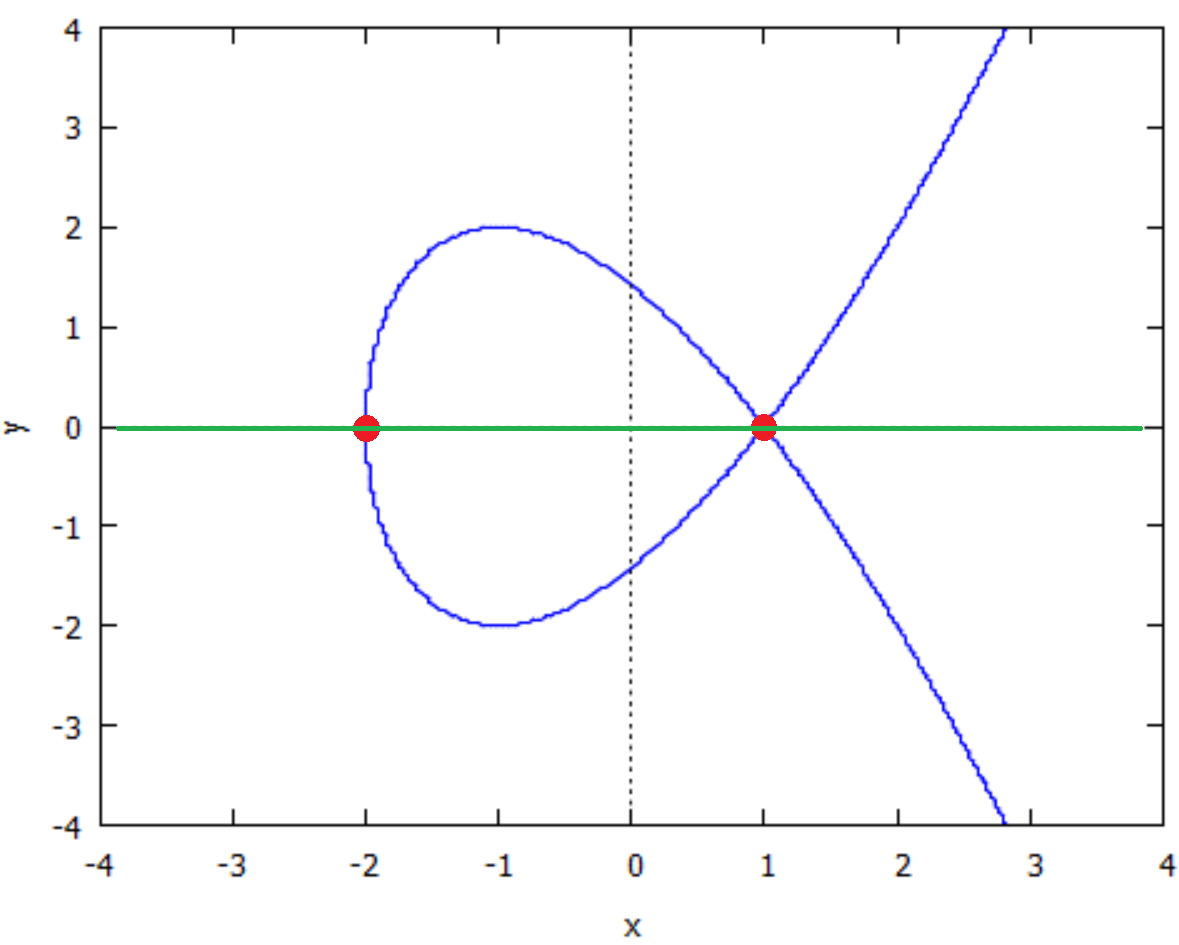
\includegraphics[width=.55\linewidth]{singular_curve.png}
  \caption{Plot of $y^2 = x^3-3x+2 = (x-1)(x-1)(x+2)$, we have multiple roots at $x=1$, the green line represents an addition of the roots (the two red dots) and it is obvious that this green line does not intersect any other point in the curve and hence the addition operation is not closed.}
\label{fig:singular-curve}
\end{figure}
%

{\bf Problem 6.2} One rational solution to the equation $y^2 = x^3 − 2$ is $(3, 5)$. Find a rational solution with $x \neq 3$ by drawing the tangent line to $(3, 5)$ and computing the second point of intersection.

I don't really know how to draw so, we can use the same trick as the Proof on Page 127
%
\nbea
(y_1 + (x - x_1)\lambda)^2 & = & x^3 + ax + b
\neea
%
here $y_1 = 5,~x_1 = 3,~ a = 0,~ b = -2$ and $\lambda = (3x^2 + a) / (2y) = 27/10$ so
%
\nbea
(5 + (x - 3)\lambda)^2 & = & x^3 - 2 \\
25 + \lambda^2(x^2 - 6x + 9) & = & x^3 - 2
\neea
%
so the coefficient of $x^2$ is $\lambda^2$ while
%
\nbea
(x - 3)(x - 3)(x - x') & = & x^3 - x^2(x'+6) + x(6x' + 9) - 9x'
\neea
%
so the coefficient of $x^2$ is $(x' + 6)$ thus $x' + 6 = \lambda^2 \to x' = \lambda^2 - 6 = 129/100$, to get the $y$ we feed it back to the line equation
%
\nbea
(y - 5) & = & \lambda(x - 3) \\
y & = & \lambda\frac{129}{100} - 3\lambda + 5 \\
& = & \frac{383}{1000}
\neea
%
just to check if it's correct
%
\nbea
\left ( \frac{383}{1000} \right )^2 & = & \left ( \frac{129}{100}\right )^3 - 2 \\
\frac{146689}{1000000} & = & \frac{146689}{1000000}
\neea
%
which is point at $(1.29, 0.383)$, very close to zero, see Fig.~\ref{fig:Problem-6.2}
%
\begin{figure}
\centering
  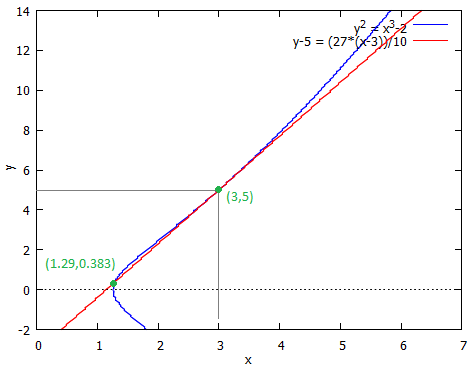
\includegraphics[width=.65\linewidth]{Problem_6_2.png}
  \caption{Plot of $y^2 = x^3-2$ (blue) and $y - 5 = \frac{27}{10}(x-3)$ (red), the first point of interest is $(3,5)$ and its tangent crosses the elliptic curve at $(1.29, 0.383)$.}
\label{fig:Problem-6.2}
\end{figure}
%

{\bf Problem 6.3}. Let $E$ be the elliptic curve over the finite field $K = \mathbb{Z}/5\mathbb{Z}$ defined by the equation
%
\nbea
y^2 = x^3 + x + 1.
\neea
%

(a) List all 9 elements of $E(K)$.

(b) What is the structure of $E(K)$, as a product of cyclic groups?

(a) Since it's just $K = \mathbb{Z}/5\mathbb{Z}$ we only have 5 different values of $x$, see Table~\ref{Tab:8}
%
\begin{table}[]
\centering
\caption{Various values of $x$ and $y$ that satisfy $y^2 = x^3 + x + 1$ in $K = \mathbb{Z}/5\mathbb{Z}$}
\label{Tab:8}
\begin{tabular}{|c|c|}
\hline
~~~$x$~~~ & ~~~$y$~~~ \\ \hline
0 & 1, 4 \\ \hline
2 & 1, 4 \\ \hline
3 & 1, 4 \\ \hline
4 & 2, 3 \\ \hline
\end{tabular}
\end{table}
%
Therefore there are 8 elements shown in Table~\ref{Tab:8}, $(0,1),(0,4),(2,1),(2,4),(3,1),(3,4),(4,2),(4,3)$, plus the point at infinity, $\{\mathcal{O}\}$, a total of 9 elements.

(b) Cyclic groups are groups that can be generated by just one element of the groups, first we need to note that the operation in question is addition of two points on the curve.

Next, this is a product of cyclic groups is because $(x,y) \in K \times K$, \ie $x$ and $y$ individually is an element of a cyclic group.

So our job here is to find the equivalent of the primitive root, an element that will generate the whole group by multiple applications of additions.

To find this ``primitive root'' we need to see if it can cover the whole 9 elements in the group by adding itself multiple times. We see from Table~\ref{Tab:9} that every element is a cyclic generator except for $(2,1),(2,4)$ and $\mathcal{O}$
%
\begin{table}[]
\centering
\caption{The self additive table of $(x,y) \in E(K)$ where $\times n$ means that the element is added to itself $n$ times and the order in the last column is the additive order}
\label{Tab:9}
\begin{tabular}{|c|c|c|c|c|c|c|c|c|c|}
\hline
~~~$\times1$~~~ & ~~~$\times2$~~~ & ~~~$\times3$~~~ & ~~~$\times4$~~~ & ~~~$\times5$~~~ & ~~~$\times6$~~~ & ~~~$\times7$~~~ & ~~~$\times8$~~~ & ~~~$\times9$~~~ & ~~~Order~~~ \\ \hline
(0,1) & (4,2) & (2,1) & (3,4) & (3,1) & (2,4) & (4,3) & (0,4) & $\mathcal{O}$ & 9 \\ \hline
(0,4) & (4,3) & (2,4) & (3,1) & (3,4) & (2,1) & (4,2) & (0,1) & $\mathcal{O}$ & 9 \\ \hline
(2,1) & (2,4) & $\mathcal{O}$ & (2,1) & (2,4) & $\mathcal{O}$ & (2,1) & (2,4) & $\mathcal{O}$ & 3 \\ \hline
(2,4) & (2,1) & $\mathcal{O}$ & (2,4) & (2,1) & $\mathcal{O}$ & (2,4) & (2,1) & $\mathcal{O}$ & 3 \\ \hline
(3,1) & (0,1) & (2,4) & (4,2) & (4,3) & (2,1) & (0,4) & (3,4) & $\mathcal{O}$ & 9 \\ \hline
(3,4) & (0,4) & (2,1) & (4,3) & (4,2) & (2,4) & (0,1) & (3,1) & $\mathcal{O}$ & 9 \\ \hline
(4,2) & (3,4) & (2,4) & (0,4) & (0,1) & (2,1) & (3,1) & (4,3) & $\mathcal{O}$ & 9 \\ \hline
(4,3) & (3,1) & (2,1) & (0,1) & (0,4) & (2,4) & (3,4) & (4,2) & $\mathcal{O}$ & 9 \\ \hline
\end{tabular}
\end{table}
%

{\bf Problem 6.4}. Let $E$ be the elliptic curve defined by the equation $y^2 = x^3 + 1$. For each prime $p \ge 5$, let $N_p$ be the cardinality of the group $E(\mathbb{Z}/p\mathbb{Z})$ of points on this curve having coordinates in $\mathbb{Z}/p\mathbb{Z}$. For example, we have that $N_5 = 6, N_7 = 12, N_{11} = 12, N_{13} = 12, N_{17} = 18, N_{19} =12, \dots , N_{23} = 24$, and $N_{29} = 30$ (you do not have to prove this).

(a) For the set of primes satisfying $p \equiv 2 \pmod{3}$, can you see a pattern for the values of $N_p$ ? Make a general conjecture for the value of $N_p$ when $p \equiv 2 \pmod{3}$.

(b) (*) Prove your conjecture.

(a) Cardinality is the order, \ie the number of elements of the group which in this case is denoted by $N_p$. From the list of $N_p$ given in the problem it looks like when $p \equiv 2 \pmod{3}$, $N_p = p+1$

(b) Note that the point at infinity, $\mathcal{O}$, is always a member so there are $p$ numerical members of the group. And to proceed we will definitely need the hint, I wouldn't expect automorphism or bijection to play a part here :)

First, the automorphism, the object of interest this time is the unity group $(\mathbb{Z}/p\mathbb{Z})^*$. Since this is a group the automorphism in question is just an isomorphism (a bijective morphism) from a group to itself, basically $x^3$ on $(\mathbb{Z}/p\mathbb{Z})^*$ is a bijection.

Now why is it the case that $x^3$ is a bijection? First we need to note that since $p$ is prime $(\mathbb{Z}/p\mathbb{Z})^*$ contains primitive roots, pick one of them say $g$. We can then list the members of $(\mathbb{Z}/p\mathbb{Z})^*$ as different powers of $g$
%
\nbea
g^1, g^2, g^3, \dots, g^{p-1}
\neea
%
where $g^{p-1} \equiv 1$.

{\bf Proposition 6.4.1}. Now $p \equiv 1 \pmod{3}$ (prime $p \equiv 0 \pmod{3}$ is an impossibility unless $p = 3$ but here $p \ge 5$) means that $p-1 \equiv 0 \pmod{3} = 3m$. The next important ingredient is to realize that two members of $(\mathbb{Z}/p\mathbb{Z})^*$, $g^a$ and $g^b$ are the same iff $a \equiv b \pmod{p-1}$.

For $p \equiv 1 \pmod{3} \to p-1 = 3m$, two cube of its members $g^{3a}$ and $g^{3b}$ are the same iff
%
\nbea
3a & \equiv & 3b \pmod{3m} \\
\bcancel{3}a & = & \bcancel{3}b + \bcancel{3}m\cdot k \\
a & \equiv & b \pmod{m}
\neea
%
So the cube, $g^{3a}$ and $g^{3b}$, of two members of $(\mathbb{Z}/p\mathbb{Z})^*$ with $p = 3m + 1$ are the same iff $a \equiv b \pmod{m}$. Now note that $a,b$ run from $1,\dots, 3m$.

This means that $x^3$ maps to only $m$ different values if $p = 3m+1$.

Back to our problem at hand, $p = 3m + 2$ and two cubes $g^{3a}$ and $g^{3b}$ can only be the same iff
%
\nbea
3a & \equiv & 3b \pmod{3m + 1} \\
3 (a - b) & = & (3m+1)k
\neea
%
Now $\gcd(3,3m+1) = 1$ therefore since $(3m+1)|3(a-b)$ it must be that $(3m+1)|(a-b)$ but this is not possible as $a,b$ run from $1, \dots, 3m+1$ so their (absolute) difference must be smaller than $3m+1$ therefore no two cube members $g^{3a}$ and $g^{3b}$ of $(\mathbb{Z}/p\mathbb{Z})^*$ with $p = 3m + 2$ can be the same.

This means that $x^3$ maps to $3m+1$ different numbers and thus $x^3$ is an automorphism on $(\mathbb{Z}/p\mathbb{Z})^*$ with $p = 3m + 1$. Since $x^3$ is a bijection on the unity group $(\mathbb{Z}/p\mathbb{Z})^*$, $x^3 + 1$ maps $1, 2, \dots, p-1$ to $2, 3, \dots, p-1, p \equiv 0$.

Therefore $x^3 + 1$ applied on $\mathbb{Z}/p\mathbb{Z}$ will map $0, 1, 2, \dots, p-1$ to $1, 2, 3, \dots, p-1, p \equiv 0$ and so every member of $\mathbb{Z}/p\mathbb{Z}$ is covered in a bijective way.

Furthermore, we know that every member, $w$, of the unity group $(\mathbb{Z}/p\mathbb{Z})^*$ that is an even power of a primitive root, $w \equiv g^{2n}$, is a quadratic residue, therefore there are $\frac{(p-1)}{2}$ quadratic residues.

Thus since $y^2 = x^3 + 1$ there are $\frac{(p-1)}{2}$ different values of $y^2$ and $2 \times \frac{(p-1)}{2} = p-1$ different values of $y$. Then there's also $y^2 = (-1)^3 + 1 = 0$, so that's one more value of $y$ and finally $\mathcal{O}$ itself so in total there are $N_p = (p - 1) + 1 + 1 = p + 1$ solutions.

{\bf Problem 6.7}. Suppose $y^2 = x^3 +ax+b$ with $a, b \in \mathbb{Q}$ defines an elliptic curve. Show that there is another equation $Y^2 = X^3 + AX + B$ with $A, B \in \mathbb{Z}$ whose solutions are in bijection with the solutions to $y^2 = x^3 +ax+b$.

First, let $a = r/s,~b = u/v$. The next question is whether $x,y$ themselves are rationals or real numbers, the same goes with $X,Y$ whether they are integers or real numbers, well we shall see, for starter let's assume $x,y \in \mathbb{Q},~~ x \to x/x', y \to y,y' $ then
%
\nbea
y^2 & = & x^3 +ax+b \\
\to \left (\frac{y}{y'} \right )^2 & = & \left ( \frac{x}{x'} \right )^3 +\frac{r}{s}\frac{x}{x'}+\frac{u}{v}
\neea
%
to change the $a,b$ coefficient to integers we need to multiply both sides by the common denominator and here the common denominator is $(y'^2x'^4sv)$. The goal then is to absorb it into $y$ and $x$. For $y$ we need something to an even power while for $x$ we need something to a power of multiple of three, the easiest choice would be to multiply both sides with $(y'^2x'^4sv)^{2\times3=6}$
%
\nbea
(y'^2x'^4sv)^6 \left (\frac{y}{y'} \right )^2 & = & (y'^2x'^4sv)^6 \left ( \frac{x}{x'} \right )^3 + (y'^2x'^4sv)^6 \frac{r}{s}\frac{x}{x'} + (y'^2x'^4sv)^6 \frac{u}{v} \\
(y'^5x'^2s^3v^3~y)^2 & = & (y'^4 x'^7 s^2 v^2~x)^3 + (y'^8x'^{16} s^3 v^4) \cdot (y'^4 x'^7 s^2 v^2~x) + (y'^{12}x'^{24} s^6 v^5 u) \\
\to Y'^2 & = & X'^3 + A'X' + B'
\neea
%
The above almost works except that  $A', B'$ are now no longer constant because they depend on $x', y'$ and this cannot be.

Therefore we cannot restrict $X,Y$ to be integers (and hence there shouldn't be any restriction on $x,y$ either although if $x,y$ are rationals so will be $X,Y$).

If we repeat the above process but this time only multiplying by $(sv)^{2\times3=6}$ we get
%
\nbea
(sv)^6 y^2 & = & (sv)^6 x^3 + (sv)^6 \frac{r}{s}x + (sv)^6 \frac{u}{v} \\
(s^3v^3~y)^2 & = & (s^2 v^2~x)^3 + (s^3 v^4) \cdot (s^2 v^2~x) + (s^6 v^5 u) \\
\to Y^2 & = & X^3 + AX + B
\neea
%
where $Y = s^3v^3~y, ~ X = s^2 v^2~x, ~ A = s^3 v^4$, and $B = s^6 v^5 u$ and this is clearly a bijection :)

{\bf Problem 6.8}. Suppose $a, b, c$ are relatively prime integers with $a^2 + b^2 = c^2$ . Then there exist integers $x$ and $y$ with $x > y$ such that $c = x^2 + y^2$ and
either $a = x^2 - y^2 , b = 2xy$ or $a = 2xy, b = x^2 - y^2$.

Since $a, b, c$ are relatively prime then $a$ and $b$ must not be both even. Can they be both odd? The answer is no because if we express them in modulo 4, a square can only be 0 or 1 modulo 4 and a sum of two odd squares would amount to 2 modulo 4, however, 2 is not a quadratic residue modulo 4.

Thus $a$ and $b$ must be of opposite parities (\ie one is odd and the other even), we then proceed by taking $b$ as odd (which doesn't affect the final result)
%
\nbea
a^2 + b^2 & = & c^2 \\
\to a^2 & = & c^2 - b^2 \\
& = & (c + b)(c - b)
\neea
%
since $c$ and $b$ are both odd we can express $2u = c+b, 2v = c-b \to c = u+v, b = u - v$ therefore $\gcd(u,v)=1$ because otherwise $c$ and $b$ would not be coprime.

Since $u$ and $v$ are coprime they must be perfect squares because $a^2 = 4uv$, \ie $u = x^2, v = y^2$ and
%
\nbea
a^2 & = & 4x^2y^2 \\
a & = & 2xy
\neea
%
substituting this into
%
\nbea
c & = & u + v \\
& = & x^2 + y^2 \\
b & = & u - v \\
& = & x^2 - y^2
\neea
%
and we are done (we can always $a \leftrightarrow b$ to get the other result). One small note is that $\gcd(x,y)=1$ because otherwise $a,b,c$ would not be coprime.

{\bf Problem 6.9} (*) Fermat’s Last Theorem for exponent $4$ asserts that any solution to the equation $x^4 + y^4 = z^4$ with $x, y, z \in \mathbb{Z}$ satisfies $xyz = 0$. Prove Fermat’s Last Theorem for exponent $4$, as follows.

(a) Show that if the equation $x^2 + y^4 = z^4$ has no integer solutions with $xyz \neq 0$, then Fermat’s Last Theorem for exponent 4 is true.

(b) Prove that $x^2 +y^4 = z^4$ has no integer solutions with $xyz \neq 0$ as follows. Suppose $n^2 +k^4 = m^4$ is a solution with $m > 0$ minimal among all solutions. Show that there exists a solution with $m$ smaller using Exercise 6.8 (consider two cases).

Part (a) is quite simple, suppose $x^2 + y^4 = z^4$ has no non trivial integer solution, and we now assume FLT 4 has a non trivial solution say $a^4 + b^4 = c^4$ then
%
\nbea
a^4 + b^4 & = & c^4 \\
(a^2)^2 + b^4 & = & c^4 \\
a'^2 + b^4 & = & c^4
\neea
%
with $a' = a^2$, hence $x^2 + y^4 = z^4$ has a non trivial integer solution which is a contradiction

Part (b) is quite difficult :) A simpler problem would be to prove $x^4 + y^4 = z^2$ has no non trivial integer solution but that's another problem. We can tackle this problem using Problem 6.8 this way, if $x^2 + y^4 = z^4 \to x^2 + (y^2)^2 = (z^2)^2$ has a solution then there are two possibilities
%
\nbea
\begin{array}{r c l c r c l}
x & = & 2ab & ~~~~~~~ & x & = & a^2 - b^2\\
y^2 & = & a^2 - b^2 & ~~~~~~~ & y^2 & = & 2ab
\end{array}
\neea
%
while $z$ is always $z^2 = a^2 + b^2$, the hint is actually to generate a smaller solution once you have one, \ie the infinite descent method first proposed by Fermat himself.

But I'm not going to do it that way :) I'll do it this way instead. First I factorize
%
\nbea
x^2 = z^4 - y^4 & = & (z^2 - y^2)(z^2 + y^2)
\neea
%
We know that $x,y^2,z^2$ form a Pythagorean triplet. Since $x^2$ is positive we know that $z > y$ and therefore $z$ must be odd, $y$, however, can be either even or odd ($z$ must be odd because according to the Pythagorean triplet formula $z^2 = m^2 + n^2$ with $m$ and $n$ having opposite parities).

Because they are Pythagorean triplet, we only need to consider pairwise coprime solutions, \ie $\gcd(z^2,y^2)=\gcd(z^2,x)=\gcd(y^2,x)=1$. But this means that $x$, $y$, $z$ must be coprime as well.

First if there's a common divisor $d$ between $(z^2 - y^2)$ and $(z^2 + y^2)$ then
%
\nbea
d &|& 2z^2 \\
d &|& 2y^2
\neea
%
Thus $d=1,2$ since $z$ and $y$ are coprime, therefore the only common divisors between $(z^2 - y^2),(z^2 + y^2)$ are either 1 or 2 which is expected since if $z$ and $y$ have opposite parities then the common divisors between them must be 1 and if $z$ and $y$ are both odd then the common divisor between $(z^2 - y^2)$ and $(z^2 + y^2)$ is 2.

If the common divisor of $(z^2 - y^2)$ and $(z^2 + y^2)$ is 1 then by virtue of $x^2 = (z^2 - y^2)(z^2 + y^2)$ we have
%
\nbea
z^2 - y^2 & = & a^2 \\
z^2 + y^2 & = & b^2
\neea
%
with $\gcd(a,b) = 1$ which means that $a$ and $b$ are odd. If the common divisor $(z^2 - y^2),(z^2 + y^2)$ is 2 then we have
%
\nbea
\begin{array} {r c l}
z^2 - y^2 & = & 2c^2 \\
z^2 + y^2 & = & 2d^2
\end{array}
\neea
%
with $\gcd(c,d) = 1$. We can rearrange the above ``judiciously'' to get
%
\nbea
y^2 & = & d^2 - c^2 \\
z^2 & = & d^2 + c^2
\neea
%
Note that $c,d,z,y$ are all pairwise coprime, also since $z$ and $y$ are both odd, according to the Pythagorean triplet formula $c$ has to be even and $d$ has to be odd (to see this, from the first equation $y^2 = d^2 - c^2 \to y^2  + c^2= d^2$ and the largest number, $d$, is always odd).

In either case we actually generate two other Pythagorean triplets $z^2 = y^2 + a^2$ and $z^2 + y^2 = b^2$ with four coprime variables (in the second case $d$ plays the role of $z$ of the first case, and $c \leftrightarrow y$, $y \leftrightarrow a$, $z \leftrightarrow b$). So now we can just concentrate on the first case where $z$ is odd, $y$ is even, $a$ is odd, and $b$ is odd.

From $z^2 = y^2 + a^2$ we have 
%
\nbea
z & = & m^2 + n^2 \\
y & = & 2mn \\
a & = & m^2 - n^2
\neea
%
while from $z^2 + y^2 = b^2$ we get
%
\nbea
z & = & e^2 - f^2 \\
y & = & 2ef \\
b & = & e^2 + f^2
\neea
%
Therefore
%
\nbea
y = \bcancel{2}mn & = & \bcancel{2}ef
\neea
%
From $ef = mn$ we have
%
\nbea
m & = & dm' \\
f & = & df' \\
n & = & f' n' \\
e & = & m'n'
\neea
%
which means that $\gcd(m,f) = d$ and $\gcd(e,n) = n'$, of course $d$ or $n'$ can be 1 but they cannot both be 1 at the same time because if they are then $e = m, f = n$ and 
%
\nbea
z = e^2 - f^2 & = & m^2 + n^2 \\
m^2 - n^2 & = & m^2 + n^2 \\
0 & = & 2n^2 \\
\to n & = & 0
\neea
%
which also means that $y=0$ a trivial solution. Now for a nontrivial solution
%
\nbea
z = e^2 - f^2 & = & m^2 + n^2 \\
e^2 - n^2 & = & m^2 + f^2 \\
n'^2(m'^2 - f'^2) & = & (m^2 + f^2) \\
n'^2(m'^2 - f'^2)\times(m^2-f^2) & = & (m^2 + f^2)\times(m^2 - f^2) \\
n'^2(m'^2 - f'^2)(m'^2-f'^2) d^2 & = & (m^4 - f^4) \\
n'^2(m'^2 - f'^2)^2d^2 & = & (m^4 - f^4) \\
\xi^2 & = & m^4 - f^4
\neea
%
where $\xi = n'(m'^2-f'^2)d$, now since $z = m^2 - n^2$ and $y = 2ef$ it means that $m < z$ and $f < y$ which means that we have an infinite descent because we can repeat the whole argument from the top about $z^4-y^4=x^2$ by replacing $z,y,x \leftrightarrow m,f,\xi$.

In the above if $d = \gcd(m,f)>1$ is true, we can just divide all terms $m,f,\xi$ by $d$ and the argument about infinite descent will still stand.

{\bf Problem 6.10}. This problem requires a computer.

(a) Show that the set of numbers $59 + 1 \pm s$ for $s \le 15$ contains 14 numbers that are $B$-power smooth for $B = 20$.

(b) Find the proportion of primes $p$ in the interval from $10^{12}$ and $10^{12} + 1000$ such that $p - 1$ is $B = 10^5$ power smooth.

(a) I don't really quite get the point of $59 + 1$, isn't it just $60$? \dunno Well, the set of numbers here is 45 to 75. Writing the code to do this is quite straightforward, and it was the first time I did coding on Maxima, here's the code
%
\begin{verbatim}
t:0;
for j:(59+1-15) thru (59+1+15) do
block(
    a:ifactors(j),
    b:0,
    block(
        for k:1 thru length(a) do
        block(
            if (a[k][1]^a[k][2] > 20) then b:1
        )
    ),
    if (b = 0) then 
    block(
        display(j),
        t:t+1
    )  
);
display(t);
\end{verbatim}
%
In the above code the variable $t$ is the total number of $B$-smooth numbers and $b$ is a just a flag that is set when a number is not $B$-smooth. I have used the function $ifactors$ to factorize a number, the result of this function call is as follows, \eg $ifactors(43) = \lbrack\lbrack2,1\rbrack,\lbrack23,1\rbrack\rbrack$ which means $43 = 2^1 \cdot 23^1$

(b) There are 140 out of 1001 numbers that are $B$-smooth, the code (using the same convention as part (a)) is as follows
\begin{verbatim}
t:0;
for i:1000000000000 thru (1000000000000+1000) do
block(
    a:ifactors(i),
    b:0,
    for j:1 thru length(a) do
    block(
        if (a[j][1]^a[j][2] > 100000) then b:1
    ),
    if (b = 0) then 
    block (
        display(i),
        t:t+1
    )
);
display(t);
\end{verbatim}


















\end{document}